\documentclass[fleqn, final]{../styles/unmphythesis}
\usepackage{../styles/qxd}
\renewcommand{\thechapter}{2}
%\newcommand{\thechapter}{1}

\makeindex
\begin{document}

%<*quantumdynamics>

\chapter{Quantum dynamics of atom-light interaction}
\section{Introduction}
In the last chapter, we have treated the light as continuous field that is a classical object. 
In this chapter, we will fully quantize the optical field and study the quantum noise origin of the light, the quantum dynamics of the atom-light interaction, and finally introduce the quantum non-demonlition measurement and spin squeezing. 

\section[Stokes vector description of photons' polarization measurement]{Stokes vector space description of the polarization of a quantized optical field}


\section{Dispersive atom-light interaction in the Heisenberg-Langevin picture}
The Lippmann-Schwinger solution, \erf{Eq::ScatteredField}, determines the input-output relation for linear atomic response given by the polarizability tensor $\tensor{\alpha}$.  In this section we derive the fully quantum mechanical description of dispersive atomic response and input-output relations for the quantized guided modes.  Following closely Ref. \cite{LeKien2005a}, we use a Heisenberg-Langevin approach for one-dimensional systems.  

The positive frequency component of the quantized electric field operator decomposes into guided and radiation (unguided) modes, $\hat{\mathbf{E}}^{(+)}=\hat{\mathbf{E}}_g^{(+)}+\hat{\mathbf{E}}_{r}^{(+)}$, where
	\begin{align}
		\hat{\mathbf{E}}_g^{(+)}(\br) &= \sum_{f,p} \int \mathrm{d}\omega  \sqrt{\frac{ \hbar \omega}{ v_g}} \awg \mathbf{u}_\mu (\br\!_\perp) e^{i f\beta(\omega) z } ,\label{Eq::QuantizedElectricField} \\
		\hat{\mathbf{E}}_r^{(+)}(\br) &= \sum_{m,p} \int \mathrm{d}\omega   \int_{-kn_2}^{kn_2}\mathrm{d}\beta \, \sqrt{ \hbar \omega}\awr \mathbf{u}_\nu (\br\!_\perp) e^{i\beta(\omega) z },
	\end{align}
The four HE$_{11}$ guided modes are indexed by $\mu =(\omega, f, p)$ for two polarizations $p$ and two propagation directions $f=\pm1$ with wavenumbers $f\beta (\omega)$.  The radiation modes are indexed by  $\nu=(\omega, \beta, m, p)$ where $\omega$ is the frequency, $m$ is the azimuthal quantum number (angular momentum), $p$ labels the two orthogonal polarizations. The longitudinal propagation constant $\beta(\omega)$ can vary from $-kn_2$ to $kn_2$, with $k = \omega/c$ \cite{Sondergaard2001,LeKien2005a}.  The creation/annihilation operators satisfy the usual continuous-mode commutation relations, $[\hat{a}_\mu, \hat{a}^\dag_{\mu'} ] = \delta_{f,f'} \delta_{p,p'} \delta ( \omega - \omega ') $, $[\hat{a}_\nu ,\hat{a}^\dag_{\nu'} ] = \delta_{m,m'} \delta_{p,p'} \delta ( \omega - \omega ')  \delta ( \beta - \beta') $.

The Hamiltonian for the system is
\begin{equation}
\hat{H} = \hat{H}_F+\hat{H}_A + \hat{H}_{\inter}.
\end{equation}
The free field Hamiltonian decomposes into guided and unguided modes, 
	\begin{equation}
		\hat{H}_F = \sum_{f,p}\int \mathrm{d}\omega \, \hbar \omega \hat{a}^\dagger_\mu \hat{a}_\mu 
+\sum_{m,p} \int \mathrm{d}\omega  \int_{-k n_2}^{k n_2} \mathrm{d}\beta \, \hbar \omega 
\hat{a}^\dagger_\nu \hat{a}_\nu.
	\end{equation}
We consider here alkali atoms with hyperfine multiplets of ground and excited levels, $\{ 
\ket{g}=\ket{nS_{1/2}, F, M_F}\}$, $\{ \ket{e} =\ket{nP_{J'}, F', M_{F'}}\}$,
	\begin{equation}
		\hat{H}_A  = \sum_g E_g \hat{\sigma}_{gg} + \sum_e E_e \hat{\sigma}_{ee},
	\end{equation}
with atomic transition operators $\hat{\sigma}_{ij} \equiv \ket{i}\bra{j}$.  In the rotating wave approximation, the atom-field interaction Hamiltonian is
	\begin{align}
		\hat{H}_{\inter} &= -\hat{\mathbf{d}}\cdot \hat{\mathbf{E}} =-\sum_{e,g} \left[ \hat{\mathbf{d}}_{eg}\cdot 
\hat{\mathbf{E}}^{(+)}(\br')+\hat{\mathbf{d}}_{ge}\cdot \hat{\mathbf{E}}^{(-)}(\br') \right],
	\end{align}
where the atomic dipole operator is projected between excited and ground subspaces, $\hat{\mathbf{d}}_{eg}= \hat{P}_e \hat{\mathbf{d}} \hat{P}_g $. The interaction Hamiltonian then takes the form, 
\begin{equation}
	\hat{H}_{\inter} = -\sum_{e,g} \left(\sum_{f,p} \int\mathrm{d}\omega \; \hbar g_{\mu, e,g}\, \hat{a}_\mu  \, 
		\hat{\sigma}_{eg}+ \sum_{m,p} \int\mathrm{d}\omega \! \int_{-kn_2}^{kn_2}\mathrm{d}\beta \,  \hbar 
g_{\nu, e,g}\, \hat{a}_\nu \, \hat{\sigma}_{eg}\right) + {H.c.},
	\end{equation}
where the coupling constants between the electric dipole and the guided/radiation modes are
\begin{subequations} \label{Eq::CouplingConstants}
	\begin{align}
		\hbar g_{\mu, e,g} &= \sqrt{\frac{\hbar \omega}{ v_g  }}\, \bra{e} \hat{\mathbf{d}} \ket{g} 
\cdot\mathbf{u}_\mu ( \br'\!_\perp ) e^{i f \beta(\omega)z} , \\
		\hbar g_{\nu, e,g} &= \sqrt{  \hbar \omega } \, \bra{e} \hat{\mathbf{d}} \ket{g} \cdot \mathbf{u}_\nu ( \br'\!_\perp ) e^{i\beta(\omega)z}  .
	\end{align}
\end{subequations}
The Heisenberg equations of motion thus follow,
	\begin{align}
		\der{\hat{a}_\mu} &= -i\omega \hat{a}_\mu +i\sum_{e,g} g_{\mu, e,g}^* \hat{\sigma}_{ge} \label{eq:da}\\
		\der{\hat{a}_\nu} &= -i\omega \hat{a}_\nu +i\sum_{e,g} g_{\nu, e,g}^*  \hat{\sigma}_{ge}\label{eq:danu}\\
		\der{\hat{\sigma}_{ge}} &= -i\omega_{eg} \hat{\sigma}_{ge} \label{Eq::dsigma}  \\
			&+ i\!\int_0^{\infty}\!\!\!\!\! \mathrm{d}\omega \sum_{e',g'} \bigg[ \big(\delta_{ee'} \hat{\sigma}_{gg'} \!-\! \delta_{gg'} \hat{\sigma}_{e'e} \big) \bigg\{ \sum_{f,p}  g_{\mu, e',g'}\hat{a}_\mu (\omega; t) \!+\! \sum_{m,p} \!\int_{-kn_2}^{kn_2}\!\!\!\!\!\! \mathrm{d}\beta \; g_{\nu, e',g'} \hat{a}_\nu(\omega, \beta; t) \bigg\} \bigg]. \nonumber
	\end{align}
Integrating the field equations, 
\begin{subequations}\label{eq:aout1}
\begin{align}
\hat{a}_\mu(\omega; t) &= \hat{a}_\mu(\omega; t_0) e^{-i\omega (t-t_0)} +i \sum_{e,g} g_{\mu,e,g}^* \int_{t_0}^t 
\mathrm{d} t' e^{-i\omega (t-t')}\hat{\sigma}_{ge}(t') \label{Eq::aguidedEOM}
\end{align}
\begin{align}
\hat{a}_\nu (\omega; t) &= \hat{a}_\nu (\omega; t_0) e^{-i\omega (t-t_0)} +i \sum_{e,g} g_{\nu,e,g}^* \int_{t_0}^t \mathrm{d} 
t' e^{-i\omega (t-t')}\hat{\sigma}_{ge}(t'),
\end{align}
\end{subequations}
substituting into \erf{Eq::dsigma}, and making the usual Markov approximation, $\int_0^\infty \mathrm{d}\omega e^{-i\omega (t-t')} |g(\omega)|^2\hat{\sigma}_{ge}(t')\approx \pi \delta(t-t')|g(\omega_{eg})|^2\hat{\sigma}_{ge}(t)$~\cite{?}, gives an expression for the ground-excited state coherences,
\begin{align}
&\dt{\hat{\sigma}_{ge}} =-i\omega_{eg} 
\hat{\sigma}_{ge}-\sum_{e'}\frac{\Gamma_{ee'}}{2}\hat{\sigma}_{ge'}  \label{eq:dsigmagedt1}\\
&+i \sum_{e',g'}\bigg[ (\delta_{e,e'} \hat{\sigma}_{gg'} - \delta_{g,g'} 
\hat{\sigma}_{e'e})\int_0^{\infty}\!\!\!\!\!\mathrm{d}\omega \bigg\{\sum_{f,p}  g_{\mu, e',g'} \hat{a}_\mu (t_0) 
+\sum_{m,p}  \int_{-kn_2}^{kn_2}\!\!\!\!\!\mathrm{d}\beta  g_{\nu, e',g'} \hat{a}_\nu(t_0) \bigg\} e^{-i\omega 
(t-t_0)}\bigg], \nonumber
\end{align}
where the decay of excited-state correlations is given by 
	\begin{equation}
		\Gamma_{ee'} = 2\pi \sum_{\mu,g} g_{\mu,e,g}g^*_{\mu,e',g} \vert_{\omega=\omega_{eg}}+2\pi 
\sum_{m,p,g} \int d\beta \, g_{\nu,e,g}g^*_{\nu,e',g} \vert_{\omega=\omega_{eg}}, \label{Eq::TotaleeDecayRate}
	\end{equation}
and the small energy shift is absorbed into the transition frequency $\omega_{eg} = (E_e - E_g)/\hbar$.  Equation (\ref{Eq::TotaleeDecayRate}) captures the modification of the spontaneous emission rate due to the nanofiber, which alters the local density of states \cite{LeKien2005a}.  The first sum describes decay into the guided modes and the second into the unguided radiation modes \cite{ Nha1997,Klimov2004,LeKien2005a,Maslov2006}. The decay rate of a given excited state into all the guided modes is given by
	\begin{equation}
		\Gamma_e^{\oneD}= 2\pi \sum_{\mu,g} |g_{\mu,e,g} |^2_{\omega = \omega_{eg}} =  \frac{ 2\pi }{\hbar} \frac{ \comment{\omega_{eg}} }{v_g} \sum_{\mu,g} \big|\bra{e}\hat{\mathbf{d}}\ket{g} \cdot \mathbf{u}_{fp}(\br'_\perp)\big|^2  .
	\end{equation}
This agrees with the expected expression following from the guided-mode contribution to the dyadic Green's function, \erf{Eq::ImGreenLocal},
	\begin{equation}
		\Gamma_e^{\oneD} =  \frac{2}{\hbar} \sum_{g}  \bra{g}\hat{\mathbf{d}}\ket{e}\cdot 
\Im \Big[\tensor{\mathbf{G}}^{(+)}_g(\br', \br'; \omega_{eg} ) \big] \cdot \bra{e}\hat{\mathbf{d}}\ket{g} ,
	\end{equation}
enhanced over the free-space rate by the Purcell factor.  In general, the decay rate into a given mode depends on the dipole orientation \cite{Klimov2004, Vos2009}. Recently, it was predicted \cite{LeKien2014a} and demonstrated \cite{Mitsch2014a} that the decay rates into the forward and backward modes are not always equal.  Specifically, when the atomic dipole has a component rotating in the plane defined by the atom and nanofiber, the relative decay rates can differ due to the longitudinal component of the guided modes. \comment{Maybe we should include a plot of $\Gamma_{\rm 1D}/\Gamma_0$.  This is the \emph{first} thing people ask.  We must make the point that while it's not so large, we can benefit from many atoms much more easily than other systems, such as those alligator waveguide photonic crystals.}

Here we are interested in linear response for excitation far from resonance.  We follow Ref. \cite{LeKien2014a} and consider an atom sufficiently far from the fiber surface such that the modification of the spontaneous emission rate is small.   In this case the decay rate is approximated as $\Gamma_{ee'} \approx \delta_{e,e'} \Gamma_{e}$ (\comment{it is confusing here -- more details or references?}), where $\Gamma_e$ is the total decay rate from excited state $\ket{e}$, given by the diagonal elements of \erf{Eq::TotaleeDecayRate}.  \comment{In steady state}, by defining $ \hat{\sigma}_{ge'}(t)=\int \frac{\mathrm{d}\omega}{\sqrt{2\pi}}\hat{\sigma}_{ge'}(\omega) e^{-i\omega(t-t_0)} $, the dipole operator (from Equ.~\eqref{eq:dsigmagedt1}) in the linear regime ($\hat{\sigma}_{ee'} \rightarrow 0 $) is approximately
	\begin{align}\label{eq:sigmagetint}
		\hat{\sigma}_{ge}(t) \approx -\int_0^{\infty}\mathrm{d}\omega \sum_{g'} \hat{\sigma}_{gg'}\bigg( & \sum_{f,p}  
\frac{g_{\mu, e,g'}}{\omega-\omega_{eg} \error{+} i \Gamma_{e}/2  }\, \hat{a}_\mu (t_0) \\
	+& \sum_{m,p} \int_{-kn_2}^{kn_2}\mathrm{d}\beta \, \frac{g_{\nu, e,g'}}{\omega-\omega_{eg} \error{+} i \Gamma_{e}/2 } \,\hat{a}_\nu (t_0)  \bigg)e^{-i\omega (t-t_0)} . \nn
	\end{align}
By definition, in the frequency domain, 
\begin{align}\label{eq:sigmageomega}
		\hat{\sigma}_{ge}(\omega) \approx - \sqrt{2\pi}\sum_{g'} \hat{\sigma}_{gg'}\bigg( & \sum_{f,p}  
\frac{g_{\mu, e,g'}}{\omega-\omega_{eg} \error{+} i \Gamma_{e}/2  }\, \hat{a}_\mu (t_0) \\
	+& \sum_{m,p} \int_{-kn_2}^{kn_2}\mathrm{d}\beta \, \frac{g_{\nu, e,g'}}{\omega-\omega_{eg} \error{+} i \Gamma_{e}/2 } \,\hat{a}_\nu (t_0)  \bigg) . \nn
\end{align}
Using the definition of $ \sigma_{ge}(\omega) $ in the frequency domain ($ t\gg t_0 $), Equ.~\eqref{Eq::aguidedEOM} implies the input-output relationship that
\begin{align}\label{Eq::aguidedomega}
\hat{a}_\mu(\omega;t )e^{i\omega t} &= \hat{a}_\mu(\omega;t_0)e^{i\omega t_0} +i \sqrt{2\pi}\sum_{g,e}g_{\mu,e,g}^*(\omega)\hat{\sigma}_{ge}(\omega). 
\end{align}
By substituting Equ.~\eqref{eq:sigmageomega} into \erf{Eq::aguidedomega} and defining asymptotic modes,  $\hat{a}^{\inp}(\omega) = \lim_{t_0\rightarrow -\infty} \hat{a}(t_0) e^{i\omega t_0}$, $\hat{a}^{\out}(\omega) = \lim_{t\rightarrow +\infty} \hat{a}(t) e^{i\omega t}$ \cite{Fan2010}, we obtain the input-output relationship for the guided modes,
\begin{align} \label{Eq::aout}
\hat{a}^{\out}_\mu (\omega) = \hat{a}^{\inp}_\mu (\omega) &- 2\pi i\sum_{p',f'} 
\sum_{e,g,g'}\!\hat{\sigma}_{gg'}\frac{ g_{\mu,e,g}^* g_{\mu',e,g'}}{ \Delta_{eg} \error{+} i \Gamma_{e}/2 }\hat{a}^{\inp}_{\mu'}(\omega) \\
&- 2\pi i\sum_{m,p} \sum_{e,g,g'} \int^{kn_2}_{-kn_2} d\beta \,\hat{\sigma}_{gg'}\frac{ g_{\mu,e,g}^* g_{\nu',e,g'}}{ \Delta_{eg} \error{+} i \Gamma_{e}/2 }\hat{a}^{\inp}_{\nu}(\omega),\nn
\end{align}
where $\Delta_{eg} = \omega - \omega_{eg}$.  The real part this relationship describes the coherent elastic scattering of photons from all modes--guided and radiation--into guided mode $\mu$, mediated by the atomic state.  The imaginary part describes loss from incoherent spontaneous emission into other modes.  For low atomic saturation, elastic scattering dominates and the interaction is purely dispersive. 

Equation (\ref{Eq::aout}) agrees with the expected form given by the Lippmann-Schwinger equation in the first Born approximation,
	\begin{equation} \label{Eq::IOScatteredField}
		\hat{\mathbf{E}}^{(+)}_{\out,g}(\br)=\hat{\mathbf{E}}^{(+)}_{ \inp, g}(\br)+\tensor{\mathbf{G}}_g^{(+)}(\br,\br',\comment{\omega_0})\cdot \poltens \cdot \Big[\hat{\mathbf{E}}^{(+)}_{\inp, g}(\br')+\hat{\mathbf{E}}^{(+)}_{\inp,r}(\br') \Big],
	\end{equation}
by noting
	\begin{equation}
		\int d^2 \mbf{r} \, \mathbf{u}^*_{\mu} (\br)\cdot \tensor{\mathbf{G}}_g^{(+)}(\br,\br',\comment{\omega_0})\cdot 
\poltens \cdot \mathbf{u}_{\mu'} (\br') =  i \frac{ 2\pi \omega_0}{v_g} \mathbf{u}^*_\mu 
 (\br') \cdot \poltens \cdot \mathbf{u}_{\mu'} (\br') = - i \frac{2 \pi}{\hbar} \sum_{e,g,g'}\!\ 
 \hat{\sigma}_{gg'} \frac{g_{\mu,e,g}^* g_{\mu',e,g'}}{ \Delta_{eg} \error{+} i \Gamma_{e}/2 }, 
	\end{equation}
where the guided-mode dyadic Green's function is given in \erf{Eq::GreensGuided} and the atomic polarizability operator is \cite{Buhmann2004, Deutsch2010a,LeKien2013a},
	\begin{equation} \label{Eq::PolarizabilityOperator}
		\poltens = - \frac{1}{\hbar} \sum_{e,g,g'}\ket{g}\frac{\bra{g}\hat{\mathbf{d}}\ket{e}\bra{e} 
\hat{\mathbf{d}}\ket{g'}}{\Delta_{eg}  \error{+} i \Gamma_{e}/2 }\bra{g'}.
	\end{equation}
	
Scattering of classical waves follows when the field is in a coherent state.  \comment{Explaining this well is of critical importance - while injection of a classical field does not change the Purcell effect or decay rate (which is tied to the atomic transition frequency) it does scatter into all field modes with the same frequency, thus promoting them from vacuum}.  The phase-shift on a guided mode with a given polarization $p$, \erf{Eq::PhaseShift}, now depends on the internal state of the atom.  Given an atom in a particular ground sublevel $\ket{g}$, this can be expressed \cite{LeKien2014a}
	\begin{equation} \label{Eq::PhaseShiftMultilevel}
		\delta  \phi_{p,g} =2\pi \frac{\comment{ \omega_{0}}}{v_g} \mathbf{u}^*_{+, p}(\br'_\perp) \cdot \Re \big[\bra{g} 
\hat{\tensor{\boldsymbol{\alpha}}} \ket{g} \big] \cdot \mathbf{u}_{+, p}(\br'_\perp) = -\frac{1}{\hbar} \sum_e \frac{ \comment{ \omega_{0} } }{v_g} \frac{2 \pi |\bra{e}\hat{\mathbf{d}}\ket{g} \cdot \mathbf{u}_{+,p}(\br'_\perp)|^2}{ \Delta_{eg} } ,
	\end{equation}
where $\Delta_{eg} = \omega_0 - \omega_{eg}$ is the laser detuning from the atomic transition frequency.  For large detuning, $\Gamma_{e}/\Delta_{eg} \ll 1$, the scattering is entirely elastic.  In this case, the absorption/scattering loss can be ignored and \erf{Eq::PhaseShiftMultilevel} describes a pure dispersive phase shift.







\section{Polarization spectroscopy and quantum nondemolition measurement for alkali atoms}
\subsection{Clock states as the pseudo-spin states for polarimetry}~\footnote{See the NanofiberInterface note and the AFOSRProposal (2010) for related discussions.}
Now, we use the $ f=3,\,m=0 $ and $ f=4,\,m=0 $ two sublevels of $ 6S_{1/2} $ ground state as the psuedo-spin to represent qubit. That is to say, $ \ket{\uparrow}=\ket{f=4,\,m=m_x=0} $ and $ \ket{\downarrow}=\ket{f=3,\,m=m_x=0} $, where we choose the $ x $-axis as the quantization axis. We also launch two orthogonal probe beams notated as mode $ H $ and mode $ V $, whose polarization axes are parallel or perpendicular to the $ x $-axis where the atom is lying in. We can quantize the propagating guided fields with duration $ \tau $ and photon number $ N_L $ as
\begin{align} \label{Eq::FiberModeFunctions}
		\hat{\mathbf{E}}^{(+)}(r\!_\perp,\phi,z) = \sqrt{ \frac{2 \pi \hbar \omega_0}{ v_g \tau} } \big( \mathbf{u}_H(r\!_\perp,\phi) \hat{a}_H + \mathbf{u}_V(r\!_\perp,\phi) \hat{a}_V \big) e^{i \beta z}.
\end{align}
\textcolor{red}{Note: We only consider the forward-propagating fields. Otherwise, it will mess up our results below.}

We are interested in developing a dispersive, state-dependent interface between the collective spin of these atoms and the guided field modes of the fiber.  We first consider the light-shift interaction for a single alkali atom interacting with detuned light in the guided modes of the tapered nanofiber.  Such an interaction is described by the effective Hamiltonian,
\begin{align}  \label{Eq::LightShiftHam}
	H_{\rm eff}   &= -\hat{\mathbf{E}}^{(-)}(r^\prime\!\!_\perp,\phi',z')\cdot \tensor{\alpha}\cdot \hat{\mathbf{E}}^{(+)}(r^\prime\!\!_\perp,\phi',z')\\
	&= -\frac{2\pi \hbar \omega_0}{ v_g\tau} \Big( \mathbf{u}^*_H(r^\prime\!\!_\perp, \phi')\! \cdot\! \tensor{\alpha}\! \cdot\! \mathbf{u}_{H}(r^\prime\!\!_\perp, \phi') \hat{a}\dg_H \hat{a}_H \nonumber\\
	&\quad\quad\quad\quad\quad +  \mathbf{u}^*_V(r^\prime\!\!_\perp, \phi') \!\cdot\! \tensor{\alpha}\! \cdot\! \mathbf{u}_{V}(r^\prime\!\!_\perp, \phi') \hat{a}\dg_V \hat{a}_V \\
	&\quad\quad\quad\quad\quad + \mathbf{u}^*_H(r^\prime\!\!_\perp, \phi') \!\cdot\! \tensor{\alpha}\! \cdot\! \mathbf{u}_{V}(r^\prime\!\!_\perp, \phi') \hat{a}\dg_H \hat{a}_V \nonumber\\
	&\quad\quad\quad\quad\quad + \mathbf{u}^*_V(r^\prime\!\!_\perp, \phi') \!\cdot\! \tensor{\alpha}\! \cdot\! \mathbf{u}_{H}(r^\prime\!\!_\perp, \phi') \hat{a}\dg_V \hat{a}_H \Big), \nonumber 
\end{align}
where the atom is positioned at $ (r^\prime\!\!_\perp,\phi',z') $. 
In the expansion above, the first two terms lead to the \emph{birefringent}\index{birefringence effect} coupling due to the different phase shifts between $ H $ and $ V $ modes. The second two terms lead to the \emph{Faraday}\index{Faraday effect!Faraday coupling} coupling due to a coherent redistribution of photons between $ H $ and $ V $ modes. The polarization dependence of the atom-probe coupling arises from two sources: the tensor nature of $ \tensor{\alpha} $ and the spatial dependence of $ \mathbf{u}_{H}(r\!_\perp, \phi) $ versus $ \mathbf{u}_{V}(r\!_\perp, \phi) $. The amplitude of the $ H $ mode is roughly $ 3 $ times larger than the $ V $ mode on the $ x $-axis. However, in the expression of the Hamiltonian there is always the atomic polarizability multiplied with the modes, which makes it a state-dependent problem. 

Note: alternatively, the effective Hamiltonian can also be rewritten using the irreducible tensor components as
\begin{align}  
H_{\rm eff} &= - \sum_{f,f'}\alpha_0(\Delta_{f,f'}) \left\{ C_{j'ff}^{(0)} \hat{\mathbf{E}}^{(-)} \cdot \hat{\mathbf{E}}^{(+)} \hat{\mathbbm{1}}_f \phantom{\frac{\hat{1}}{1}}\right. \nonumber\\
&\quad\quad\quad + i C_{j'ff'}^{(1)} \left(\hat{\mathbf{E}}^{(-)} \times \hat{\mathbf{E}}^{(+)} \right) \cdot \hat{ \mathbf{f}} \nonumber\\
&\quad\quad\quad  \left. + C_{j'ff}^{(2)} \hat{E}_i^{(-)} \hat{E}_j^{(+)} \left( \frac{ \hat{f}_i \hat{f}_j  + \hat{f}_j \hat{f}_i  }{2} - \frac{1}{3}\delta_{ij} \hat{ \mathbf{f}} \cdot \hat{\mathbf{f}}  \right) \right\}. \label{Eq::LightShiftHam_irep}
\end{align} 

In the weak excitation regime, we limit our attention to the clock state subspace, and hence the polarizability is restricted to the reduced tensor $ \bra{f,m=0}\tensor{\alpha}\ket{f,m=0}$, $f=3,4 $. We can denote such reduced atomic polarizability tensors as 
\begin{align}
\tensor{\alpha}_{\uparrow} &=\bra{f=4,m=0}\tensor{\alpha}\ket{f=4,m=0}\\
\tensor{\alpha}_{\downarrow} &=\bra{f=3,m=0}\tensor{\alpha}\ket{f=3,m=0}.
\end{align}


In the clock state subspace, the vector component of the atomic polarizability is always zeros due to the symmetry of quantum jumps. In the light-shift Hamiltonian expression (Equ.~\eqref{Eq::LightShiftHam}), the crossing terms involving products between both $ H $ and $ V $ modes vanish. 

Now that, the light shift Hamiltonian can be written as 
\begin{align}
H_{\rm eff} & = \frac{ \hbar }{ \tau}\Big( \chi_{H,\uparrow}\op{\uparrow}{\uparrow} +  \chi_{H,\downarrow} \op{\downarrow}{\downarrow} \Big) \hat{a}_H\dg \hat{a}_H \nonumber\\
&\quad +  \frac{ \hbar }{ \tau} \Big( \chi_{V,\uparrow}\op{\uparrow}{\uparrow} +  \chi_{V,\downarrow} \op{\downarrow}{\downarrow} \Big) \hat{a}_V\dg \hat{a}_V  \label{HeffLS}
\end{align}
where the single atom light shifts per photon or the coupling strengths for the different combination of clock states and polarizations are defined as
\begin{align}
\chi_{H,\uparrow} &=  -\frac{2\pi\omega_0}{v_g} \mathbf{u}^*_{H}(r^\prime\!\!_\perp,\phi') \cdot\tensor{\alpha}_{\uparrow}\cdot \mathbf{u}_{H}(r^\prime\!\!_\perp,\phi') \\
\chi_{H,\downarrow} &=  -\frac{2\pi\omega_0}{v_g} \mathbf{u}^*_{H}(r^\prime\!\!_\perp,\phi') \cdot\tensor{\alpha}_{\downarrow}\cdot \mathbf{u}_{H}(r^\prime\!\!_\perp,\phi') \\
\chi_{V,\uparrow} &=  -\frac{2\pi\omega_0}{v_g}  \mathbf{u}^*_{V}(r^\prime\!\!_\perp,\phi') \cdot\tensor{\alpha}_{\uparrow}\cdot \mathbf{u}_{V}(r^\prime\!\!_\perp,\phi')  \\
\chi_{V,\downarrow} &=  -\frac{2\pi\omega_0}{v_g}  \mathbf{u}^*_{V}(r^\prime\!\!_\perp,\phi') \cdot\tensor{\alpha}_{\downarrow}\cdot \mathbf{u}_{V}(r^\prime\!\!_\perp,\phi'). 
\end{align}

Suppose the probe laser is in a near resonance regime of the lower frequency side of the $ D_1 $ line so that the detuning from the ground $ 6S_{1/2} $ $ \ket{f=4} $ hyperfine level to the excited $ 6P_{1/2} $ $ \ket{f=3} $ hyperfine level is far greater than the hyperfine structure splitting of the excited states. We can then ignore the tensor component and the imaginary part of the atomic polarizability, as well as the higher level of excited states above the $ 6P_{1/2} $ energy levels. Baring that the vector component of the polarizability for the clock state vanishes, we only have the scalar coefficient $C_{j' f}^{(0)} =1/3  $ (from Equ.~\eqref{Eq::ScalarCoefSum}) non-zero.~\footnote{Similar case for the $ D_2 $ line will lead to $ C_{j' f}^{(0)} =2/3 $.} Therefore, the atomic polarizability can be given by
\begin{align}
\tensor{\alpha}_{\uparrow} &\approx\sum_{f'=3,4}\frac{\alpha_0(\Delta_{4,f'})}{3}\mathbbm{1} \\
\tensor{\alpha}_{\downarrow} &\approx\sum_{f'=3,4}\frac{\alpha_0(\Delta_{3,f'})}{3}\mathbbm{1},
\end{align}
with $ \alpha_0(\Delta_{f,f'})=-\frac{3\lambda_{j'j}^3}{32\pi^3} \frac{\Gamma}{\Delta_{f,f'}} $. In our case, we can make $ \lambda_{j'j}\approx\lambda= \frac{2\pi c}{\omega_0}$. Therefore, we have
\begin{align}
\frac{2\pi\omega_0}{v_g}\alpha_0(\Delta_{f,f'})=-\frac{n_g\sigma_0}{4} \frac{\Gamma}{\Delta_{f,f'}}
\end{align}
with the 3D atomic scattering cross section $ \sigma_0= \frac{3\lambda^2}{2\pi}  $. 

The coupling strength for the $ D_1 $ line probing can then be written as
\begin{align}
\chi_{H,\uparrow} &=   \frac{1}{2} \sum_{f'} \chi_{H0}(f',4) C_{j',f',4}^{(0)}  =  \frac{1}{2} \sum_{f'} \frac{\chi_{H0}(f',4)}{3} \label{chiHUp}  \\
\chi_{H,\downarrow} &=   \frac{1}{2} \sum_{f'} \chi_{H0}(f',3)  C_{j',f',3}^{(0)} = \frac{1}{2} \sum_{f'} \frac{\chi_{H0}(f',3) }{3} \label{chiHDown}\\
\chi_{V,\uparrow} &=   \frac{1}{2} \sum_{f'} \chi_{V0}(f',4)  C_{j',f',4}^{(0)}  =   \frac{1}{2} \sum_{f'} \frac{\chi_{V0}(f',4)}{3}\label{chiVUp}  \\
\chi_{V,\downarrow} &=   \frac{1}{2} \sum_{f'} \chi_{V0}(f',3)  C_{j',f',3}^{(0)}=   \frac{1}{2} \sum_{f'} \frac{\chi_{V0}(f',3) }{3} \label{chiVDown}
\end{align}
and 
\begin{align}
\chi_{H0}(f',f) &= \left( \frac{ \sigma_0}{A_{ef\!f}^H} \right) \left( \frac{\Gamma}{2 \Delta_{f,f'}} \right)\\
\chi_{V0}(f',f) &= \left( \frac{ \sigma_0}{A_{ef\!f}^V} \right) \left( \frac{\Gamma}{2 \Delta_{f,f'}} \right)\\
A_{ef\!f}^H &= \frac{1}{n_g|\mathbf{u}_{H}(r^\prime\!\!_\perp,\phi')|^2}\\
A_{ef\!f}^V &= \frac{1}{n_g | \mathbf{u}_{V}(r^\prime\!\!_\perp,\phi')|^2}.\label{eq:AeffV}
\end{align}
Considering the relationship between $ \Gamma_{1D} $ and $ \Gamma_{vac} $ (the same as the $ \Gamma $ above) from Equ.~\eqref{Gamma1DGammavac}, Equs.~\eqref{chiHUp} and~\eqref{chiHDown} are equivalent to Equ.~\eqref{phaseshiftGamma1D} derived from the Green's function method with scalar polarizability. The scalar polarizability factor of $ C_{j',f',f}^{(0)}=\frac{1}{3} $ in Equ.~\eqref{chiHUp} through Equ.~\eqref{chiVDown} indicates the possibility of transitions back to the clock state. This factor can be absorbed into the atomic scattering cross section by treating the scattering cross section as an average over all possible quantum transitions. 

\subsection{Full Hamiltonian using Clebsch-Gordan coefficients}
We can also work in the time-domain to include the wave-propagation process much carefully. \textcolor{red}{Note: part of the content below is directly from Ben's notes.}

For the nanofiber interface, we specify to the single-mode condition that only the HE$_{11}$ spatial mode propagates in the fiber with propagation constant $\beta_0$.  We can further make the first Markov approximation that the coupling is dominated by frequencies near an atomic transition frequency $\omega_0$ and then extend the limit of integration to $-\infty$ as a mathematical convenience.  We then define Fourier-transformed \emph{input-output field operators} that describe propagating modes in the nanofiber,
	\begin{align}
		\hat{a}_{\mu}(z,t) \equiv \frac{1}{\sqrt{2\pi}} \int_{-\infty}^{\infty} \mathrm{d}\omega \hat{a}_{\mu}(\omega) e^{i f \beta_0 z -i\omega_0 t}.
	\end{align}	
They satisfy the white-noise commutation relations
	\begin{align}
		[\hat{a}_{\mu}(z,t), \hat{a}\dg_{\mu'}(z',t')] = \delta_{p,p'} \delta_{f,f'} \delta(t-t' - |z-z'|/v_p).
	\end{align}	
Note that the commutation relation is related to the \emph{phase retarded time} which is related to the phase velocity, $v_p = \omega_0/\beta_0$, rather than the group velocity.  More details on this can be found in several of Le Kien's papers, including \emph{Correlations between photons emitted by multi-atom fluorescence into a nanofiber} (http://journals.aps.org/pra/pdf/10.1103/PhysRevA.77.033826).

The guided-mode electric field operator can then be written in terms of the input-output field operators
	\begin{align}
		\hat{\mathbf{E}}_g^{(+)}(\mathbf{r}) = \sum_{f ,p} \sqrt{\frac{2 \pi \hbar \omega_0}{v_g}} \hat{a}_{\mu}(z,t) \mathbf{u}_{\mu}(\mathbf{r}_\perp) 
	\end{align}
We have dropped the $\omega(\beta)$ label on the mode functions as it is only for the fundamental propagation constant $\beta_0$.

Atoms can be trapped around the surface of the nanofiber using a handful of techniques.  In the interaction Hamiltonian $z=z' =z_A$ for the two field operators that appear, so we drop the $z$ label on the field operators $\hat{a}(z,t) \rightarrow \hat{a}(t)$.  This will not in general be valid when calculating the output propagating field operators, as their interaction will depend on the positions of the multiple atoms throughout the ensemble.  However, we make the assumption that the transit time through the nanofiber region is short compared to the collective atomic dynamics, and thus we can ignore the retarded group time.  

From Equ.~\eqref{Eq::LightShiftHam}, the effective Hamiltonian of the light-atom interaction at time $ t $ can then be given by
\begin{align}  
	H_{\rm eff}   = -\frac{2\pi \hbar \omega_0}{ v_g } &\Big( \mathbf{u}^*_H(r^\prime\!_\perp, \phi') 
	\!\cdot\! 
	\tensor{\alpha} \!\cdot\! \mathbf{u}_{H}(r^\prime\!_\perp, \phi') \hat{a}\dg_H(t) \hat{a}_H(t) \nonumber\\
	&\!\! +  
	\mathbf{u}^*_V(r^\prime\!_\perp, \phi')\! \cdot\! 
	\tensor{\alpha} \!\cdot\! \mathbf{u}_{V}(r^\prime\!_\perp, \phi') \hat{a}\dg_V(t) \hat{a}_V(t) \nonumber\\
	&\!\! + \mathbf{u}^*_H(r^\prime\!_\perp, \phi')\! \cdot\! \tensor{\alpha}\! \cdot\! 
	\mathbf{u}_{V}(r^\prime\!_\perp, \phi') \hat{a}\dg_H(t) \hat{a}_V(t) \nonumber\\
	&\!\! + \mathbf{u}^*_V(r^\prime\!_\perp, \phi') \!\cdot\! \tensor{\alpha}\! \cdot\! 
	\mathbf{u}_{H}(r^\prime\!_\perp, 
	\phi') \hat{a}\dg_V(t) \hat{a}_H(t) 
	\Big).  \label{eq:LightShiftHam_CG}
\end{align}
The atomic polarizability tensor $\tensor{\alpha}$\index{polarizability!polarizability tensor} is composed of a dyad of vector dipole operators,    
\begin{align}
	\tensor{\alpha} & =  - \frac{1}{\hbar}  \sum_{F,F'} \frac{ \mathbf{d}_{FF'} \mathbf{d}^\dagger_{F'F} 
	}{\Delta_{FF'}+i\frac{\Gamma}{2} } \\
		& = \sum_{q,q'}  \sum_{F,F'} \sum_{m_1, m_2, m'} \!\!\!\!\!\! \alpha_0(F,F') \mathbf{e}_q \otimes 
		\mathbf{e}^*_{q'} | o^{J'F'}_{JF} |^2 C^{Fm_2;1q}_{F'm'} C^{Fm_1;1q'}_{F'm'} \op{F m_2}{F m_1},
\end{align}
with the vector raising  dipole operator,
\begin{align}
	\mathbf{d}^\dagger_{F'F} =  \bra{P_{J'}}| d |\ket{S_{1/2}} \sum_q \sum_{m,m'} \mathbf{e}_q^* 
	o^{J'F'}_{JF} C^{Fm;1q}_{F'm'} \op{F'm'}{Fm}
\end{align}
where $o^{J'F'}_{JF}$ is the oscillator strength from Ref. \cite{Deutsch2010a} and $C^{Fm;1q}_{F'm'} 
\equiv 
\ip{F'm'}{Fm;1q}$ is a Clebsch-Gordan coefficient. 
Notice that $m' = m_1 + q'$ and $m' = m_2 + q$ and thus
\begin{align}
	m_2 - m_1 = q-q'.
\end{align}
The characteristic polarizability\index{polarizability!characteristic polarizability} is
\begin{align} \label{eq:CharacteristicPolarizability}
	\alpha_0(F,F') = - \frac{ |\bra{P_{J'}}| d |\ket{S_{1/2}}|^2 }{\hbar (\Delta_{F,F'}+i\frac{\Gamma}{2})} = - 
	\frac{3 
	\lambda_{J'}^3}{32 \pi^3} \frac{\Gamma}{\Delta_{F,F'}+i\frac{\Gamma}{2}}.
\end{align}
and the detuning is defined as
\begin{align}
	\Delta_{FF'} \equiv \omega - (\omega_{F'} - \omega_{F}).
\end{align}
Due to the hyperfine ground splitting in Cs$^{133}$ of approximately 9.2 GHz, the characteristic 
polarizabilities for the two ground hyperfine manifolds, \erf{eq:CharacteristicPolarizability}, can in 
general have different magnitudes and signs.  Implied in the expression above is that we have chosen a 
$J'$ transition - generally $S_{1/2} \rightarrow P_{1/2}$ ($D_1$) or $S_{1/2} \rightarrow P_{3/2}$ ($D_2$), 
which are 
separated by tens of THz and thus quite resolvable.   

Now suppose that rather than using the magnetic sublevels within a single ground hyperfine state $F$ as 
in Ref.~\cite{Deutsch2010a}, we begin with a dispersive interface defined on the $m=0$ ``\emph{clock}" states 
between the $F=3$ and $F=4$ hyperfine states.  To first order such states are insensitive to ambient 
magnetic field fluctuations.  In the clock-state subspace, we designate the qubit states
\begin{align} 
	\ket{\uparrow} &\equiv \ket{F = 4,m_F = 0} \\
 	\ket{\downarrow} &\equiv \ket{F = 3,m_F=0}.
\end{align}
The light shift Hamiltonian, \erf{eq:LightShiftHam_CG}, can then be expressed in this basis by finding 
the 
matrix elements between our relevant states.  Since the atomic polarizability tensor is block-diagonal in 
the ground hyperfine states, we need only consider coupling between the states within the same 
manifold.  
For instance, we may have a $H-V$ mode crossing term like
\begin{align} \label{eq:ClockMatrixElement}
	&\bra{F,0} \mathbf{u}^*_H(r^\prime\!_\perp, \phi') \cdot \tensor{\alpha} \cdot 
	\mathbf{u}_{V}(r^\prime\!_\perp, \phi') \ket{F,0}\nonumber\\
  =& 
	\sum_{F'} \sum_{m'} \sum_{q, q'} \alpha_0(F,F') \big( \mathbf{e}_q \cdot 
	\mathbf{u}^*_H(r^\prime\!_\perp, \phi') \big) 
	\big( \mathbf{e}^*_{q'} \cdot \mathbf{u}_V(r^\prime\!_\perp, \phi') \big) |o^{J'F'}_{JF} |^2 C^{F 0;1 
	q}_{F' m'} C^{F 
	0;1q'}_{F' m'} \\
 = & \sum_{F'} \sum_{q} \alpha_0(F,F') \big( \mathbf{e}_q \cdot \mathbf{u}^*_H(r^\prime\!_\perp, \phi') 
	\big) \big( 
	\mathbf{e}^*_{q} \cdot \mathbf{u}_V(r^\prime\!_\perp, \phi') \big) |o^{J'F'}_{JF} |^2 C^{F 0;1q}_{F' q} 
	C^{F 0;1q}_{F' q}.
\end{align}
since $q+q' = 0$ and for the clock states $m' = q'$. By the nature of the nanofiber modes, if we choose 
$V$-mode polarization axis or the $y$-axis to be the quantization axis, then with the atoms positioned 
along the $x$-axis, the crossing term above always cancels. The same conclusion casts to other mode crossing 
terms. In fact, the conclusion above does not depend on the choice of basis. We can show that by 
rewriting the equations above as
\begin{align}
&\bra{F,0} \mathbf{u}^*_H(r^\prime\!_\perp, \phi') \cdot \tensor{\alpha} \cdot 
	\mathbf{u}_{V}(r^\prime\!_\perp, \phi') \ket{F,0}\nonumber\\
=& \mathbf{u}^*_H(r^\prime\!_\perp, 
 \phi')\cdot \left[  \sum_{q} \sum_{F'}\alpha_0(F,F') 
   |o^{J'F'}_{JF} |^2 C^{F 	0;1q}_{F' q} C^{F 0;1q}_{F' q}
     	  \mathbf{e}_q \mathbf{e}^*_{q}  \right]\cdot \mathbf{u}_V(r^\prime\!_\perp, \phi') \\
=& \mathbf{u}^*_H(r^\prime\!_\perp,  \phi')\cdot \boldsymbol{\alpha}^{F0;F0}]\cdot 
\mathbf{u}_V(r^\prime\!_\perp, \phi') \\
=& \tr\left[ \left(  \mathbf{u}_V(r^\prime\!_\perp, \phi')  \mathbf{u}^*_H(r^\prime\!_\perp,  \phi')\right)
\cdot  \boldsymbol{\alpha}^{F0;F0} \right],
\end{align}
where $  \boldsymbol{\alpha}^{F0;F0} = \bra{F,0}\boldsymbol{\alpha}\ket{F,0} = \sum_{q} 
\sum_{F'}\alpha_0(F,F') 
   |o^{J'F'}_{JF} |^2 C^{F 	0;1q}_{F' q} C^{F 0;1q}_{F' q}
     	  \mathbf{e}_q \mathbf{e}^*_{q} $ is the atomic 
polarizability tensor restricted to the $ (F,m_F=0) $ atomic space. The first block inside of the big bracket 
is a dyad. Obviously, the result as a trace does not depend on how we rotate the basis inside. 
% by 
%$\tr\left[ \mathbf{P} \left(  \mathbf{u}_V(r^\prime\!_\perp, \phi')  \mathbf{u}^*_H(r^\prime\!_\perp,  
%\phi')\right) \mathbf{P}^{-1}
%\cdot \mathbf{P}  \boldsymbol{\alpha}^{F0;F0}\mathbf{P}^{-1} \right]  $, where $ \mathbf{P} $ is the 
%rotation matrix. 
 
We stick to the choice of quantization axis used above, and have
\begin{align}
H_{\rm eff} & =  \hbar \Big( \chi_{H,\uparrow}\op{\uparrow}{\uparrow} +  
\chi_{H,\downarrow} \op{\downarrow}{\downarrow} \Big) \hat{a}_H\dg(t) \hat{a}_H(t) \nonumber\\
&\quad +  \hbar  \Big( \chi_{V,\uparrow}\op{\uparrow}{\uparrow} +  \chi_{V,\downarrow} 
\op{\downarrow}{\downarrow} \Big) \hat{a}_V\dg(t) \hat{a}_V(t)  ,\label{eq:Heffupdown}
\end{align}
where the coupling strengths are defined as
\begin{align}
\chi_{H,\uparrow} &=  -\frac{2\pi\omega_0}{v_g} \bra{F=4,m=0} 
\mathbf{u}^*_{H}(r^\prime\!\!_\perp,\phi') \!\cdot\!\tensor{\alpha}\!\cdot\! 
\mathbf{u}_{H}(r^\prime\!\!_\perp,\phi') \ket{F=4,m=0}\\
\chi_{H,\downarrow} &=  -\frac{2\pi\omega_0}{v_g}  \bra{F=3,m=0} 
\mathbf{u}^*_{H}(r^\prime\!\!_\perp,\phi') \!\cdot\!\tensor{\alpha}\!\cdot\! 
\mathbf{u}_{H}(r^\prime\!\!_\perp,\phi') \ket{F=3,m=0} \\
\chi_{V,\uparrow} &=  -\frac{2\pi\omega_0}{v_g}   \bra{F=4,m=0} 
\mathbf{u}^*_{V}(r^\prime\!\!_\perp,\phi') \!\cdot\!\tensor{\alpha}\!\cdot\! 
\mathbf{u}_{V}(r^\prime\!\!_\perp,\phi') \ket{F=4,m=0}  \\
\chi_{V,\downarrow} &=  -\frac{2\pi\omega_0}{v_g}  \bra{F=3,m=0} 
\mathbf{u}^*_{V}(r^\prime\!\!_\perp,\phi') \!\cdot\!\tensor{\alpha}\!\cdot\! 
\mathbf{u}_{V}(r^\prime\!\!_\perp,\phi') \ket{F=3,m=0}. 
\end{align}

To write down the Hamiltonian in the clock space,
\begin{align}
\chi_{H,\uparrow/\downarrow} & \equiv \chi_{H,F} =- \frac{2\pi \omega_0}{v_g} \bra{F,0} 
	\mathbf{u}^*_H(r^\prime\!_\perp, \phi') \cdot \tensor{\alpha} \cdot 
	\mathbf{u}_{H}(r^\prime\!_\perp, 
	\phi') \ket{F,0} \\
	& =- \frac{2\pi \omega_0}{v_g} \sum_{F'} \sum_q \alpha_0\left( F,F'  \right) |\mathbf{e}_q \cdot 
	\mathbf{u}_H^*(r^\prime\!_\perp,\phi')|^2 |o^{J'F'}_{JF} |^2 
	|C^{F 0;1q}_{F' q}|^2\\
	& \approx  \left( \sigma_0 n_g  \right)  \sum_q \sum_{F'} \left( 
		\frac{\Gamma}{4 
		\left(\Delta_{F,F'}+i\Gamma/2\right) }  \right) |\mathbf{e}_q \cdot 
		\mathbf{u}_H^*(r^\prime\!_\perp,\phi')|^2 |o^{J'F'}_{JF} |^2 
		|C^{F 0;1q}_{F' q}|^2,\label{eq:chiHeu}\\
\chi_{V,\uparrow/\downarrow} & \equiv \chi_{V,F} =- \frac{2\pi \omega_0}{v_g} \bra{F,0} 
	\mathbf{u}^*_V(r^\prime\!_\perp, \phi') \cdot \tensor{\alpha} \cdot 
	\mathbf{u}_{V}(r^\prime\!_\perp, 
	\phi') \ket{F,0} \\
	& =- \frac{2\pi \omega_0}{v_g} \sum_{F'} \sum_q \alpha_0\left( F,F'  \right) |\mathbf{e}_q \cdot 
	\mathbf{u}_V^*(r^\prime\!_\perp,\phi')|^2 |o^{J'F'}_{JF} |^2 
	|C^{F 0;1q}_{F' q}|^2\\
	& \approx   \left( \sigma_0 n_g  \right)  \sum_q\sum_{F'} \left( 
		\frac{\Gamma}{4 
		\left(\Delta_{F,F'}+i\Gamma/2\right) }  \right) |\mathbf{e}_q \cdot 
		\mathbf{u}_V^*(r^\prime\!_\perp,\phi')|^2 |o^{J'F'}_{JF} |^2 
		|C^{F 0;1q}_{F' q}|^2,\label{eq:chiVeu}
\end{align}
where we have approximated $ \lambda_{J'}\approx \lambda = \frac{2\pi c}{\omega_0} $.  We can also 
rewrite the result above in terms of dyadic Green's functions\index{Green's function!dyadic Green's function} and tensor polarizabilities\index{polarizability!polarizability tensor} as
\begin{align}
\chi_{H,\uparrow/\downarrow} & \equiv \chi_{H,F} = 4\pi k_0^2 \tr \left\{ \mathrm{Im}\left[ 
\mathbf{G}^*_{HH}(\br^\prime\!_\perp,\br^\prime\!_\perp) \right] \cdot \boldsymbol{\alpha}^{F0;F0} 
\right\}\label{eq:chiHGalpha}\\
\chi_{V,\uparrow/\downarrow} & \equiv \chi_{V,F} = 4\pi k_0^2 \tr \left\{ \mathrm{Im}\left[ 
\mathbf{G}^*_{VV}(\br^\prime\!_\perp,\br^\prime\!_\perp) \right] \cdot \boldsymbol{\alpha}^{F0;F0} 
\right\},\label{eq:chiGalpha}
\end{align}
where 
\begin{align} 
\!\!\!\! \mathbf{G}_{HH/VV}(\br',\br') &= -\frac{in_g}{2k_0} 
\mathbf{u}_{H/V}(r^\prime\!_\perp,\phi')\mathbf{u}_{H/V}^*(r^\prime\!_\perp,\phi')\\
\boldsymbol{\alpha}^{F0;F0} &\approx \frac{\sigma_0\lambda_{J'}}{4\pi^2}  \sum_q \sum_{F'} \left( 
		\frac{\Gamma}{4 
		\left(\Delta_{F,F'}+i\Gamma/2\right) }  \right)   |o^{J'F'}_{JF} |^2 
		|C^{F 0;1q}_{F' q}|^2  \mathbf{e}_q \mathbf{e}_q^*.
\end{align}
 
% Rewrite the Hamiltonian in the Stokes and collective spin representation. 
\section{Spin squeezing induced by QND measurement}

Now, we consider to rewrite the Hamiltonian in terms of the Stokes vector operators and the collective spin operators with the total atom number of $ N_A $. We assume the photon number, $ N_L $, is large and all atoms interact with the photon package at the same time, and hence interactions among atoms and the interference effect due to photon propagation are ignored during every measurement time step. 

The polarization state of the light can be represented on the \Poincare sphere via Stokes vector $ \mathbf{S} $. The quantized operators in the Schwinger representation with respect to the three \Poincare sphere axes are defined as  
\begin{align}
\hat{S}_1(z,t)&= \frac{1}{2} \Big( \hat{a}_H\dg(z,t) \hat{a}_H(z,t) -  \hat{a}_V\dg(z,t) \hat{a}_V(z,t) \Big) \\
\hat{S}_2(z,t)&= \frac{1}{2} \Big( \hat{a}_H\dg(z,t) \hat{a}_V(z,t) +  \hat{a}_V\dg(z,t) \hat{a}_H(z,t) \Big)\\
\hat{S}_3(z,t)&= \frac{1}{2i} \Big( \hat{a}_H\dg(z,t) \hat{a}_V(z,t) -  \hat{a}_V\dg(z,t) \hat{a}_H(z,t) \Big)
\end{align}
satisfying the $ SU(2) $ algebra $ [S_i(z,t),S_j(z',t')]=i\varepsilon_{ijk}S_k(z,t)\delta (t-t' - (z-z')/c ) $. The total number operator is defined as
\begin{align}
\hat{S}_0(z,t)&= \frac{1}{2} \Big( \hat{a}_H\dg(z,t) \hat{a}_H(z,t) +  \hat{a}_V\dg(z,t) \hat{a}_V(z,t) \Big).
\end{align}

We define the pseudo-spin operator in the corresponding subspace for one atom is defined as $ \mathbf{j}=\frac{\boldsymbol{\sigma}}{2} $. We will use  the following spin components, which can be expressed as
\begin{align}
\hat{j}_z &= \frac{1}{2} \Big( \op{\uparrow}{\uparrow} - \op{\downarrow}{\downarrow}  \Big), \\
\hat{j}_0 &= \frac{1}{2} \Big( \op{\uparrow}{\uparrow} + \op{\downarrow}{\downarrow}  \Big).
\end{align}
The quantization axis is chosen to be the $ x $-axis. For a collective spin system with $ N_A $ atoms, the pseudo-spin angular momentum operator can be defined as
\begin{align}
\mathbf{J} &=\sum_i^{N_A}\mathbf{j}^{(i)}=\frac{1}{2}\sum_i^{N_A} \boldsymbol{\sigma}^{(i)}\\
\mathbf{J}_+ &=\sum_i^{N_A} \boldsymbol{\sigma}^{(i)}_+.
\end{align}
The maximum possible angular momentum is $ J=\frac{N_A}{2} $. Each $ J_z $ measurement will yield an eigenvalue ranging from $ -\frac{N_A}{2} $ to $ \frac{N_A}{2} $.  This subspace is unique with dimension $ D=2J+1=N_A+1 $, and is symmetric with respect to exchange of any two individual spins. The different total $ J $'s of the collective spin-$ \frac{1}{2} $ system support "irreducible" matrix representation of the $ SU(2) $ group. The spin operator components satisfy the commutator relationship that $ [J_i,J_j]=i\varepsilon_{ijk}J_k $. Therefore, any pair of the spin operators obey the Heisenberg uncertainty relationship which--for $ \Delta J_x^2 $ and $ \Delta J_y^2 $--is given by 
\begin{align}
\Delta J_x^2\Delta J_y^2 &\ge \frac{1}{4}\langle J_z^2\rangle \\
\expect{\Delta J_x} &=\expect{\Delta J_y}=\expect{\Delta J_{\perp}}=\sqrt{\frac{J(J+1)-M^2}{2}}.
\end{align}
The minimum uncertainty for $ \ket{J,M=\pm J} $ gives $ \Delta J_\perp=\Delta J_x=\Delta J_y = \sqrt{\frac{J}{2}} $ while $ \expect{J_\parallel}=\expect{J_z^2}=M^2=J^2 $. 

For now, we consider the birefringence measurement with an initial input laser polarization state of $ \vec{D}=\left( \vec{H}+\vec{V}\right)/\sqrt{2} $ which is pointing along $ S_2 $ direction on the \Poincare sphere. For a large number of photon incidence, we can set 
\begin{subequations}\label{eqs:cohaHV}
\begin{align}
\hat{a}_H &\rightarrow i\sqrt{\frac{\dot{N}_L}{2}} + \hat{a}_H\\
\hat{a}_V &\rightarrow i\sqrt{\frac{\dot{N}_L}{2}} + \hat{a}_V,
\end{align}
\end{subequations}
where each operator has a classical photon flux number and a quantum operator to indicate the quantum fluctuation of the photon flux. In the case of $ \dot{N}_L\gg \sqrt{\dot{N}_L}\gg 1 $, the Stokes operators can be given by
\begin{align}
\hat{S}_1 &= \frac{1}{2}\left[ \Big( -i\sqrt{\frac{\dot{N}_L}{2}} + \hat{a}_H\dg \Big) \Big( i\sqrt{\frac{\dot{N}_L}{2}} + \hat{a}_H\Big) -  \Big( -i\sqrt{\frac{\dot{N}_L}{2}} + \hat{a}_V\dg\Big)  \Big(i\sqrt{\frac{\dot{N}_L}{2}} + \hat{a}_V \Big) \right]\\
&= \sqrt{\frac{\dot{N}_L}{2}} \frac{i}{\sqrt{2}} \left[\frac{\hat{a}_H\dg-\hat{a}_V\dg}{\sqrt{2}} - \frac{\hat{a}_H-\hat{a}_V}{\sqrt{2}} \right] + \frac{1}{2} \Big( \hat{a}_H\dg \hat{a}_H -  \hat{a}_V\dg \hat{a}_V \Big)\\
&\approx \sqrt{\frac{\dot{N}_L}{2}} \frac{i}{\sqrt{2}} \left( \hat{a}_{\bar{D}}\dg-\hat{a}_{\bar{D}}\right)\\
&= \sqrt{\frac{\dot{N}_L}{2}} \hat{P}_{\bar{D}},\\
\hat{S}_3 &= \frac{1}{2i} \left[ \Big( -i\sqrt{\frac{\dot{N}_L}{2}} + \hat{a}_H\dg \Big) \Big(i\sqrt{\frac{\dot{N}_L}{2}} + \hat{a}_V \Big) -  \Big( -i\sqrt{\frac{\dot{N}_L}{2}} + \hat{a}_V\dg\Big) \Big( i\sqrt{\frac{\dot{N}_L}{2}} + \hat{a}_H\Big) \right]\\
&= \sqrt{\frac{\dot{N}_L}{2}}  \frac{1}{\sqrt{2}}\left[ \frac{\hat{a}_H\dg-\hat{a}_V\dg}{\sqrt{2}} + \frac{\hat{a}_H-\hat{a}_V}{\sqrt{2}} \right] +\frac{1}{2i} \Big( \hat{a}_H\dg \hat{a}_V -  \hat{a}_V\dg \hat{a}_H \Big)\\
&\approx \sqrt{\frac{\dot{N}_L}{2}} \hat{X}_{\bar{D}},\\
\hat{S}_2 &\approx \frac{\dot{N}_L}{2},\\
\hat{S}_0 &\approx \frac{\dot{N}_L}{2},
\end{align}
where we have defined $ \hat{a}_{\bar{D}} = \frac{\hat{a}_H -\hat{a}_V}{\sqrt{2}} $ as the photon annihilation operator of the anti-diagonal linearly polarized light modes, and $ \hat{P}_{\bar{D}}=\frac{\hat{a}_{\bar{D}}-\hat{a}_{\bar{D}\dg}}{i\sqrt{2}} $ and $ \hat{X}_{\bar{D}}=\frac{\hat{a}_{\bar{D}}+\hat{a}_{\bar{D}\dg}}{\sqrt{2}} $ as the two quadratures in the phase space of the complex amplitude represented by $ \hat{a}_{\bar{D}} $. The approximation we made above is known as \emph{Holstein-Primakoff approximation}\index{approximation!Holstein-Primakoff approximation}. Using this approximation, the uncertainty area on the \Poincare sphere can be mapped to a flat phase plane. 


Notice that, the $ \hat{S}_1 $ and $ \hat{S}_3 $ still satisfy the usual $ SU(2) $ Lie algebra relationship that 
\begin{align}
[\hat{S}_3,\hat{S}_1] = i \hat{S}_2 \approx i\frac{\dot{N}_L}{2}
\end{align}
which is important for us to choose $ \hat{S}_1 $ as the rotation axis and $ \hat{S}_3 $ as the observation axis on the \Poincare sphere for our QND measurement as will be discussed later. 



Similarly, when the atom number is large, one can also map the angular momentum/spin operators to the quadrature operators. However, we will try to avoid applying this approximation to the spin operators, since the total number of the atoms are not too large in the context of the nanofiber platform. 



\subsubsection{Spin coherent states and spin squeezing through weak measurements}
Spin coherent states are the most classical-like quantum state of a collective spin system, which has maximum projection along some axis $ \hat{\mathbf{n}} $. For example, we consider a $ N $-spin-$ \frac{1}{2} $ system in a spin coherent state (SCS) with all spins in $ \ket{\uparrow} $ along $ x $-axis:
\begin{subequations}\label{eq:SCSJx}
\begin{align}
\ket{J,M_x=J} &=\ket{\uparrow_x}^{\otimes N} = \left(\frac{\ket{\uparrow}+\ket{\downarrow}}{\sqrt{2}}\right)^{\otimes N}\\
&= \sum_{M=-J}^J \left( \begin{matrix}N\\ M \end{matrix} \right) \left( \frac{1}{\sqrt{2}}\right)^{N-M} \left( \frac{1}{\sqrt{2}}\right)^{M} \ket{J,M}
\end{align}
\end{subequations}
which is a Binomial distribution of all eigenstates $ \ket{J,M} $. Notice that, the $ \ket{J,M} $ with $ |M|<J $ are known as the "Dicke states". 
When $ N $ is large, this Binomial distribution becomes a Gaussian based on the central limit theorem. As a concrete example, we can consider $ N=2 $ case of SCS:
\begin{align}
\ket{\uparrow_x}^{\otimes 2} &= \left(\frac{\ket{\uparrow}+\ket{\downarrow}}{\sqrt{2}}\right)^{\otimes 2}\\
&= \frac{1}{2}\ket{\uparrow\uparrow} +\frac{1}{\sqrt{2}}\left(\frac{\ket{\uparrow\downarrow}+\ket{\downarrow\uparrow}}{\sqrt{2}} \right) + \frac{1}{2}\ket{\downarrow\downarrow}\\
&= \frac{1}{2}\ket{1,1}+\frac{1}{\sqrt{2}}\ket{1,0}+\frac{1}{2}\ket{1,-1}.
\end{align}
Therefore, if we apply a $ J_z $ measurement, we will have a possibility distribution of obtaining $ \pm 1 $ and $ 0 $ with $ P(\pm 1)=\frac{1}{4} $ and $ P(0)=\frac{1}{2} $. As $ N $ increases, the possibility distribution eventually becomes a Gaussian shape, the width of which characterizes the uncertainty of the $ J_z $ measurement. 

\textcolor{red}{Better to have a measurement distribution plot here.}

In general, a SCS can be treated as a rotated state from the stretched state $ \ket{J,-J} $ (\textcolor{red}{need a plot of the Bloch sphere here}):
\begin{align}
\ket{\theta,\phi} \equiv \hat{D}_{\theta,\phi} \ket{J,-J},
\end{align} 
where the rotation operator with rotation angle $ (\theta,\phi) $ is defined as
\begin{align}
\hat{D}_{\theta,\phi} =e^{-i\theta\hat{n}\cdot \mathbf{J}}=e^{-i\theta (\hat{J}_x\sin \phi - \hat{J}_y\cos \phi) }. 
\end{align}
Note: for the stretched state along $ \hat{n}_{\theta,\phi} $, $ \hat{n}_{\theta,\phi}\cdot \mathbf{J}\ket{\theta,\phi}=-J\ket{\theta,\phi} $. 

In terms of the standard basis, $ \left\{ \ket{J,M} \right\} $,
\begin{align}
\ket{\theta,\phi} =\sum_{M=-J}^J \frac{\tau^{M+J}}{(1+|\tau|^2)^J} \left( \begin{matrix} 2J\\ M+J\end{matrix}\right)^{1/2} \ket{J,M},
\end{align} 
where $ \tau = \tan \frac{\theta}{2}e^{-i\phi} $. 

When $ \theta=\frac{\pi}{2} $, $ \tau=\frac{1}{\sqrt{2}}e^{-i\phi} $, $ J_z =0$ and the probability distribution of magnetic sublevels obeys the binomial distribution of a fair coin as shown in the example earlier. (\textcolor{red}{Need a plot of $ P_M $ here.}) 
\begin{align}
P_M &= |\bravket{J,M}{\theta=\frac{\pi}{2}}|^2\\
&=\left( \begin{matrix} 2J\\ M+J\end{matrix}\right) \left(\frac{1}{2} \right)^{2J}\left(\frac{1}{2} \right)^{M+J} \Rightarrow \frac{1}{\sqrt{\pi J}} e^{-\frac{M^2}{J}} \quad \text{for} J\rightarrow\infty.
\end{align}
The central limit theorem was applied in the last step to retrieve the Gaussian distribution function with mean zero and variance $ J/2 $. As can be seen, the SCS gives the minimum uncertainty for the $ J_\perp $:
\begin{align}
\expect{\Delta J_\perp} &= \frac{J}{2}=\frac{N}{4}.
\end{align} 
This is known as the \emph{shot noise limit}\index{noise!short noise limit}. 

Since one can present the density operator of the collective spin state onto the spin coherent basis, 
\begin{align}
\hat{\rho} &= \int P(\theta,\phi) \ketbra{\theta,\phi} \mathrm{d}\Omega ,
\end{align}
where $ \mathrm{d}\Omega=\sin\theta \mathrm{d}\theta \mathrm{d}\phi $ is the solid angle differential element, and $ P(\theta,\phi) $ is the probability distribution function. In our case, we only consider SCS and spin squeezed states, both of which are Gaussian. The typical representations like P-representation, Q-representation and Wigner-representation of those states are always positive and Gaussian. One can pick anyone of the representations to visualize the probability distribution as a function of $ (\theta,\phi) $ on a generalized Block sphere for the $ 2J+1 $ dimensional collective spin state space. In contrast to the usual Bloch sphere mapping the spin-$ \frac{1}{2} $ or qubit states, the position of the collective spin state on the the generalized Bloch sphere only indicates the mean spin direction and its fluctuation.  In the SCS case, the isotropic angular uncertainty on the generalized Bloch sphere $ \Delta \phi=\Delta \theta $, and can be defined by the ratio of the uncertainty of the perpendicular spin direction $ \Delta J_\perp $ to the mean spin length $ J $:
\begin{align}
\Delta \phi = \frac{\Delta J_\perp }{\expect{J}} = \frac{1}{\sqrt{2J}}=\frac{1}{\sqrt{N}}.
\end{align} 
This limit arises as the classical statistical limit in a system consisting of $ N $ independent particles, and is known as the \emph{standard quantum limit}\index{noise!standard quantum limit}. 

For the SCS, the uncertainties of any two orthogonal angular momentum components that is perpendicular to the spin direction are equal and reaches the minimum value of $ \sqrt{J/2} $. 
 
The collective spin state becomes a spin squeezed state (SSS) when the uncertainties of two orthogonal angular momentum components differ from each other and satisfy
\begin{align}
\Delta J_{\perp_1} \Delta J_{\perp_2} &= \frac{J}{2}\\
\Delta J_{\perp_1} = \Delta J_{\perp,min} &< \sqrt{J/2},
\end{align}
where $ \Delta J_{\perp_1} = \Delta J_{\perp,min} $ and $ \Delta J_{\perp_2} = \Delta J_{\perp,max} $ are the two principle axis of the uncertainty shadow on the generalized Bloch sphere. 

A SSS can be created by the nonlinear effect of measurement backaction. We can model this by a weak measurement of one spin component, defined by the Kraus operators
\begin{align}\label{KrausOpSq}
\hat{A}_m &= \frac{1}{(2\pi \sigma^2)^{1/4}} e^{-\frac{(m-\hat{J}_z)^2}{4\sigma^2}}
\end{align}
where $ \sigma  $ is the variance of the measurement and defines the resolution of measurement. Given an input state $ \ket{\Psi}_{in} $, the post measurement state becomes
\begin{align}
\left. \ket{\Psi}_{out} \right|_m &= \frac{\hat{A}_m\ket{\Psi}_{in}}{||\hat{A}_m\ket{\Psi}_{in}|| }. 
\end{align}
Ignoring normalization for the moment, expanding $ \ket{\Psi}_{in} = \sum_M C_{M} \ket{J,M} $ in the standard basis
\begin{align}
\ket{\Psi}_{out} &\propto \sum_M e^{-\frac{(m-M)^2}{4\sigma^2}} C_{M} \ket{J,M}.
\end{align}
Therefore, the probability of the output state being conditioned on the measurement $ m $ is 
\begin{align}
P_{M|m} &\propto  e^{-\frac{(m-M)^2}{2\sigma^2}} |C_{M}|^2 = e^{-\frac{(m-M)^2}{2\sigma^2}} P_{M|in}.
\end{align}
If the input state is a SCS with $ J\gg 1 $, the initial $ P_{M|in} $ is well approximated as Gaussian, $ P_{M|in}=e^{-\frac{M^2}{2\Delta J_{in}^2}} $ with $ \Delta J_{in}^2=J/2 $. Thus,
\begin{align}
P_{M|m} \propto e^{-\frac{(M-\bar{M}(m))^2}{2\Delta J_{out}^2}},
\end{align}
where $ \Delta J_{out}^2 =\frac{\Delta J_{in}^2}{1+\xi} $, $ \bar{M}(m)=\frac{m}{1+\xi} $, and $ \xi\equiv \frac{\Delta J_{in}^2}{\sigma^2}=\frac{J}{2\sigma^2} $ is the measurement strength which characterizes the measurement backaction and the squeezing effect. The ability to resolve the initial quantum variance of $ J_z $ within the resolution of the meter is the key to QND squeezing. 

\textcolor{red}{Need a plot of probability distribution change after squeezing.}

Now, we go back to the effective Hamiltonian of the spin-photon system described in Equ.~\ref{HeffLS}, and rewrite it in terms of the Stokes and spin operators that 
\begin{align}
\op{\uparrow}{\uparrow} &= \hat{j}_z + \hat{j}_0 \\ \op{\downarrow}{\downarrow} &= \hat{j}_0 - \hat{j}_z\\
\hat{a}_H\dg \hat{a}_H &= \hat{S}_0 + \hat{S}_1\\
\hat{a}_V\dg \hat{a}_V &= \hat{S}_0 - \hat{S}_1
\end{align}
and sum over all spins. We can obtain
\begin{align}
H_{\rm eff} = \hbar \Big\{ & \big( \chi_{H,\uparrow} + \chi_{H,\downarrow} + \chi_{V,\uparrow} + \chi_{V,\downarrow}\big) \hat{J}_0 \hat{S}_0 \nonumber \\
+ & \big( \chi_{H, \uparrow} + \chi_{H,\downarrow} - \chi_{V,\uparrow} - \chi_{V,\downarrow} \big)  \hat{J}_0 \hat{S}_1 \nonumber \\
+ & \big( \chi_{H,\uparrow} - \chi_{H,\downarrow} + \chi_{V,\uparrow} - \chi_{V,\downarrow} \big)  \hat{J}_z \hat{S}_0 \nonumber \\
+ & \big( \chi_{H,\uparrow} - \chi_{H,\downarrow} - \chi_{V,\uparrow} + \chi_{V,\downarrow} \big)  \hat{J}_z \hat{S}_1\Big\}\\
=\hbar \Big\{ & \left[ \big( \chi_{H,\uparrow} + \chi_{H,\downarrow}\big) + \big(\chi_{V,\uparrow} + \chi_{V,\downarrow}\big) \right] \hat{J}_0 \hat{S}_0 \nonumber \\
+ & \left[ \big( \chi_{H, \uparrow} + \chi_{H,\downarrow}\big) - \big( \chi_{V,\uparrow} + \chi_{V,\downarrow} \big)\right]  \hat{J}_0 \hat{S}_1 \nonumber \\
+ & \left[ \big( \chi_{H,\uparrow} - \chi_{H,\downarrow}\big) + \big(\chi_{V,\uparrow} - \chi_{V,\downarrow} \big) \right] \hat{J}_z \hat{S}_0 \nonumber \\
+ & \left[ \big( \chi_{H,\uparrow} - \chi_{H,\downarrow}\big) - \big(\chi_{V,\uparrow} - \chi_{V,\downarrow} \big) \right]  \hat{J}_z \hat{S}_1\Big\}
\end{align}
As discussed in Ivan's proposal, the first term is an overall scalar shift and thus does not contribute to the relative dynamics.  The second term is a constant birefringence and can be canceled with a compensating waveplate as long as the atom number remains constant which is usually the case when the trapping time is fairly large compared to the measurement time. Typically, if we choose to have the atoms on the bisection line of the $ x $- and $ y $-axes, we would have the coupling strengthen canceled. It will also remove the forth term in the equation above. The first two terms can be also be canceled when we have the detuning approximately equally biased for the $ f=3 $ and $ f=4 $ ground states. 
For example, we  can choose $ \Delta_3=-4.6 $ GHz and $ \Delta_4=4.6 $ GHz to the $ 6P_{1/2} $ excited state sublevels to satisfy this condition, where the hyperfine splitting of the excited state can be ignored ($ ~500 $ MHz) compared to the detuning. However, we would like to leave the choice of detuning to control the third and fourth terms as will be discussed consequently. 

The final term describes the QND Faraday interaction we wish to isolate (similar to the Faraday interaction since we choose to use the $ x $-axis as the quantization axis), but this requires dealing with the third term that describes the effect of the scalar light shift on the rotation of the pseudo-spin.  Canceling the third term amounts to enforcing the condition that
\begin{align}\label{eq:magiccondition}
	\chi_{H,\uparrow} - \chi_{H,\downarrow} = \chi_{V,\downarrow} - \chi_{V,\uparrow} ,
\end{align}
which can be satisfied if we carefully choose the detuning of the probe light. The wavelength to choose to cancel the third term is atom position related, since the condition is determined by the effective mode areas which may have different ratios for the $ H $ and $ V $ modes at different locals. We can the exact wavelength to satisfy this condition as the \emph{magic wavelength}\index{magic wavelength}. If this condition can be met, then we can achieve an interaction of the form,
\begin{align}
	H_{\rm eff} = \hbar \chi_{\rm eff} \hat{J}_z \hat{S}_1
\end{align}
where $\chi_{\rm eff} = 2(\chi_{H,\uparrow} - \chi_{H,\downarrow})$.  

Using this, we can prepare the spins in $ D $ state on the Bloch sphere and characterize the collective spin state along the $ z $-axis after the rotation along $ S_1 $ axis due to the photon-atom interaction. To achieve this, we use the $ \hat{S}_3 $ Stokes vector component measurement. As a result of the backaction of the polarization measurement, there is a squeezing to the collective spin state which results in a reduced uncertainty of measurement output. To see this, we assume the photon number is large and apply the Holstein-Primakoff approximation to set $ \hat{S}_1=\sqrt{\frac{\dot{N}_L}{2}}\hat{P}_{\bar{D}} $ and $ \hat{S}_3=\sqrt{\frac{\dot{N}_L}{2}}\hat{X}_{\bar{D}} $. Now the effective Hamiltonian can be written as
\begin{align}
H_{\rm eff} = \hbar \chi_{\rm eff} \sqrt{\frac{\dot{N}_L}{2}}\hat{J}_z \hat{P}_{\bar{D}}. 
\end{align}
The $ \hat{S}_3 $ measurement is achieved through sending the signal light to one input port of a beam splitter along as a vacuum input on the other input port and then performing a balanced Homodyne measurement of the $ X_{\bar{D}} $ quadrature. The equivalent Kraus operator conditional on this measurement is 
\begin{align}
\hat{A}_{X_{\bar{D}}} &= \bra{X_{\bar{D}}} e^{-i\chi_{\rm eff} \sqrt{\frac{\dot{N}_L}{2}}\hat{J}_z \hat{P}_{\bar{D}}} \ket{0}\propto \exp\left\{ -\frac{\kappa }{4}(m-\hat{J}_z)^2 \right\},
\end{align} 
where $ m=\frac{X_{\bar{D}}}{\chi_{\rm eff} \sqrt{\dot{N}_L/2}} $ is the measurement outcome in angular momentum units, and $ \kappa =\chi_{\rm eff}^2\dot{N}_L $ is the integrated measurement strength per spin. The shot noise resolution of the QND measurement is $ \sigma^2=\frac{1}{\kappa } $. The Kraus operator is exactly the same as Equ.~\eqref{KrausOpSq} to generate a spin squeezing
 state. For a SCS input state, the output state probability distribution is given by 
 %(from Ben's dissertation)
%\begin{align}
%P(\hat{X}_L=x) = \exp\left[\frac{-(x\tau)^2}{2(\frac{\tau}{2}+\chi_{\rm eff}\Delta J_z^2)} \right].
%\end{align}
%The measurement probabilities have been expressed in terms of $ x\tau $, since the measurements involve integrating the output quadrature over the duration $ \tau $. The variance of measurement outcomes increases through the addition of atomic projection noise. 
\begin{align}
P_{M|m} \propto e^{-\frac{(M-\bar{M}(m))^2}{2\Delta J_{out}^2}},
\end{align}
where $ \Delta J_{out}^2 =\frac{\Delta J_{in}^2}{1+\xi}=\frac{J}{2(1+\xi)} $, $ \bar{M}(m)=\frac{m}{1+\xi} $, and $ \xi\equiv \frac{\Delta J_{in}^2}{\sigma^2}=\frac{J}{2\sigma^2}=\frac{\chi_{e\!f\!f}^2}{4}N_A\dot{N}_L $ is the measurement strength which characterizes the measurement backaction and the squeezing effect. The ability to resolve the initial quantum variance of $ J_z $ within the resolution of the meter is the key to QND squeezing. 


\subsection{Optical pumping and spin squeezing with continuous measurement}
\subsubsection{Quantum theory of optical pumping for atom number estimation}
The joint dynamics of one atom interacting with the guided field can be expressed using a master equation formalism in the interaction picture~\cite{Gardiner2004},
\begin{align}
	\frac{d}{dt} \hat{\rho} = - \frac{i}{\hbar} \big[ \hat{H}_{\rm eff} \hat{\rho} - \hat{\rho} \hat{H}_{\rm eff}^\dagger \big] +  \sum_{F_b,F_a,q} \hat{W}_q^{F_bF_a} \hat{\rho} \hat{W}_q^{F_bF_a \dagger}.
\end{align}
%\begin{align}
%	\frac{d}{dt} \hat{\rho} = - \frac{i}{\hbar} \big[ \hat{H}_{\rm eff} \hat{\rho} - \hat{\rho} \hat{H}_{\rm eff}^\dagger \big] +  \sum_{F,q} \hat{W}_q^{F} \hat{\rho} \hat{W}_q^{F \dagger}.
%\end{align}
By summing over all atoms, one can obtain the joint dynamics of an ensemble of atoms and the guided field. 
In this section, we consider the case that the guided field input is generated by a coherent light source with a large photon flux. 
A dispersive interaction between the light and atoms is assumed throughout of this section. 
We also restrict to the \emph{clock-state}\index{state!clock state} subspace for the ground sublevels of the cesium atoms, which models the atoms as spin-$ \frac{1}{2} $ systems yet allowing non-unitary evolutions. 
We will show, in this case, the dynamics of the system can be reduced to the atomic system, and hence the squeezing parameter can be calculated solely based on the atomic dynamics. 
In the end, we can estimate the squeezing parameter using Gaussian approximation for the collective spin state. 
To show so, let us look into each component of the master equation above part by part to begin with.
We will just look at one atom case and the ensemble of atoms case can be developed sequentially. 

Firstly, we consider the effective Hamiltonian with a coherent light. Using the coherent light approximation (Equ.~\eqref{eqs:cohaHV}), the effective Hamiltonian with a diagonally polarized input light can be given by
\begin{align}
\!\!\!\!\!\!\hat{H}_{\rm eff} &= -\hat{\mathbf{E}}^{(-)}_L(\br')\cdot \alpha \cdot \hat{\mathbf{E}}^{(+)}_L=\frac{1}{\hbar}\sum_{F,F'} \frac{\hat{\mathbf{E}}^{(-)}_L(\br')\cdot \hat{\mathbf{D}}_{FF'}\hat{\mathbf{D}}_{F'F}^\dagger \cdot  \hat{\mathbf{E}}^{(+)}_L(\br')}{\Delta_{F,F'}+i\Gamma_{F'}/2}
\end{align}
%\begin{align}
%\!\!\!\!\!\!\hat{H}_{\rm eff} & \doteq  \hbar\frac{\dot{N}_L}{2}\! \Big( \chi_{H,\uparrow}\op{\uparrow}{\uparrow} \!+\!  
%\chi_{H,\downarrow} \op{\downarrow}{\downarrow} \Big)  \!+\!  \hbar\frac{\dot{N}_L}{2}\!  \Big( \chi_{V,\uparrow}\op{\uparrow}{\uparrow} \!+\!  \chi_{V,\downarrow} 
%\op{\downarrow}{\downarrow} \Big)\\
%&= \hbar \left[ \frac{\dot{N}_L}{2} \left( \chi_{H,\uparrow}+\chi_{V,\uparrow}\right) \op{\uparrow}{\uparrow} +  
%\frac{\dot{N}_L}{2} \left(\chi_{H,\downarrow}+\chi_{V,\downarrow}\right) \op{\downarrow}{\downarrow}\right]\\
%&= \hbar \left( \gamma_{\uparrow\uparrow}\op{\uparrow}{\uparrow}+ \gamma_{\downarrow\downarrow} \op{\downarrow}{\downarrow} \right),
%\end{align}
%where the coupling strength
%\begin{align}
%\!\!\!\!\!\!\!\chi_{H/V,\uparrow/\downarrow} & \equiv \chi_{H/V,F} \\
%	& =- \frac{2\pi \omega_0}{v_g} \!\!\sum_{F'}\! \sum_q \alpha_0\left( F\!,\!F'  \right) |\mathbf{e}_q \cdot 
%	\mathbf{u}_{H/V}^*(r^\prime\!\!_\perp,\phi')|^2 |o^{J'F'}_{JF} |^2 
%	|C^{F 0;1q}_{F' q}|^2
%\end{align}
where the positive frequency component of the electric field is given by
\begin{align}
\mathbf{E}^{(+)}_L(\mathbf{r}') &= \sqrt{\frac{2\pi\hbar\omega_0}{v_g}}e^{if\beta_0z} \left( \mathbf{u}_H(\br'\!_\perp)\hat{a}_{H}(t) + \mathbf{u}_{V}(\br'\!_\perp)\hat{a}_{V}(t) \right).
\end{align}
In our case, the input light is classical with a large photon flux, and hence we can turn the photon and electric field operators into C-numbers:
\begin{align}
\hat{a}_{H/V} &\rightarrow i\sqrt{\frac{\dot{N}_L}{2}} \\
\mathbf{E}^{(+)}_L(\mathbf{r}') &\rightarrow i\mathcal{E}_L^{(+)}(\br')\mathbf{e}_L  
\end{align}
with the polarization vector and field amplitude 
\begin{align}
\mathbf{e}_L &= [\mathbf{u}_H(\br'\!\!_\perp)+\mathbf{u}_V(\br'\!\!_\perp)]/\sqrt{|\mathbf{u}_H(\br'\!\!_\perp)|^2+|\mathbf{u}_V(\br'\!\!_\perp)|^2} \\
\mathcal{E}_L^{(+)} (\br') &= \sqrt{\frac{{\pi}\hbar\omega_0}{v_g}\dot{N}_L \left[ |u_{r\!_\perp}(\br'\!_\perp)|^2 + |u_\phi(\br'\!_\perp)|^2 +|u_z(\br'\!_\perp)|^2 \right]}.
\end{align}
Notice that the time-dependent phase factors are ignored in the interaction picture. 
The dipole momentum generation operator is defined as
\begin{align}
\hat{\mathbf{D}}_{F'F}^{\dagger} &= \bra{J'}| d |\ket{J}\sum_{q}\sum_{m,m'} o^{J'F'}_{JF} C^{F m;1q}_{F' m'} \mathbf{e}_q^* \op{F',m'}{F,m}.
\end{align}
Therefore, we can rewrite the interaction Hamiltonian as
\begin{align}
\!\!\!\!\!\!\hat{H}_{\rm eff} &= \sum_{F,F'} \! \frac{ |\bra{J'}| d |\ket{J} \mathcal{E}^{(+)}(\br')|^2}{\hbar(\Delta_{F,F'}+i\Gamma_{F'}/2)}\! \sum_{q,m,m'}\!\! |o^{J'F'}_{JF}\! C^{F m;1q}_{F' m'} |^2 |\mathbf{e}_q\!\cdot\! \mathbf{e}_L^*|^2\op{F,m}{F,m} \\
&= \!-\! \sum_{F,F'} \! \alpha_0(F,F')|\mathcal{E}^{(+)}(\br')|^2\!\! \sum_{q,m,m'}\!\! |o^{J'F'}_{JF}\! C^{F m;1q}_{F' m'} |^2 |\mathbf{e}_q\!\cdot\! \mathbf{e}_L^*|^2\op{F,m}{F,m}
\end{align}
with the characteristic polarizability $ \alpha_0(F,F')=- \frac{ |\bra{J'}| d |\ket{J}|^2 }{\hbar (\Delta_{F,F'}+i\frac{\Gamma_{F'}}{2})} $ given in Equ.~\eqref{eq:CharacteristicPolarizability}. From now on, we set $ \Gamma=\Gamma_{F'} $ being constant for simplicity. 

Because $\alpha_0(F,F')$ is a complex number in general, one can decompose the effective Hamiltonian into a real part that drives coherent dynamics and an imaginary part describing loss:
\begin{align}
	\hat{H}_{\rm eff} = \hat{H}_{\rm coh} + \hat{H}_{\rm loss}.
\end{align}

In our case, we are only interested in the \emph{clock-state} subspace of the atoms, which fixes $ m=0 $ for the ground states and $ m'=q $ for the excited states to have non-zero contributions from the corresponding quantum transitions. We also want to restrict our attention to the magic frequency case, in which the coherent transition rates for the two ground sublevels, $ \ket{\uparrow}=\ket{F=4,m_F=0} $ and $ \ket{\downarrow}=\ket{F=3,m_F=0} $, are equal and do not contribute to the dynamics of the system ($ [\hat{H}_{\rm coh}\hat{\rho}-\hat{\rho}\hat{H}_{\rm coh}]=0 $ using $ y $-axis as the quantization axis). The loss part of the effective Hamiltonian at a magic frequency can be given by
\begin{align}
\hat{H}_{\rm loss} &= -i\hbar  \left(  \frac{\gamma_{\uparrow}}{2} \op{\uparrow}{\uparrow} + \frac{\gamma_{\downarrow}}{2} \op{\downarrow}{\downarrow} \right)\\
&=  -\frac{i\hbar}{2}  \left[ \frac{ \gamma_{\uparrow}}{2} \left(\hat{I}+\hat{\sigma}_z \right) + \frac{ \gamma_{\downarrow}}{2} \left(\hat{I}-\hat{\sigma}_z \right) \right]\\
&= -\frac{i\hbar}{2} \left(  \frac{\gamma_{\uparrow}+\gamma_{\downarrow}}{2} \hat{I} + \frac{\gamma_{\uparrow}-\gamma_{\downarrow}}{2} \hat{\sigma}_z  \right)\\
&= -\frac{i\hbar}{2}\left(\gamma_s^+\hat{I} + \gamma_s^-\hat{\sigma}_z \right)
\end{align}
where 
\begin{align}
 \gamma_s^+ &= \frac{\gamma_{\uparrow}+\gamma_{\downarrow} }{2}\\
\gamma_s^- &= \frac{\gamma_{\uparrow}-\gamma_{\downarrow} }{2}\\
\!\!\!\!\!\!\!\! \gamma_{\uparrow} &=  \sum_{F'} \! \frac{|\bra{J'}|d|\ket{J}|^2\Gamma}{\hbar^2(\Delta_{4,F'}^2+\Gamma^2/4)}|\mathcal{E}^{(+)}(\br')|^2\!\! \sum_{q}\! |o^{J'F'}_{J4}\! C^{4 0;1q}_{F' q} |^2 |\mathbf{e}_q\!\cdot\! \mathbf{e}_L^*|^2\\
&=  \sum_{F'} \! \frac{\Gamma\Omega^2/4}{\Delta_{4,F'}^2+\Gamma^2/4}\!\! \sum_{q}\! |o^{J'F'}_{J4}\! C^{4 0;1q}_{F' q} |^2 |\mathbf{e}_q\!\cdot\! \mathbf{e}_L^*|^2\\
&= \dot{N}_L \frac{\pi \omega_0}{\hbar v_g} \!\!\sum_{F'\! , q}\! \frac{\Gamma |\bra{J'}|d|\ket{J}|^2}{\Delta_{4,F'}^2+\Gamma^2/4} |o^{J'F'}_{J4}\! C^{4 0;1q}_{F' q}|^2  %\nonumber\\
%&\quad\quad\quad\quad\quad\quad\quad\quad\quad   
|\mathbf{e}_q \!\cdot\! 
\left( \mathbf{u}_{H}^*(\br^\prime\!\!_\perp) \!+\! 
\mathbf{u}_{V}^*(\br^\prime\!\!_\perp)\right) |^2\\
\gamma_{\downarrow} &= \sum_{F'} \! \frac{|\bra{J'}|d|\ket{J}|^2\Gamma}{\hbar^2(\Delta_{3,F'}^2+\Gamma^2/4)}|\mathcal{E}^{(+)}(\br')|^2\!\! \sum_{q}\! |o^{J'F'}_{J3}\! C^{3 0;1q}_{F' q} |^2 |\mathbf{e}_q\!\cdot\! \mathbf{e}_L^*|^2\\
&=  \sum_{F'} \! \frac{\Gamma\Omega^2/4}{\Delta_{3,F'}^2+\Gamma^2/4}\!\! \sum_{q}\! |o^{J'F'}_{J3}\! C^{3 0;1q}_{F' q} |^2 |\mathbf{e}_q\!\cdot\! \mathbf{e}_L^*|^2\\
&= \dot{N}_L\frac{\pi \omega_0}{\hbar v_g} \!\!\sum_{F'\! , q}\! \frac{\Gamma |\bra{J'}|d|\ket{J}|^2}{\Delta_{3,F'}^2+\Gamma^2/4} |o^{J'F'}_{J3}\! C^{3 0;1q}_{F' q}|^2  %\nonumber\\
%&\quad\quad\quad\quad\quad\quad\quad\quad\quad   
|\mathbf{e}_q \!\cdot\! 
\left( \mathbf{u}_{H}^*(\br^\prime\!\!_\perp) \!+\! 
\mathbf{u}_{V}^*(\br^\prime\!\!_\perp)\right) |^2.
\end{align}
We have defined the local Rabi frequency\index{Rabi frequency} as
\begin{align}
\Omega(\mathbf{r}') &= \frac{2\bra{J'}| d | \ket{J} \mathcal{E}^{(+)}_L(\mathbf{r}')}{\hbar}.
\end{align}
Note that, in general, the loss Hamiltonian, $ \hat{H}_{\rm loss}=\sum_q \hat{L}_q^\dagger\hat{L}_q $, may have off-diagonal elements in the truncated clock-state subspace. But we have ignored them due to the preferred selection of transitions using the magic frequency technique. 


Next, let us look into the jump operators.
For atoms placed along $ \phi'=0 $ or $ \pi $ two-side chains, the jump operators for optical pumps between magnetic sublevels are \cite{Deutsch2010a}
\begin{align} \label{Eq::JumpOperators}
\hat{W}_q^{F_bF_a} &= \sum_{F'} \sqrt{\Gamma}\frac{\Omega(\mathbf{r}')/2}{ \Delta_{F'F_a} + i\Gamma/2} \mathbf{e^*_q} \cdot \hat{\boldsymbol{\sigma}}_{F_bF'} \hat{\boldsymbol{\sigma}}_{F'F_a}^{\dagger} \cdot \mathbf{e}_L \\
&= \sum_{F'} \sqrt{\Gamma}\frac{\Omega(\mathbf{r}')/2}{ \Delta_{F'F_a} + i\Gamma/2} o^{J'F'}_{JF_b} o^{J'F'}_{JF_a}\nonumber\\
& \sum_{m_b=0,m_a=0,m'=q}\!\!\!\!\!\!\!\!\!\! C^{F_b m_b;1q}_{F' m'} \sum_{q'=q}C^{F_a m_a;1q'}_{F' m'} \left(\mathbf{e}^*_{q'} \cdot\mathbf{e}_L \right) \op{F_b,m_b}{F_a,m_a}\\
&= \sum_{F'} \!\!\frac{\sqrt{\Gamma}\Omega(\mathbf{r}')/2}{ \Delta_{F'F_a} \!\!+\! i\Gamma/2} o^{J'F'}_{JF_b}\! o^{J'F'}_{JF_a}\!  C^{F_b 0;1q}_{F' q}\! C^{F_a 0;1q}_{F' q}\! \left(\mathbf{e}^*_{q}\! \cdot\! \mathbf{e}_L \right)\! \op{F_b,0}{F_a,0}
\end{align}
with $ \hat{\boldsymbol{\sigma}}_{F'F}^{\dagger}=\hat{\mathbf{D}}_{F'F}^{\dagger}/\bra{J'}| d |\ket{J} $.
%\begin{align} \label{Eq::JumpOperators}
%\hat{W}_q^F &= \sum_{F'} \sqrt{\Gamma}\frac{\Omega(\mathbf{r}')/2}{ \Delta_{F'F} + i\Gamma/2} \mathbf{e^*_q} \cdot \hat{\mathbf{D}}_{FF'} \hat{\mathbf{D}}_{F'F}^{\dagger} \cdot \mathbf{e}_L \\
%&= \sum_{F'} \sqrt{\Gamma}\frac{\Omega(\mathbf{r}')/2}{ \Delta_{F'F} + i\Gamma/2} o^{J'F'}_{JF} o^{J'F'}_{JF}\nonumber\\
%& \quad \sum_{m=0,m'=q}\!\!\!\!\!\!\!\!\! C^{F m;1q}_{F' m'} \sum_{q'=q}C^{F m;1q'}_{F' m'} \left(\mathbf{e}^*_{q'} \cdot\mathbf{e}_L \right) \op{F,m}{F,m}\\
%&= \sum_{F'} \!\!\frac{\sqrt{\Gamma}\Omega(\mathbf{r}')/2}{ \Delta_{F'F} \!\!+\! i\Gamma/2} \! \left|o^{J'F'}_{JF}\right|^2\!  \left| C^{F 0;1q}_{F' q}\right|^2\! \left(\mathbf{e}^*_{q}\! \cdot\! \mathbf{e}_L \right)\! \op{F,0}{F,0}
%\end{align}

%We have also defined the decay rates 
%\begin{align}
%\gamma_{\uparrow\uparrow} &= \frac{\dot{N}_L}{2} \left( \chi_{H,\uparrow}+\chi_{V,\uparrow}\right) \\
%\gamma_{\downarrow\downarrow} &= \frac{\dot{N}_L}{2} \left(\chi_{H,\downarrow}+\chi_{V,\downarrow}\right).
%\end{align}


Therefore, the optical transition rates from $ \ket{F_a,m_F=0} $ to $ \ket{F_b,m_F=0} $ in the truncated clock-state subspace can be given by
\begin{align}
\gamma_{F_bF_a} &=\gamma_{F_a\rightarrow F_b} = \sum_{F_{a'},F_{b'},q} \left| \bra{F_b,0} \hat{W}_q^{F_{b'}F_{a'}}\ket{F_a,0}\right|^2\\
&= \frac{\Omega^2(\mathbf{r}')}{4}\sum_{F',q} \Gamma\left|  \frac{o^{J'F'}_{JF_b}\! o^{J'F'}_{JF_a}\!  C^{F_b 0;1q}_{F' q}\! C^{F_a 0;1q}_{F' q}\! \left(\mathbf{e}^*_{q}\! \cdot\! \mathbf{e}_L \right)}{ \Delta_{F'F_a} \!\!+\! i\Gamma/2} \right|^2\\
&= \frac{\Gamma\Omega^2(\mathbf{r}')}{4}\sum_{F',q}   \frac{ \left|o^{J'F'}_{JF_b}\! o^{J'F'}_{JF_a}\!  C^{F_b 0;1q}_{F' q}\! C^{F_a 0;1q}_{F' q}\! \left(\mathbf{e}^*_{q}\! \cdot\! \mathbf{e}_L \right)\right|^2}{ \Delta_{F'F_a}^2 \!\!+\! \Gamma^2/4} .
\end{align} 
%Therefore, the optical pumping rates for $ \ket{F,m_F=0} $ by a $ q $-transition can be given by
%\begin{align}
%\gamma_{F,q} &=\gamma_{F\rightarrow F}^q = \sum_{F_{a'}} \left| \bra{F} \hat{W}_q^{F_{a'}}\ket{F}\right|^2\\
%&= \frac{\Gamma\Omega^2(\mathbf{r}')}{4}\sum_{F'} \left|  \frac{\left| o^{J'F'}_{JF}\right|^2\!   \left| C^{F 0;1q}_{F' q}\right|^2\! \left(\mathbf{e}^*_{q}\! \cdot\! \mathbf{e}_L \right)}{ \Delta_{F'F} \!\!+\! i\Gamma/2} \right|^2\\
%&= \dot{N}_L\frac{\pi \omega_0}{\hbar v_g} \!\!\sum_{F'\! , q}\! \frac{\Gamma |\bra{J'}|d|\ket{J}|^2}{\Delta_{F,F'}^2+\Gamma^2/4} |o^{J'F'}_{JF} |^4 |C^{F 0;1q}_{F' q}|^4  \nonumber\\
%&\quad\quad\quad\quad\quad\quad\quad\quad\quad  \left[ |\mathbf{e}_q^* \!\cdot\! \left(
%\mathbf{u}_{H}(\br^\prime\!\!_\perp) +  
%\mathbf{u}_{V}(\br^\prime\!\!_\perp)\right)|^2\right].
%\end{align}
%Notice that, the cross-feeding transitions between ground state sublevels are not considered in this model.

Now we generalize one-atom system to an $ N_A $-atom system by replacing $\hat{W}_q^{F_bF_a}\rightarrow \hat{W}_q^{F_bF_a}(\br_i)  $ and sum over all the other local atomic operators for the ensemble.
%We also narrow our interest to the interaction using a magic frequency case which has an effective Hamiltonian proportional to a unitary operator. 
The master equation for the collective spin system can be written as 
\begin{align}
\dt{\hat{\rho}} &= -\frac{i}{\hbar}\left[\hat{H}_{\rm loss}\hat{\rho} -\hat{\rho}\hat{H}_{\rm loss}^\dagger\right] + \sum_{F_b,F_a,q,i}\! \hat{W}_q^{F_bF_a}(\br_i) \hat{\rho} \hat{W}_q^{F_bF_a \dagger}(\br_i) \\
&= \mathcal{D} \left[ \hat{\rho}\right]=\sum_i \mathcal{D}^{(i)} \left[\hat{\rho}^{(i)} \right].
\end{align}
we have ignored the interactions between different atoms. 
Therefore, the density operator for the $ i $-th atom obeys the independent master equation given by
\begin{align}
\dt{\hat{\rho}^{(i)}} &= \mathcal{D}^{(i)} \left[\hat{\rho}^{(i)} \right] \label{eq:drhoidtDi}\\
&= -\frac{i}{\hbar}\left[\hat{H}_{\rm loss}^{(i)} \hat{\rho}^{(i)} -\hat{\rho}^{(i)}\hat{H}_{\rm loss}^{(i)\dagger}\right] + \sum_{F_b,F_a,q}\! \hat{W}_q^{F_bF_a}(\br_i) \hat{\rho} \hat{W}_q^{F_bF_a \dagger}(\br_i).
\end{align}

Hence the master equation describing the expectation values of an arbitrary Hermitian and one-body operator $ \hat{O}^{(i)} $ evolves as
\begin{align}
\!\!\!\!\!\!\!\!\!\! \dt{\expect{\hat{O}^{(i)} }} &= \dt{}\tr\left[\hat{\rho}^{(i)}\hat{O}^{(i)} \right]=\tr\left[\dt{\hat{\rho}^{(i)}}\hat{O}^{(i)} \right]=\tr\left[\mathcal{D}^{(i)}(\hat{\rho}^{(i)})\hat{O}^{(i)} \right]\\
&= \tr\left[\! -\frac{i}{\hbar}\left(\hat{O}^{(i)}\hat{H}_{\rm loss}^{(i)}\!-\! \hat{H}_{\rm loss}^{(i)\dagger}\hat{O}^{(i)}  \right)\!\hat{\rho}^{(i)} \!+\! \!\sum_{F_a,F_b,q} \!\! \!\hat{W}_q^{F_bF_a\dagger}(\br_i) \hat{O}^{(i)} \hat{W}_q^{F_bF_a}(\br_i)\hat{\rho}^{(i)} \right]\\
&=-\frac{i}{\hbar}\expect{\left[\hat{O}^{(i)}\hat{H}_{\rm loss}^{(i)} \!-\! \hat{H}_{\rm loss}^{(i)\dagger}\hat{O}^{(i)}\right]}+ \expect{\!\!\sum_{F_b,F_a,q}\!\! \hat{W}_q^{F_bF_a\dagger}(\br_i) \hat{O}^{(i)} \hat{W}_q^{F_bF_a}(\br_i) }\\
&= \expect{\mathcal{D}^{(i)\dagger}\left[\hat{O}^{(i)} \right] }
%&= -\gamma_s^+\expect{\hat{O}} \!-\! \frac{\gamma_s^-}{2}\sum_i^{N_A}\expect{\!\left\{ \hat{\sigma}_z^{(i)},\hat{O} \right\}\!} \!+\! \expect{\!\!\sum_{F_b,F_a,i}\!\! \gamma_{F_bF_a} \op{F_b,0}{F_a,0}^{(i)} \hat{O} \op{F_a,0}{F_b,0}^{(i)} },
\end{align}
%In fact, to ensure $ \hat{\rho}^{(i)} $ Hermitian, Equ.~\eqref{eq:drhoidtDi} implies that $ \mathcal{D}^{(i)\dagger}=\mathcal{D}^{(i)} $. 

Similarly, for a joint density operator between different atoms $ i $ and $ j $, the master equation gives
\begin{align}
\dt{\hat{\rho}^{(i,j)}} &= \mathcal{D}^{(i)}\left[\hat{\rho}^{(i,j)} \right] + \mathcal{D}^{(j)}\left[ \hat{\rho}^{(i,j)}\right]. 
\end{align}
Then, the expectation value of a two-body operator $ \hat{A}^{(i)}\hat{B}^{(j)} \,(i\neq j)$ evolves as 
\begin{align}
\left.\dt{\expect{\hat{A}^{(i)}\hat{B}^{(j)} } }\right|_{i\neq j} &= \tr \left[ \dt{\hat{\rho}^{(i,j)}} \hat{A}^{(i)}\hat{B}^{(j)}  \right]\\
&= \expect{\mathcal{D}^{(i)\dagger}\left[\hat{A}^{(i)} \right]\hat{B}^{(j)} } + \expect{\hat{A}^{(i)}\mathcal{D}^{(j)\dagger}\left[\hat{B}^{(j)} \right] }.
\end{align}


In the \emph{clock-state} case, we define $ \ket{\uparrow} = \ket{F=4,m_F=0} $, $ \ket{\downarrow}=\ket{F_3,m_F=0} $ for an arbitrary $ i $-th atom. 
There are some useful properties we can use for our calculations below:
\begin{align}
\ket{F,0}\bra{F,0} &= \frac{1}{2}\left(\hat{I}+(-1)^F\hat{\sigma}_z \right)\\
\op{\uparrow}{\downarrow} &= \hat{\sigma}_+=\frac{1}{2}(\hat{\sigma}_x+i\hat{\sigma}_y)\\
\op{\downarrow}{\uparrow} &= \hat{\sigma}_-=\frac{1}{2}(\hat{\sigma}_x-i\hat{\sigma}_y).
\end{align}

From the equations of motion we will show later and the physics meaning, we define
\begin{align}
\Gamma_{\rm{loss},\uparrow} &\equiv \gamma_\uparrow - (\gamma_{44}+\gamma_{43})=\gamma_\uparrow - \big(\gammauu + \gammadu \big), \\
\Gamma_{\rm{loss},\downarrow} &\equiv \gamma_\downarrow - (\gamma_{33}+\gamma_{34})=\gamma_\downarrow - \big(\gammadd + \gammaud \big),\\
\Gamma_{\rm loss} &\equiv \frac{\Gamma_{\rm{loss},\uparrow} +\Gamma_{\rm{loss},\downarrow}}{2}=-\left[\frac{1}{2}\left(\gamma_{44}+\gamma_{33}+\gamma_{43}+\gamma_{34} \right)-\gamma_s^+\right]=-\gamma_{00}, \\
\Gamma_{\rm pol} &\equiv -\frac{\Gamma_{\rm{loss},\uparrow} - \Gamma_{\rm{loss},\downarrow}}{2}=\left[\frac{1}{2}\left(\gamma_{44}-\gamma_{33}+\gamma_{43}-\gamma_{34}\right) -\gamma_s^-\right]=\gamma_{30},\\
\Gamma_1 &\equiv \frac{\gammauu + \gammadd + \gammaud + \gammadu}{2}=\frac{\gamma_{44}+\gamma_{33}+\gamma_{43}+\gamma_{34}}{2},\\
\Gamma_3 &\equiv \gammaud+\gammadu=\gamma_{43}+\gamma_{34},\\
\Gamma_a &= \Gamma_{\rm pol}+\gamma_{34}-\gamma_{43}= \left[\frac{1}{2}\left(\gamma_{44}-\gamma_{33}-\gamma_{43}+\gamma_{34}\right) -\gamma_s^-\right]=\gamma_{03},\\
\Gamma_b &= \Gamma_{\rm loss}+\gamma_{34}+\gamma_{43}=-\left[\frac{1}{2}\left(\gamma_{44}+\gamma_{33}-\gamma_{43}-\gamma_{34} \right)-\gamma_s^+\right]=\gamma_{33} .
\end{align}
$ \Gamma_1 $ is the rate of $ \expect{\hat{J}_x} $ depolarization, and $ \Gamma_3 $ is the rate of $ \expect{\hat{J}_z} $ depolarization. 

We can calculate the fluctuation of the collective spin operators, $ \hat{\mathbf{J}}=\sum_i^{N_A}\hat{\boldsymbol{\sigma}}^{(i)}/2 $, using the master equation above. 
For instance, 
\begin{align}
\dt{\expect{\hat{J}_z}} &= \frac{1}{2}\sum_i^{N_A} \dt{\expect{\hat{\sigma}_z^{(i)}}}\\
&= \left[\frac{1}{2}\left(\gamma_{44}+\gamma_{33}-\gamma_{43}-\gamma_{34} \right)-\gamma_s^+\right]\expect{\hat{J}_z} \nonumber \\
&\quad + \left[\left(\gamma_{44} -\gamma_{33}+\gamma_{43}-\gamma_{34}\right)- 2\gamma_s^-\right] \frac{\expect{\hat{N}_A}}{4}\\
&= -\Gamma_b \expect{\hat{J}_z} +\frac{\Gamma_{\rm pol}}{2}\expect{\hat{N}_A}.\label{eq:expJzeq}
\end{align}

The evolution of the atom population operator on the clock-state subspace, $ \hat{N}_A=\sum_i^{N_A}\hat{I}^{(i)} $, evolves as
\begin{align}
\dt{\expect{\hat{N}_A}} &= \sum_i^{N_A} \dt{ \expect{\hat{I}^{(i)}}}  =\sum_i^{N_A} \expect{\mathcal{D}^{(i)\dagger}\left[\hat{I}^{(i)}\right] }\\
&= \left[\frac{1}{2}(\gamma_{44}+\gamma_{33}+\gamma_{43}+\gamma_{34}) -\gamma_s^+\right]\expect{\hat{N}_A} \nonumber \\
&\quad + \left[(\gamma_{44}-\gamma_{33}-\gamma_{43}+\gamma_{34}) -2\gamma_s^- \right] \expect{\hat{J}_z}\\
&= -\Gamma_{\rm loss}\expect{\hat{N}_A} +2\Gamma_a \expect{\hat{J}_z}. \label{Eq:NAt}
\end{align}
Similarly, 
\begin{align}
\dt{\expect{\hat{J}_x}} &= \frac{1}{2} \sum_i^{N_A} \expect{\mathcal{D}^{(i)\dagger}\left[\hat{\sigma}_x^{(i)} \right] }\\
&= -\gamma_s^+\expect{\hat{J}_x}\\
&= -\left(\Gamma_{\rm loss} +\Gamma_1 \right)\expect{\hat{J}_x} .
\end{align}

%We know the solution for the differential equation 
%\begin{align}
%\dt{x} &= -A x+B
%\end{align}
%is 
%\begin{align}
%x(t) &= x(0)e^{-At} + \frac{B}{A} (1-e^{-At}). 
%\end{align}
%Similarly, one can solve the equations for $ \expect{\hat{J}_x} $ and $ \expect{\hat{N}_A} $ with $ \expect{\hat{J}_z(t)}\approx 0 $ to give
%\begin{align}
%\expect{\hat{J}_x(t)} &= \expect{\hat{J}_x(0)}e^{-\gamma_s^+ t}+ \frac{\gamma_+}{4\gamma_s^+}N_A^2\left(1-e^{-\gamma_s^+ t} \right) \nonumber\\
%&= \frac{N_A}{2} e^{-\gamma_s^+ t}+ \frac{\gamma_+}{4\gamma_s^+}N_A^2\left(1-e^{-\gamma_s^+ t} \right)\\
%\expect{\hat{N}_A(t)} &= N_A e^{-\gamma_s^+ t}+ \frac{\gamma_+}{2\gamma_s^+}N_A^2\left(1-e^{-\gamma_s^+ t} \right).
%\end{align}

In the meantime, we use the property that $ \hat{J}_z^2=\frac{1}{4} \sum_{i,j} \hat{\sigma}_z^{(i)}\hat{\sigma}_z^{(j)}=\frac{1}{4} \sum_{i} \left(\hat{\sigma}_z^{(i)}\right)^2 + \frac{1}{4} \sum_{i\neq j} \hat{\sigma}_z^{(i)}\hat{\sigma}_z^{(j)} $, and then 
\begin{align}
\dt{\expect{\hat{J}_z^2}} &=  \frac{1}{4}\dt{\expect{\hat{N}_A}} \!+\! \frac{1}{4}\sum_{i\neq j}^{N_A}\dt{}\expect{\hat{\sigma}_z^{(i)}\hat{\sigma}_z^{(j)}}\\
&= \frac{1}{4}\left[ \frac{1}{2} (\gamma_{44}+\gamma_{33}+\gamma_{43}+\gamma_{34})  -\gamma_s^+\right]\expect{\hat{N}_A} \nonumber\\
&\quad \!+\! \frac{1}{4} \left[  (\gamma_{44}-\gamma_{33}-\gamma_{43}+\gamma_{34})  -2\gamma_s^-\right] \expect{\hat{J}_z} \nonumber\\
&\quad \!+\! \frac{1}{4}\sum_{i,j\neq i}^{N_A} \left[ (\gamma_{44}+\gamma_{33}-\gamma_{43}-\gamma_{34})  -2\gamma_s^+\right]\expect{\hat{\sigma}_z^{(i)} \hat{\sigma}_z^{(j)}} \nonumber\\
&\quad \!+\! \frac{1}{4}\sum_{i,j\neq i}^{N_A} \left[ (\gamma_{44}-\gamma_{33}+\gamma_{43}-\gamma_{34})  -2\gamma_s^-\right]\expect{\mathrm{Sym}(\hat{I}^{(i)}\hat{\sigma}_z^{(j)} ) }\\
&= \frac{1}{4}\left[ \frac{1}{2} (\gamma_{44}+\gamma_{33}+\gamma_{43}+\gamma_{34})  -\gamma_s^+\right]\expect{\hat{N}_A} \nonumber\\
&\quad \!+\! \frac{1}{4} \left[  (\gamma_{44}-\gamma_{33}-\gamma_{43}+\gamma_{34})  -2\gamma_s^-\right] \expect{\hat{J}_z} \nonumber\\
&\quad \!+\! \frac{N_A(N_A-1)}{4} \left[ (\gamma_{44}+\gamma_{33}-\gamma_{43}-\gamma_{34})  -2\gamma_s^+\right]\expect{\hat{\sigma}_z^{(1)} \hat{\sigma}_z^{(2)}} \nonumber\\
&\quad \!+\! \frac{N_A(N_A-1)}{4} \left[ (\gamma_{44}-\gamma_{33}+\gamma_{43}-\gamma_{34})  -2\gamma_s^-\right]\expect{\mathrm{Sym}(\hat{I}^{(1)}\hat{\sigma}_z^{(2)} ) }.\label{eq:expJz2eq}
\end{align}

To calculate the equation above, we also have a set of equations for some other expectation values of two-body operators:
\begin{align}
\left.\dt{}\expect{\hat{\sigma}_z^{(i)} \hat{\sigma}_z^{(j)}}\right|_{i\neq j} &= \dt{}\expect{\hat{\sigma}_z^{(1)} \hat{\sigma}_z^{(2)}}\\
&= \left[ (\gamma_{44}+\gamma_{33}-\gamma_{43}-\gamma_{34})  -2\gamma_s^+\right]\expect{\hat{\sigma}_z^{(1)} \hat{\sigma}_z^{(2)}}\nonumber\\
&\quad \!\!+\! \left[ (\gamma_{44}\!-\!\gamma_{33}\!+\!\gamma_{43}\!-\!\gamma_{34})  \!-\! 2\gamma_s^-\right]\! \expect{\mathrm{Sym}(\hat{I}^{(\!1\!)}\!\hat{\sigma}_z^{(2)} )}\\
&=-2\Gamma_b \expect{\hat{\sigma}_z^{(1)} \hat{\sigma}_z^{(2)}} \!+\! 2\Gamma_{\rm pol} \expect{\mathrm{Sym}(\hat{I}^{(\!1\!)}\!\hat{\sigma}_z^{(2)} )}\\
\left.\dt{}\expect{\mathrm{Sym}(\hat{I}^{(i)}\hat{\sigma}_z^{(j)} ) }\right|_{i\neq j} &\equiv \dt{}\expect{\frac{1}{2}\left( \hat{I}^{(i)}\hat{\sigma}_z^{(j)}+\hat{\sigma}_z^{(i)}\hat{I}^{(j)} \right) }\\
&= \dt{}\expect{\mathrm{Sym}( \hat{I}^{(1)}\hat{\sigma}_z^{(2)} ) }\\
&= \left[(\gamma_{44}+\gamma_{33})-2\gamma_s^+ \right] \expect{\mathrm{Sym}( \hat{I}^{(1)}\hat{\sigma}_z^{(2)} ) }\nonumber\\
&\quad + \left[ \frac{1}{2}(\gamma_{44}-\gamma_{33}-\gamma_{43}+\gamma_{34})  -\gamma_s^-\right]\expect{\hat{\sigma}_z^{(1)} \hat{\sigma}_z^{(2)}} \nonumber\\
&\quad + \left[ \frac{1}{2}(\gamma_{44}-\gamma_{33}+\gamma_{43}-\gamma_{34})  -\gamma_s^-\right]\expect{\hat{I}^{(1)} \hat{I}^{(2)}}\\
&= -(\Gamma_{\rm loss}+\Gamma_b )\expect{\mathrm{Sym}( \hat{I}^{(1)}\hat{\sigma}_z^{(2)} ) } \nonumber\\
&\quad +\Gamma_a \expect{\hat{\sigma}_z^{(1)} \hat{\sigma}_z^{(2)}} + \Gamma_{\rm pol}\expect{\hat{I}^{(1)} \hat{I}^{(2)}}\\
\left.\dt{}\expect{\hat{I}^{(i)} \hat{I}^{(j)}}\right|_{i\neq j} &= \dt{}\expect{\hat{I}^{(1)} \hat{I}^{(2)}}\\
&= \left[ (\gamma_{44}+\gamma_{33}+\gamma_{43}+\gamma_{34})  -2\gamma_s^+\right]\expect{\hat{I}^{(1)} \hat{I}^{(2)}}\nonumber\\
&\quad +\left[ (\gamma_{44}-\gamma_{33}-\gamma_{43}+\gamma_{34})  -2\gamma_s^-\right]\expect{\mathrm{Sym}(\hat{I}^{(1)} \hat{\sigma}_z^{(2)})} \nonumber\\
&= -2\Gamma_{\rm loss}\expect{\hat{I}^{(1)} \hat{I}^{(2)}}+2\Gamma_a \expect{\mathrm{Sym}(\hat{I}^{(1)} \hat{\sigma}_z^{(2)})}.
\end{align}
Note: when $ i\neq j $, $ \sum_{i,j\neq i}\mathrm{Sym}(\hat{I}^{(i)}\hat{\sigma}_z^{(j)} )= \sum_{i,j\neq i}\hat{I}^{(i)}\hat{\sigma}_z^{(j)}$.

Using the relationship that 
\begin{align}
\expect{\hat{J}_z^2} &= \sum_{m,n}^{N_A} \hat{j}_z^{(m)}\hat{j}_z^{(n)} = \frac{\expect{\hat{N}_A}}{4} + \sum_{m,n\neq m}^{N_A} \hat{j}_z^{(m)}\hat{j}_z^{(n)}\\
&= \frac{\expect{\hat{N}_A}}{4} + \frac{N_A(N_A-1)}{4} \expect{\hat{\sigma}_z^{(1)} \hat{\sigma}_z^{(2)}}\\
\expect{\hat{N}_A \hat{J}_z} &= \expect{\hat{J}_z } + \frac{N_A(N_A-1)}{2} \expect{\mathrm{Sym}(\hat{I}^{(1)}\hat{\sigma}_z^{(2)} ) }\\
\expect{\hat{N}_A^2} &= \expect{\hat{N}_A} + N_A(N_A-1)\expect{\hat{I}^{(1)}\hat{I}^{(2)}},
\end{align}
Equ.~\eqref{eq:expJz2eq} can be rewritten as
\begin{align}
\dt{\expect{\hat{J}_z^2}} &=\left[ (\gamma_{44}+\gamma_{33}-\gamma_{43}-\gamma_{34})  -2\gamma_s^+\right]\expect{\hat{J}_z^2} \nonumber\\
&\quad \!+\!  \left[ \frac{1}{2}(\gamma_{44}-\gamma_{33}+\gamma_{43}-\gamma_{34})  -\gamma_s^-\right]\expect{\hat{N}_{A}\hat{J}_z } \nonumber\\
&\quad \!+\!  \frac{1}{4}\left[ -\frac{1}{2} (\gamma_{44}+\gamma_{33} - 3\gamma_{43} -3\gamma_{34})  +\gamma_s^+\right]\expect{\hat{N}_A} \nonumber\\
&\quad \!-\! \frac{1}{4} \left[  (\gamma_{44}-\gamma_{33}+3\gamma_{43}-3\gamma_{34})  -2\gamma_s^-\right] \expect{\hat{J}_z}\\
&= -2\Gamma_b\expect{\hat{J}_z^2}+\Gamma_{\rm pol}\expect{\hat{N}_{A}\hat{J}_z }\nonumber\\
&\quad +\left(2\Gamma_b-\Gamma_{\rm loss} \right)\frac{\expect{\hat{N}_A}}{4} +\left(\frac{\Gamma_a}{2}-\Gamma_{\rm pol} \right) \expect{\hat{J}_z},\label{eq:expJz2eq_op}
\end{align}
together with
\begin{align}
\dt{\expect{\hat{N}_A\hat{J}_z}} &=\dt{} \expect{\hat{J}_z } + \frac{N_A(N_A-1)}{2} \dt{}\expect{\mathrm{Sym}(\hat{I}^{(1)}\hat{\sigma}_z^{(2)} ) }\\
&= -\Gamma_b \expect{\hat{J}_z} +\frac{\Gamma_{\rm pol}}{2}\expect{\hat{N}_A} \nonumber\\
&\quad -\frac{N_A(N_A-1)}{2}(\Gamma_{\rm loss}+\Gamma_b) \expect{\mathrm{Sym}( \hat{I}^{(1)}\hat{\sigma}_z^{(2)} ) }\nonumber\\
&\quad +\frac{N_A(N_A-1)}{2}\Gamma_a\expect{\hat{\sigma}_z^{(1)} \hat{\sigma}_z^{(2)}} \!+\! \frac{N_A(N_A-1)}{2}\Gamma_{\rm pol} \expect{\hat{I}^{(\!1\!)}\!\hat{I}^{(2)} }\\
&= -\Gamma_b \expect{\hat{J}_z} +\frac{\Gamma_{\rm pol}}{2}\expect{\hat{N}_A} \nonumber\\
&\quad -(\Gamma_{\rm loss}+\Gamma_b) \left( \expect{ \hat{N}_A\hat{J}_z }-\expect{\hat{J}_z}\right)\nonumber\\
&\quad+2\Gamma_a\left(\expect{\hat{J}_z^2 }-\frac{\expect{\hat{N}_A}}{4}\right)+\frac{\Gamma_{\rm pol}}{2}\left(\expect{\hat{N}_A^2}-\expect{\hat{N}_A}\right)\\
&=-\left(\Gamma_{\rm loss}+\Gamma_b\right)\expect{\hat{N}_A \hat{J}_z} +2\Gamma_a\expect{\hat{J}_z^2}+\frac{\Gamma_{\rm pol}}{2}\expect{\hat{N}_A^2 }\nonumber\\ 
&\quad+\Gamma_{\rm loss} \expect{\hat{J}_z} -\frac{\Gamma_a}{2}\expect{\hat{N}_A}
\end{align}
\begin{align}
\dt{\expect{\hat{N}_A^2}} &= \dt{}\expect{\hat{N}_A} + N_A(N_A-1)\dt{}\expect{\hat{I}^{(1)}\hat{I}^{(2)}}\\
&= -\Gamma_{\rm loss}\expect{\hat{N}_A} +2\Gamma_a \expect{\hat{J}_z}\nonumber\\
&\quad -2N_A(N_A-1)\Gamma_{\rm loss}\expect{\hat{I}^{(1)} \hat{I}^{(2)}} +2N_A(N_A-1)\Gamma_a\expect{\mathrm{Sym}(\hat{I}^{(1)} \hat{\sigma}_z^{(2)})}\nonumber\\
&= -\Gamma_{\rm loss}\expect{\hat{N}_A} +2\Gamma_a \expect{\hat{J}_z}\nonumber\\
&\quad - 2\Gamma_{\rm loss} \left(\expect{\hat{N}_A^2}-\expect{\hat{N}_A} \right) + 4\Gamma_a \left(\expect{\hat{N}_A\hat{J}_z} -\expect{\hat{J}_z} \right)\\
&= 4\Gamma_a \expect{\hat{N}_A\hat{J}_z} -2\Gamma_{\rm loss}\expect{\hat{N}_A^2} -2\Gamma_a \expect{\hat{J}_z} +\Gamma_{\rm loss}\expect{\hat{N}_A} .
\end{align}
\textcolor{red}{To be included: the measurement effect in generating spin squeezing or the $ \Delta J_z^2 $ term. A quick fix is given below:}
Equs.~\eqref{eq:expJz2eq} and~\eqref{eq:expJzeq} only describe the optical pumping dynamics of the spin system. The measurement effect will yield a $ -\kappa \left(\Delta J_z^2 \right)^2 $ term in the differential equation of $ \Delta J_z^2 $. So, we can use the relationship that
\begin{align}
\mathrm{d} \Delta J_z^2 &= \mathrm{d} \expect{\hat{J}_z^2} - 2\expect{\hat{J}_z}\mathrm{d}\expect{\hat{J}_z},
\end{align}
and hence, considering only the optical pumping effect, Equs.~\eqref{eq:expJz2eq} and~\eqref{eq:expJzeq} yield
\begin{align}
\!\!\!\! \dt{\Delta J_z^2} &= \dt{\expect{\hat{J}_z^2}} - 2\expect{\hat{J}_z}\dt{\expect{\hat{J}_z}}\\
&= \left[(\gamma_{44}+\gamma_{33}-\gamma_{43}-\gamma_{34} ) -2\gamma_s^+\right] \Delta J_z^2\nonumber\\
&\quad -\frac{1}{4}\left[\frac{1}{2}(\gamma_{44}+\gamma_{33}-3\gamma_{43}-3\gamma_{34} ) -\gamma_s^+\right] \expect{\hat{N}_A }\nonumber\\
&\quad +\frac{1}{4}\left[(\gamma_{44}-\gamma_{33}-\gamma_{43}+\gamma_{34} ) -2\gamma_s^-\right] \expect{\hat{J}_z }\nonumber\\
&\quad -\left[\frac{1}{2}(\gamma_{44}-\gamma_{33}+\gamma_{43}-\gamma_{34} ) -\gamma_s^-\right] \expect{\hat{J}_z }\expect{\hat{N}_A}\nonumber\\
&\quad +\frac{N_A(N_A-1)}{4} \left[ (\gamma_{44}-\gamma_{33}+\gamma_{43}-\gamma_{34})  -2\gamma_s^-\right]\expect{\mathrm{Sym}(\hat{I}^{(1)}\hat{\sigma}_z^{(2)} ) }.
\end{align}

Now with the measurement effect correction, we will have 
\begin{align}
\dt{\Delta J_z^2} &= -\kappa \left(\Delta J_z^2 \right)^2 +\left[(\gamma_{44}+\gamma_{33}-\gamma_{43}-\gamma_{34} ) -2\gamma_s^+\right] \Delta J_z^2\nonumber\\
&\quad -\frac{1}{4}\left[\frac{1}{2}(\gamma_{44}+\gamma_{33}-3\gamma_{43}-3\gamma_{34} ) -\gamma_s^+\right] \expect{\hat{N}_A }\nonumber\\
&\quad +\frac{1}{4}\left[(\gamma_{44}-\gamma_{33}-\gamma_{43}+\gamma_{34} ) -2\gamma_s^-\right] \expect{\hat{J}_z }\nonumber\\
&\quad -\left[\frac{1}{2}(\gamma_{44}-\gamma_{33}+\gamma_{43}-\gamma_{34} ) -\gamma_s^-\right] \expect{\hat{J}_z }\expect{\hat{N}_A}\nonumber\\
&\quad +\frac{N_A(N_A-1)}{4} \left[ (\gamma_{44}-\gamma_{33}+\gamma_{43}-\gamma_{34})  -2\gamma_s^-\right]\expect{\mathrm{Sym}(\hat{I}^{(1)}\hat{\sigma}_z^{(2)} ) }\\
&= -\kappa \left(\Delta J_z^2 \right)^2 +\left[(\gamma_{44}+\gamma_{33}-\gamma_{43}-\gamma_{34} ) -2\gamma_s^+\right] \Delta J_z^2\nonumber\\
&\quad -\frac{1}{4}\left[\frac{1}{2}(\gamma_{44}+\gamma_{33}-3\gamma_{43}-3\gamma_{34} ) -\gamma_s^+\right] \expect{\hat{N}_A }\nonumber\\
&\quad +\frac{1}{4}\left[(\gamma_{44}-\gamma_{33}-\gamma_{43}+\gamma_{34} ) -2\gamma_s^-\right] \expect{\hat{J}_z }\nonumber\\
&\quad +\left[\frac{1}{2}(\gamma_{44}-\gamma_{33}+\gamma_{43}-\gamma_{34} ) -\gamma_s^-\right] \expect{\Delta J_z \Delta N_A}\\
&=-\kappa \left(\Delta J_z^2 \right)^2 +\left[(\gamma_{44}+\gamma_{33}-\gamma_{43}-\gamma_{34} ) -2\gamma_s^+\right] \Delta J_z^2\nonumber\\
&\quad -\left[\frac{1}{2}(\gamma_{44}+\gamma_{33}-3\gamma_{43}-3\gamma_{34} ) -\gamma_s^+\right] \frac{\expect{\hat{N}_A }}{4}\nonumber\\
&\quad -\frac{1}{4}\left[(\gamma_{44}-\gamma_{33}+3\gamma_{43}-3\gamma_{34} ) -2\gamma_s^-\right] \expect{\hat{J}_z }\nonumber\\
&\quad +\left[\frac{1}{2}(\gamma_{44}-\gamma_{33}+\gamma_{43}-\gamma_{34} ) -\gamma_s^-\right] \left(\expect{\hat{N}_A \hat{J}_z}-\expect{\hat{N}_A}\expect{\hat{J}_z}\right)\\
&= -\kappa(\Delta J_z^2)^2 -2\Gamma_b\Delta J_z^2 + \left(2\Gamma_b-\Gamma_{\rm loss}\right)\frac{\expect{\hat{N}_A}}{4} +\left(\frac{\Gamma_a}{2}-\Gamma_{\rm pol} \right)\expect{\hat{J}_z}\nonumber\\
&\quad +\Gamma_{\rm pol}\left( \expect{\hat{N}_A\hat{J}_z}-\expect{\hat{N}_A}\expect{\hat{J}_z} \right) .
\end{align}
We have defined the two-body operator covariance $ \expect{\Delta J_z \Delta N_A}=\expect{\Delta N_A\Delta J_z}\equiv  \frac{N_A(N_A-1)}{2}\expect{\mathrm{Sym}(\hat{I}^{(1)}\hat{\sigma}_z^{(2)} ) } - \expect{\hat{J}_z }\expect{\hat{N}_A}$. Along this line, we can define the following two-body operator covariances,
\begin{align}
\expect{\Delta N_A \Delta N_A} &\equiv N_A(N_A-1)\expect{\hat{I}^{(1)}\hat{I}^{(2)} } - \expect{\hat{N}_A}^2\\
\expect{\Delta J_z \Delta J_z} &\equiv \frac{N_A(N_A-1)}{4}\expect{\hat{\sigma}_z^{(1)}\hat{\sigma}_z^{(2)} } - \expect{\hat{J}_z }^2.
\end{align}
Notice that the two-body covariances $ \expect{\Delta J_z \Delta J_z} $ and $ \expect{\Delta N_A \Delta N_A} $ may be related to the collective spin variances $ \Delta J_z^2 $ and $\Delta N_A^2 $ by
\begin{align}
\Delta J_z^2 &= \expect{\Delta J_z \Delta J_z} + \frac{1}{4} \expect{\hat{N}_A}\\
\Delta N_A^2 &= \expect{\Delta N_A \Delta N_A} + \expect{\hat{N}_A}.
\end{align}
But these are not obviously from the equations of motion of those operators as will be discussed shortly.
If the relationships above are valid, then $ \Delta J_z^2 $ could be non-zero in the steady state limit if two-body covariance exists--even though $\expect{\hat{N}_A}\rightarrow 0  $.  

From the two-body covariances, one may also define two-body operator correlations given by
\begin{align}
\mathrm{cor}(\hat{J}_z,\hat{J}_z) &= \frac{\expect{\Delta J_z \Delta J_z}}{\Delta J_z^2}\\
\mathrm{cor}(\hat{N}_A,\hat{N}_A) &= \frac{\expect{\Delta N_A \Delta N_A}}{\Delta N_A^2}\\
\mathrm{cor}(\hat{J}_z,\hat{N}_A) &= \frac{\expect{\Delta J_z \Delta N_A}}{\sqrt{\Delta J_z^2\Delta N_A^2}}.
\end{align}

The three two-body covariances are governed by a close set of equations of motion as given below:
\begin{align}
\dt{} \expect{\Delta J_z \Delta N_A} &= \left[(\gamma_{44}+\gamma_{33})-2\gamma_s^+ \right] \expect{\Delta J_z \Delta N_A} \nonumber \\
&\quad +  \frac{1}{2} \left[\frac{1}{2}(\gamma_{44}-\gamma_{33}+\gamma_{43}-\gamma_{34})-\gamma_s^- \right]\expect{\Delta N_A \Delta N_A}\nonumber\\
&\quad + \left[(\gamma_{44}-\gamma_{33} - \gamma_{43}+\gamma_{34})-2\gamma_s^- \right]\expect{\Delta J_z \Delta J_z}\\
\dt{} \expect{\Delta N_A \Delta N_A} &= \left[(\gamma_{44}+\gamma_{33}+\gamma_{43}+\gamma_{34})-2\gamma_s^+ \right]\expect{\Delta N_A \Delta N_A}\nonumber\\
&\quad +2 \left[(\gamma_{44}-\gamma_{33}-\gamma_{43}+\gamma_{34})-2\gamma_s^- \right]\expect{\Delta J_z \Delta N_A}\\
\dt{}\expect{\Delta J_z \Delta J_z} &= \left[(\gamma_{44}+\gamma_{33}-\gamma_{43}-\gamma_{34})-2\gamma_s^+ \right]\expect{\Delta J_z \Delta J_z}\nonumber\\
&\quad +\left[\frac{1}{2}(\gamma_{44}-\gamma_{33}+\gamma_{43}-\gamma_{34})-\gamma_s^- \right]\expect{\Delta J_z \Delta N_A}.
\end{align}
In the steady state, all two-body correlations vanish.
It implies that variance like $ \Delta J_z^2 $ would also vanish in the steady state limit. 

Notice that, since the equations for those covariances have not considered measurement backaction which is a second-order but important effect, the model of covariance dynamics is not complete.

\todo[inline]{Todo: include measurement effect in the derivation above; link two-body covariances to entanglement measures and quantum metrology quantities. }

\textbf{Back to the solution of $ \Delta J_z^2 $ and spin squeezing measure:}
For an attempting estimation of the solution of the equation above, we can assume $ \expect{\hat{J}_z}\approx 0 $ and $ \expect{\hat{N}_A}=N_A $. 
The general form of the equation above can be given by
\begin{align}
	\frac{d x}{d t} = -A x^2 - B x + C
\end{align}
for $ x=\Delta J_z^2 $, $ A = \kappa $, $ B=(\gamma_{44}+\gamma_{33}-\gamma_{43}-\gamma_{34} ) -2\gamma_s^+ $ and $ C=-\frac{N_A}{4}\left[\frac{1}{2}(\gamma_{44}+\gamma_{33}-3\gamma_{43}-3\gamma_{34} ) -\gamma_s^+\right]  $. 
It can be solved as~\cite{Baragiola2014a}
\begin{align}
x(t)&  = \frac{ \sqrt{B^2 + 4 AC}x_0 - (Bx_0-2C) \tanh \left( \sqrt{B^2 + 4 AC}  \frac{t}{2} \right) }{\sqrt{B^2 + 4 AC} + (2Ax_0 + B) \tanh \left( \sqrt{B^2 + 4 AC}  \frac{t}{2} \right) } ,
\end{align}
with the initial condition $x_0=\Delta J_z^2(0)=N_A/4$. 

If we consider $ \expect{\hat{N}_A}\rightarrow N_A(t) $ is a pure decay function governed by $ \dt{\expect{\hat{N}_A}} = -\Gamma_{\rm loss}\expect{\hat{N}_A} $ with $ \Gamma_{\rm loss}= \gamma_s^+ - \frac{1}{2}(\gamma_{44}+\gamma_{33}+\gamma_{43}+\gamma_{34}) $ from Equ.\eqref{Eq:NAt}, then the equation for $ \Delta J_z^2 $ can be approximated in the follow form:
\begin{align}
	\frac{d x}{d t} = -A x^2 - B x + C e^{-\Gamma_{\rm loss}t},
\end{align}
where $ x=\Delta J_z^2 $, $ x_0=\Delta J_z^2(0)=N_A^2/4=d $, $ A = \kappa $, $ B=(\gamma_{44}+\gamma_{33}-\gamma_{43}-\gamma_{34} ) -2\gamma_s^+ $ and $ C=-\frac{N_A}{4}\left[\frac{1}{2}(\gamma_{44}+\gamma_{33}-3\gamma_{43}-3\gamma_{34} ) -\gamma_s^+\right]  $.
The solution for $ x(t) $ or $ \Delta J_z^2(t) $ can be given by
\begin{align}
&\Delta J_z^2(t) = x(t)\nonumber\\
% Solution with initial value included in the equation explicitly.
%&\!\!\!\!\!\!\!\!\!\!\!\!\!\!\!\!\!\!\!\!\!\!\!\!\!\!\!\!\!\!\!\!\!\!\!\!\!\!\!\!\!\!\!\!\!\!\!\!\!\!\!\!\!\!\!\!\!\!\!\!\!\!\!\!\!\!\!\!\!\!\!\!\!\!\!\!\!\!\!\!\!\!\!\!\!\!\!\!\!\!\!\!\!\!\!\!\!\!\!\!\!\!\!\!\!\!\!\!\!\!\!\!\!\!\!\!\!\!\!\!\!\!\!\!\!\!\!\!\!\!\!\!\!\!\!\!\!\!\!\!\!\!\!\!\!\!\!\!\!\!\!\!\!\!\!\!\!\!\!\!\!\!\!\!\!\!\!\!\!\!\!\!\!\!\!\!\!\!\!\!\!\!\!\!\!\!\!\!\!\!\!\!\!\!\!\!=\left. \frac{e^{\frac{Bt}{2}-k t} \left(\frac{AC}{k^2}\right)^{-\frac{B}{k}}  
%\left(2 k \left(\frac{ AC e^{-k t}}{k^2}\right)^{\frac{ B}{k}} \left((A d+B) \, _0\tilde{F}_1\left(;1-\frac{B}{k};\frac{A C}{k^2}\right)+k \, _0\tilde{F}_1\left(;-\frac{B}{k};\frac{A C}{k^2}\right)\right) \left(A C \, _0\tilde{F}_1\left(;\frac{B}{k}+2;\frac{A C e^{-k t}}{k^2}\right)+k e^{k t} \left(k \, _0\tilde{F}_1\left(;\frac{B}{k};\frac{A C e^{-k x}}{k^2}\right)+B \, _0\tilde{F}_1\left(;\frac{B+k}{k};\frac{A C e^{-k t}}{k^2}\right)\right)\right)
%-2 A C \left(\frac{AC}{k^2}\right)^{\frac{B}{k}} \left(k \left((2 A d+B) \, _0\tilde{F}_1\left(;\frac{B+k}{k};\frac{A C}{k^2}\right)+k \, _0\tilde{F}_1\left(;\frac{B}{k};\frac{A C}{k^2}\right)\right)+A C \, _0\tilde{F}_1\left(;\frac{B}{k}+2;\frac{A C}{k^2}\right)\right) \, _0\tilde{F}_1\left(;2-\frac{B}{k};\frac{A C e^{-k t}}{k^2}\right)\right)}
%% Bottom part
%{k^2 \left(\frac{2 A  e^{\frac{Bt}{2}} \left(k \left((2 A d+B) \, _0\tilde{F}_1\left(;\frac{B+k}{k};\frac{A C}{k^2}\right)+k \, _0\tilde{F}_1\left(;\frac{B}{k};\frac{A C}{k^2}\right)\right)+A C \, _0\tilde{F}_1\left(;\frac{B}{k}+2;\frac{A C}{k^2}\right)\right) \, _0\tilde{F}_1\left(;1-\frac{B}{k};\frac{A C e^{-k x}}{k^2}\right)}{k}
%-4 A \left(\frac{AC}{k^2}\right)^{-\frac{B}{2k}} \left((A d+B) \, _0\tilde{F}_1\left(;1-\frac{B}{k};\frac{A C}{k^2}\right)+k \, _0\tilde{F}_1\left(;-\frac{B}{k};\frac{A C}{k^2}\right)\right) I_{\frac{B}{k}}\left(\frac{2 \sqrt{AC} \sqrt{e^{-k t}}}{k}\right)\right)}\right\}
% Solution with initial value separated.
%&\!\!\!\!\!\!\!\!\!\!\!\!\!\!\!\!\!\!\!\!\!\!\!\!\!\!\!\!\!\!\!\!\!\!\!\!\!\!\!\!\!\!\!\!\!\!\!\!\!\!\!\!\!\!\!\!\!\!\!\!\!\!\!\!\!\!\!\!\!\!\!\!\!\!\!\!\!\!\!\!\!\!\!\!\!\!\!\!\!\!\!\!\!\!\!\!\!\!\!\!\!\!\!\!\!\!\!\!\!\!\!\!\!\!\!\!\!\!\!\!\!\!\!\!\!\!\!\!\!\!\!\!\!\!\!\!\!\!\!\!\!\!\!\!\!\!\!\!\!\!\!\!\!\!\!\!\!\!\!\!\!\!\!\!\!\!\!\!\!\!\!\!\!\!\!\!\!\!\!\!\!\!\!\!\!\!\!\!\!\!\!\!\!\!\!\!\!\!\!\!\!\!\!\!\!\!\!\!\!\!\!\!\!\!\!\!\!\!\!\!\!\!\!\!\!\!\!\!\!\!\!\!\!\!\!\!\!\!\!\!\!\!\!\!\!\!\!\!\!\!\!\!\!\!\!\!\!\!\!\!\!\!\!\!\!\!\!\!\!\!\!\!\!\!\!\!= -\frac{D\sqrt{ACe^{\Gamma_{\rm loss}  (-t)}} \Gamma \left(1\!-\!\frac{B}{\Gamma_{\rm loss} }\right) I_{1\!-\!\frac{B}{\Gamma_{\rm loss} }}\left(\frac{2 \sqrt{ACe^{-t \Gamma_{\rm loss} }}}{\Gamma_{\rm loss} }\right)+D B \Gamma \left(1-\frac{B}{\Gamma_{\rm loss} }\right) I_{-\frac{B}{\Gamma_{\rm loss} }}\left(\frac{2 \sqrt{AC e^{-t \Gamma_{\rm loss} }}}{\Gamma_{\rm loss} }\right)+D \sqrt{ACe^{\Gamma_{\rm loss}  (-t)}} \Gamma \left(1\!-\!\frac{B}{\Gamma_{\rm loss} }\right) I_{-\frac{B+\Gamma_{\rm loss} }{\Gamma_{\rm loss} }}\left(\frac{2 \sqrt{AC e^{-t \Gamma_{\rm loss} }}}{\Gamma_{\rm loss} }\right)+ (-1)^{B/\Gamma_{\rm loss} } \sqrt{AC e^{\Gamma_{\rm loss}  (-t)}} \Gamma \left(\frac{B+\Gamma_{\rm loss} }{\Gamma_{\rm loss} }\right) I_{\frac{B}{\Gamma_{\rm loss} }\!-\!1}\left(\frac{2 \sqrt{AC e^{-t \Gamma_{\rm loss} }}}{\Gamma_{\rm loss} }\right) + (-1)^{B/\Gamma_{\rm loss} }B \Gamma \left(\frac{B+\Gamma_{\rm loss} }{\Gamma_{\rm loss} }\right) I_{\frac{B}{\Gamma_{\rm loss} }}\left(\frac{2 \sqrt{AC e^{-t \Gamma_{\rm loss} }}}{\Gamma_{\rm loss} }\right) 
%+ (-1)^{B/\Gamma_{\rm loss} } \sqrt{AC e^{\Gamma_{\rm loss}  (-t)}} \Gamma \left(\frac{B+\Gamma_{\rm loss} }{\Gamma_{\rm loss} }\right) I_{\frac{B+\Gamma_{\rm loss} }{\Gamma_{\rm loss} }}\left(\frac{2 \sqrt{AC e^{-t \Gamma_{\rm loss} }}}{\Gamma_{\rm loss} }\right)}
%{2 A D \Gamma \left(1\!-\!\frac{B}{\Gamma_{\rm loss} }\right) I_{-\frac{B}{\Gamma_{\rm loss} }}\left(\frac{2 \sqrt{AC e^{-t \Gamma_{\rm loss} }}}{\Gamma_{\rm loss} }\right)
%+(-1)^{B/\Gamma_{\rm loss} } \Gamma \left(\frac{B+\Gamma_{\rm loss} }{\Gamma_{\rm loss} }\right) I_{\frac{B}{\Gamma_{\rm loss} }}\left(\frac{2 \sqrt{AC e^{-t \Gamma_{\rm loss} }}}{\Gamma_{\rm loss} }\right)}\\
&= \frac{\mathcal{P}+\mathcal{Q}+\mathcal{R}+\mathcal{S}+\mathcal{T}+\mathcal{U} }
{\mathcal{V}+\mathcal{W}},
\end{align}
where 
\begin{align}
\mathcal{P} &= D\sqrt{ACe^{-\Gamma_{\rm loss}  t}} \Gamma \left(1\!-\!\frac{B}{\Gamma_{\rm loss} }\right) I_{1\!-\!\frac{B}{\Gamma_{\rm loss} }}\left(\frac{2 \sqrt{ACe^{-t \Gamma_{\rm loss} }}}{\Gamma_{\rm loss} }\right)\\
\mathcal{Q} &= D B \Gamma \left(1-\frac{B}{\Gamma_{\rm loss} }\right) I_{-\frac{B}{\Gamma_{\rm loss} }}\left(\frac{2 \sqrt{AC e^{-t \Gamma_{\rm loss} }}}{\Gamma_{\rm loss} }\right)\\
\mathcal{R} &= D \sqrt{ACe^{-\Gamma_{\rm loss} t}} \Gamma \left(1\!-\!\frac{B}{\Gamma_{\rm loss} }\right) I_{-\frac{B+\Gamma_{\rm loss} }{\Gamma_{\rm loss} }}\left(\frac{2 \sqrt{AC e^{-t \Gamma_{\rm loss} }}}{\Gamma_{\rm loss} }\right)\\
\mathcal{S} &= (-1)^{B/\Gamma_{\rm loss} } \sqrt{AC e^{-\Gamma_{\rm loss} t}} \Gamma \left(\!\frac{B\!+\!\Gamma_{\rm loss} }{\Gamma_{\rm loss} }\!\right) I_{\frac{B}{\Gamma_{\rm loss} }-1}\left(\!\frac{2 \sqrt{AC e^{-t \Gamma_{\rm loss} }}}{\Gamma_{\rm loss} }\!\right)\\
\mathcal{T} &= (-1)^{B/\Gamma_{\rm loss} }B \Gamma \left(\frac{B+\Gamma_{\rm loss} }{\Gamma_{\rm loss} }\right) I_{\frac{B}{\Gamma_{\rm loss} }}\left(\frac{2 \sqrt{AC e^{-\Gamma_{\rm loss} t}}}{\Gamma_{\rm loss} }\right)\\
\mathcal{U} &= (-1)^{B/\Gamma_{\rm loss} } \sqrt{AC e^{-\Gamma_{\rm loss}  t}} \Gamma \left(\!\frac{B\!+\!\Gamma_{\rm loss} }{\Gamma_{\rm loss} }\!\right) I_{\frac{B+\Gamma_{\rm loss} }{\Gamma_{\rm loss} }}\left(\!\frac{2 \sqrt{AC e^{- \Gamma_{\rm loss}t }}}{\Gamma_{\rm loss} }\!\right)\\
\mathcal{V} &= 2 A D \Gamma \left(1\!-\!\frac{B}{\Gamma_{\rm loss} }\right) I_{-\frac{B}{\Gamma_{\rm loss} }}\left(\frac{2 \sqrt{AC e^{-\Gamma_{\rm loss}t }}}{\Gamma_{\rm loss} }\right)\\
\mathcal{W} &= (-1)^{B/\Gamma_{\rm loss} } \Gamma \left(\frac{B+\Gamma_{\rm loss} }{\Gamma_{\rm loss} }\right) I_{\frac{B}{\Gamma_{\rm loss} }}\left(\frac{2 \sqrt{AC e^{-\Gamma_{\rm loss}t }}}{\Gamma_{\rm loss} }\right)
\end{align}
with 
\begin{align}
D &\!= \frac{- \left(-\frac{AC }{\Gamma_{\rm loss}^2 }\right)^{\frac{ B}{\Gamma_{\rm loss} }} e^{-(B+\Gamma_{\rm loss})t} \Gamma \left(\frac{B+\Gamma_{\rm loss} }{\Gamma_{\rm loss} }\right) }
{\Gamma_{\rm loss}  \left(2 (A d+B) \, _0F_1\left(;1-\frac{B}{\Gamma_{\rm loss} };\frac{A C e^{-\Gamma_{\rm loss} t}}{\Gamma_{\rm loss} ^2}\right)-2 B \, _0F_1\left(;-\frac{B}{\Gamma_{\rm loss} };\frac{A C e^{-\Gamma_{\rm loss}t }}{\Gamma_{\rm loss} ^2}\right)\right)}\nonumber\\
&\cdot\! \left\{\!\Gamma_{\rm loss}  e^{\Gamma_{\rm loss}  t}\! \left[\!(2 A d \!+\! B) \, _0\!\tilde{F}_1\!\!\left(\!;\!\frac{B}{\Gamma_{\rm loss} }\!+\!1;\!\frac{A C e^{-\Gamma_{\rm loss} t}}{\Gamma_{\rm loss} ^2}\!\right)\!+\!\Gamma_{\rm loss}  \, _0\!\tilde{F}_1\!\left(\!;\!\frac{B}{\Gamma_{\rm loss} }\!;\!\frac{A C e^{-\Gamma_{\rm loss} t}}{\Gamma_{\rm loss} ^2}\!\right)\!\right]\right. \nonumber\\
&\quad \quad \left. +A C \, _0\!\tilde{F}_1\!\!\left(\!;\!\frac{B}{\Gamma_{\rm loss} }\!+\! 2;\!\frac{A C e^{-\Gamma_{\rm loss} t }}{\Gamma_{\rm loss} ^2}\!\right)\!\right\}.
\end{align}

To obtain the solution for $ \Delta J_z^2(t) $ exactly, numerical methods can be applied to the full set of equations discussed above in this section. 
The variance, $\Delta J_z^2 $, can be characterized by the normalized rate $ \gamma_{\rm norm}= \sqrt{B^2 + 4 AC}$ or by the characteristic decay rate $ \gamma_s $. 

In the end, for a weak measurement, $ \hat{J}_\perp\approx \hat{J}_z $ and $ \hat{J}_\parallel\approx\hat{J}_x $, we should expect the Wineland squeezing parameter~\cite{Wineland1992} to be
\begin{align}
\xi &= 2j\expect{\hat{N}_A(t=0)}\frac{\Delta J_z^2}{\expect{\hat{J}_x}^2}
=N_A\frac{\Delta J_z^2}{\expect{\hat{J}_x}^2}.
\end{align}
The dynamics of the expectation values of collective spin operators and their variance can be seen in Fig.~\ref{fig:clockdynamics_m_yq_rp1d5}. The squeezing parameter is shown in Fig.~\ref{fig:xi_magic}. 
In the plots, we have normalized the time scale in accordance to $ 1/\gamma_{\rm norm} $, where $ \gamma_{\rm norm} = \sqrt{ (\gamma_{44} +\gamma_{33} -\gamma_{43} -\gamma_{34} -2\gamma_s^+ )^2 -\kappa [\frac{1}{2}(\gamma_{44} +\gamma_{33} -3\gamma_{43} -3\gamma_{34}) -\gamma_s^+ ] N_A } $.


To simplify and understand the Heisenberg equations of motion derived above, we can consider the following two aspects (from Ivan and Ben):

1. During the measurement period, the atom number is fixed and hence one can ignore the quantum nature of atom number operators--that is no fluctuation and correlations with the atom number operator. In our equations, for example, $ \expect{\hat{J}_z\hat{N}_A}=\expect{\hat{J}_z}\expect{\hat{N}_A} $ or $ \expect{\hat{I}\hat{\sigma}_z}+\expect{\hat{\sigma}_z\hat{I}}=2\expect{\hat{\sigma}_z} $. \textcolor{red}{This is no longer valid for the accurate solution!}

2. Considering the physics meaning of different decay rates, the $ \gamma_\uparrow $ and $ \gamma_\downarrow $ coming from the imaginary part of the effective Hamiltonian indicate the population loss from the $ \ket{\uparrow} $ and $ \ket{\downarrow} $ respectively; the other rates from the expectation values of jump operators, like $ \gamma_{34} $, are the optical pumping terms indicate population refeeding from one sublevel to another for the collective spins. Since the process we consider is not trace-preserving and the atomic state will be polarized in the end, from the equation of $ \expect{\hat{N}_A} $, one can interpret the coefficient associated with the $ \expect{\hat{N}_A} $ as the loss rate while the coefficient associated with the $ \expect{\hat{J}_z} $ as the polarization rate. Therefore, we define
\begin{align}
\gamma_{\rm{loss},\uparrow} &\equiv \gamma_\uparrow - (\gamma_{44}+\gamma_{43})=\gamma_\uparrow - \big(\gammauu + \gammadu \big), \\
\gamma_{\rm{loss},\downarrow} &\equiv \gamma_\downarrow - (\gamma_{33}+\gamma_{34})=\gamma_\downarrow - \big(\gammadd + \gammaud \big),\\
\gamma_{\rm loss} &\equiv \frac{\gamma_{\rm{loss},\uparrow} +\gamma_{\rm{loss},\downarrow}}{2}=-\gamma_{00}\\
\gamma_{\rm pol} &\equiv \frac{\gamma_{\rm{loss},\uparrow} - \gamma_{\rm{loss},\downarrow}}{2},\\
\gamma_{\rm flip} &\equiv \frac{\gammauu + \gammadd + \gammaud + \gammadu}{2}.
\end{align}
$ \gamma_{\rm{loss},\uparrow} $ is the total rate of population loss for the state $\ket{\uparrow}$ and similarly for $\gamma_{\rm{loss},\downarrow}$.
There are two important features of this map that are not typical in a QND measurement of an ensemble of spin-1/2 particles.  Firstly, since $\gamma_{\rm{loss},\uparrow} \neq \gamma_{\uparrow \rightarrow \downarrow}$ and  $\gamma_{\rm{loss},\downarrow} \neq \gamma_{\downarrow \rightarrow \uparrow}$, the map is {\em not} trace preserving to account for atoms optically pumped out of the clock subspace.  
In addition, since $\gamma_{\rm{loss},\uparrow} \neq \gamma_{\rm{loss},\downarrow}$, optical pumping will lead to a polarization of the mean along $\hat{J}_z$, different from the value found in a QND measurement.

Similarly, one can introduce $\tilde{\gamma}_\uparrow  \equiv \gamma_\uparrow - \gamma_{\uparrow \rightarrow \uparrow}$ is the rate of optical pumping out of the state $\ket{\uparrow}$ without considering the optical pumping effect from itself to itself, and similarly for $\tilde{\gamma}_\downarrow$. Then one can define 
\begin{align}
\Gamma_1 &= \frac{\tilde{\gamma}_\uparrow + \tilde{\gamma}_\downarrow}{2}\\
\Gamma_2 &= \frac{\tilde{\gamma}_\uparrow - \tilde{\gamma}_\downarrow}{2},
\end{align}
which appear in the equations of motion of some expectation values of operators.


\begin{figure}
\begin{minipage}{.5\linewidth}
\centering
\subfloat[]{\label{fig:clockdynamics_m33_yq_rp1d5_exact}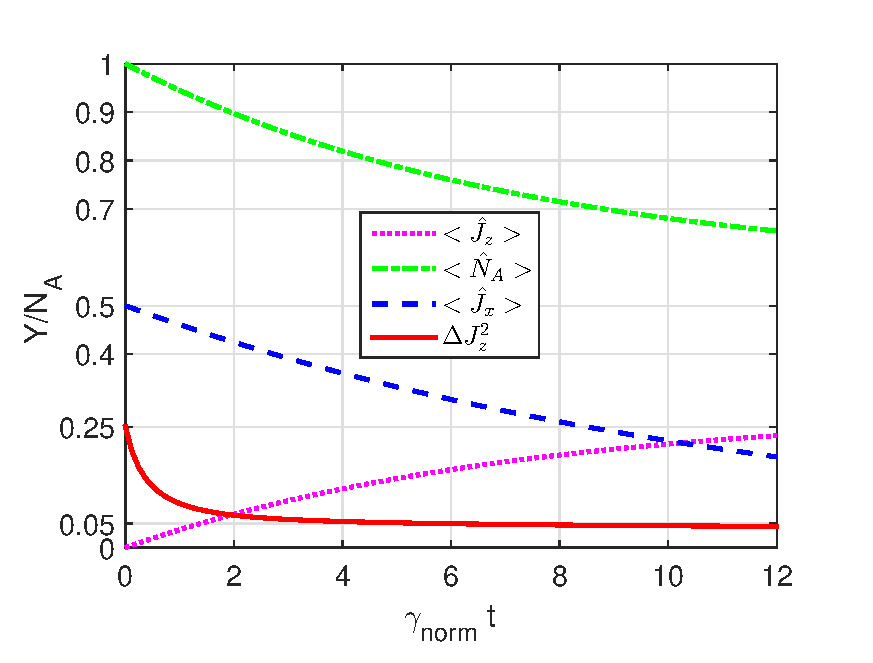
\includegraphics[scale=0.45]{../media/Figs/clockdynamics_m33_yq_rp1d5_exact}}
\end{minipage}
\begin{minipage}{.5\linewidth}
\centering
\subfloat[]{\label{fig:clockdynamics_m33_yq_rp1d5_approx}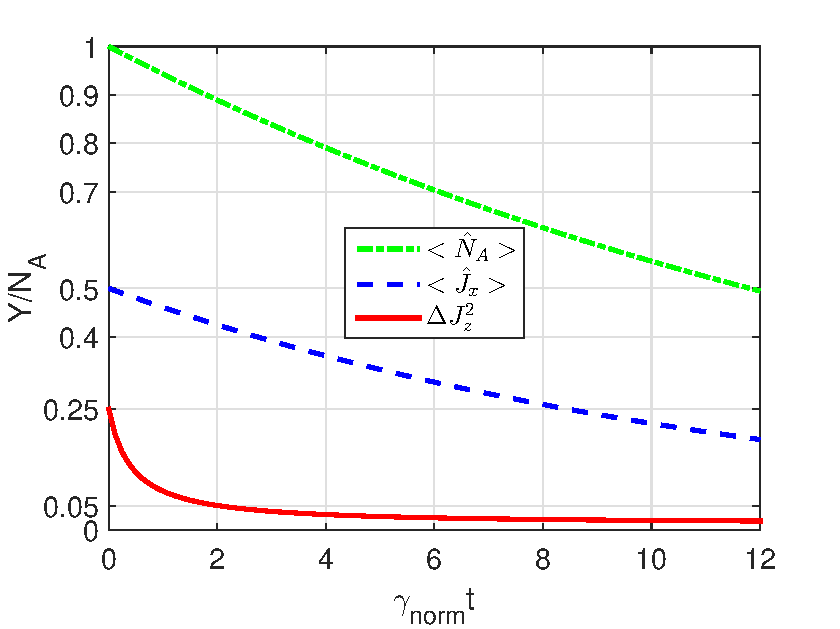
\includegraphics[scale=0.45]{../media/Figs/clockdynamics_m33_yq_rp1d5_approx}}
\end{minipage}
\par\medskip
\begin{minipage}{.5\linewidth}
\centering
\subfloat[]{\label{fig:clockdynamics_m44_yq_rp1d5_exact}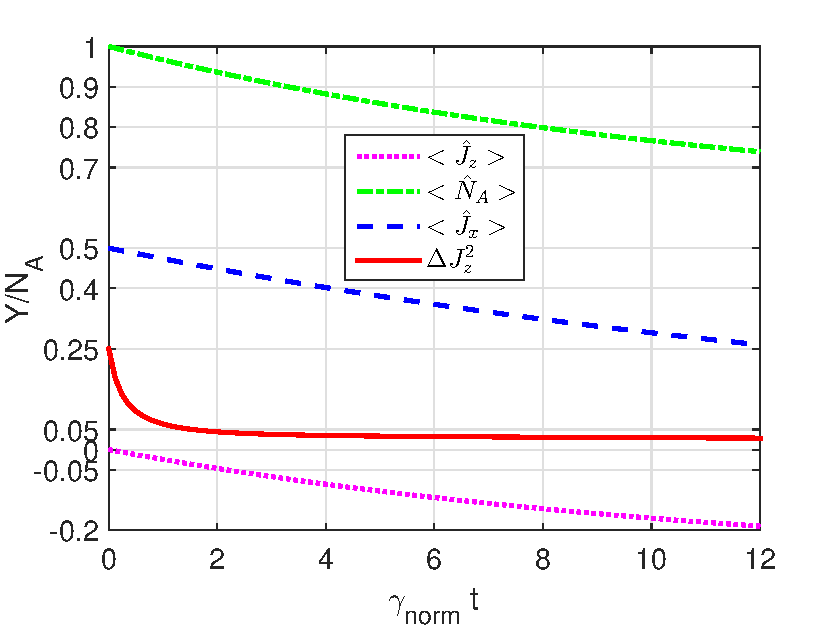
\includegraphics[scale=0.45]{../media/Figs/clockdynamics_m44_yq_rp1d5_exact}}
\end{minipage}
\begin{minipage}{.5\linewidth}
\centering
\subfloat[]{\label{fig:clockdynamics_m44_yq_rp1d5_approx}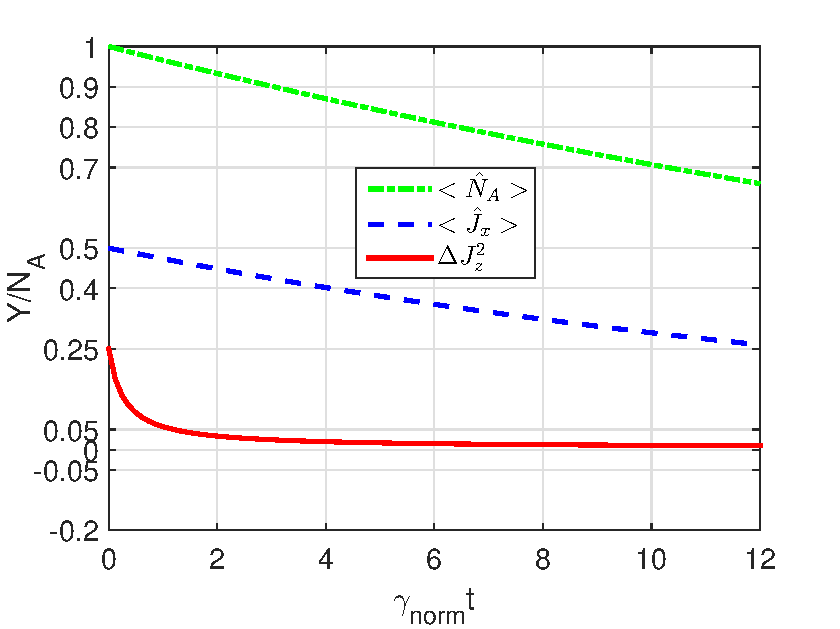
\includegraphics[scale=0.45]{../media/Figs/clockdynamics_m44_yq_rp1d5_approx}}
\end{minipage}
\caption{Evolution of expectation values of collective spin operators as a function of time with $ N_A=1000 $ atoms trapped at $ r'\!_\perp =1.5a $ along the $ H/x $-axis of the nanofiber. Subfigs.~\protect\subref{fig:clockdynamics_m33_yq_rp1d5_exact} and~\protect\subref{fig:clockdynamics_m33_yq_rp1d5_approx} use the magic frequencies close to the $ F=3\leftrightarrow F'=3 $ transition frequency $ \omega_{33'} $. Subfigs.~\protect\subref{fig:clockdynamics_m44_yq_rp1d5_exact} and~\protect\subref{fig:clockdynamics_m44_yq_rp1d5_approx} used the magic frequencies close to $ \omega_{44'} $. The $ \phi $-axis was defined as the quantization axis for these plots. Subfigs.~\protect\subref{fig:clockdynamics_m33_yq_rp1d5_exact} and~\protect\subref{fig:clockdynamics_m44_yq_rp1d5_exact} were calculated using the exact solution of the coupled differential equations of the expectation values of spin operators. In contrast, Subfigs.~\protect\subref{fig:clockdynamics_m33_yq_rp1d5_approx} and~\protect\subref{fig:clockdynamics_m44_yq_rp1d5_approx} use approximations by ignoring the dynamics of $ \expect{\hat{J}_z} $ for all calculations, and treat $ \expect{\hat{N}_A} $ as a constant in solving the differential equation for $ \Delta J_z^2 $. Other parameters used: $ \Omega/2\pi=52 $ MHz (does not matter). }\label{fig:clockdynamics_m_yq_rp1d5}
\end{figure}

\begin{figure}
\begin{minipage}{.5\linewidth}
\centering
\subfloat[]{\label{fig:xi_magic33_yq}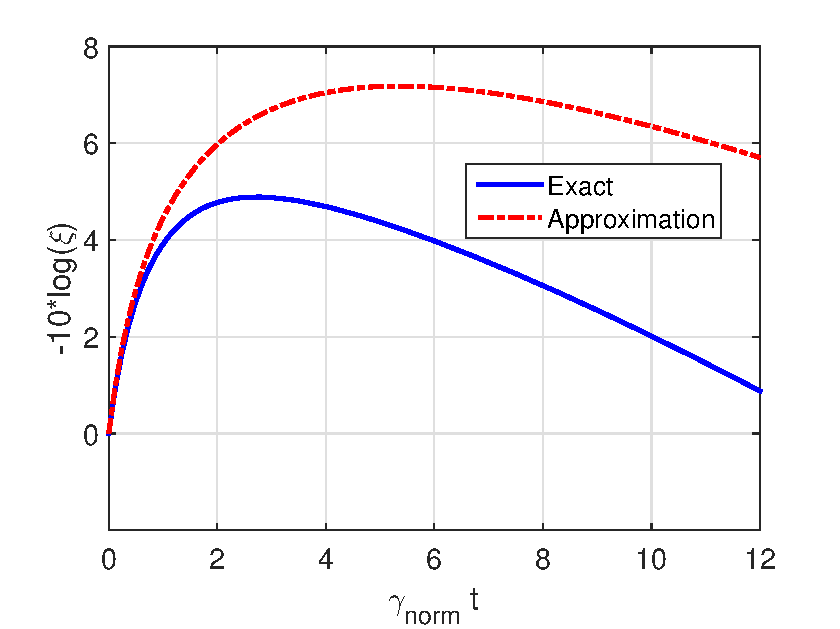
\includegraphics[scale=0.45]{../media/Figs/xi_magic33_yq}}
\end{minipage}
\begin{minipage}{.5\linewidth}
\centering
\subfloat[]{\label{fig:xi_magic44_yq}\includegraphics[scale=0.45]{../media/Figs/xi_magic44_yq}}
\end{minipage}
\par\medskip
\begin{minipage}{.5\linewidth}
\centering
\subfloat[]{\label{fig:xi_magic33_xq}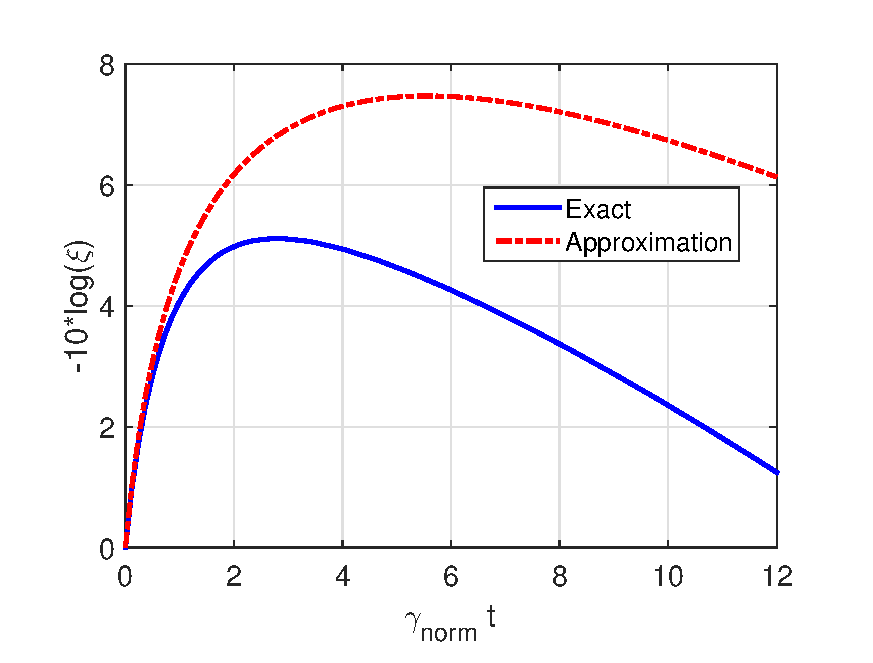
\includegraphics[scale=0.45]{../media/Figs/xi_magic33_xq}}
\end{minipage}
\begin{minipage}{.5\linewidth}
\centering
\subfloat[]{\label{fig:xi_magic44_xq}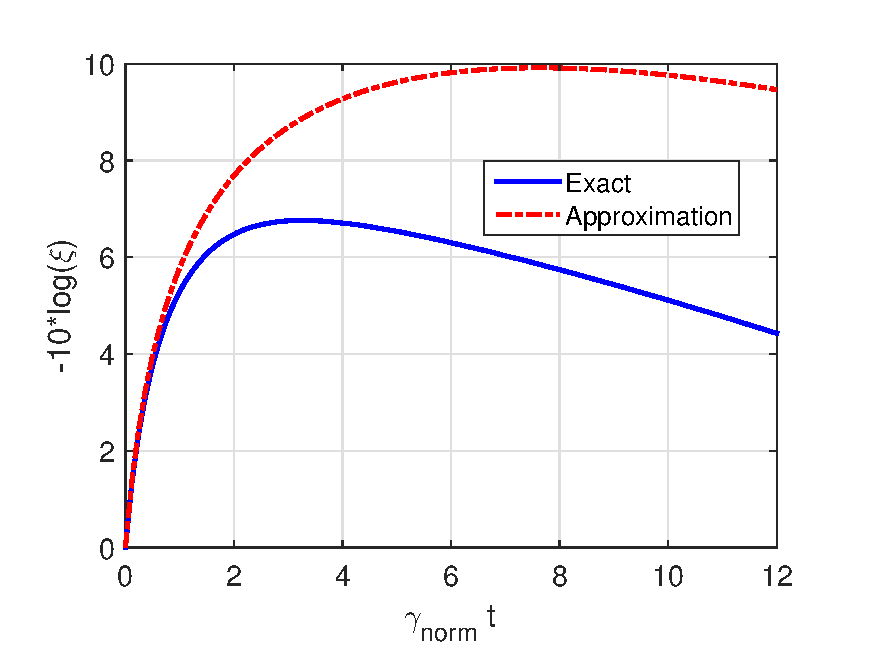
\includegraphics[scale=0.45]{../media/Figs/xi_magic44_xq}}
\end{minipage}
%\centering\makebox[\textwidth]{
%\includegraphics[width=0.65\textwidth]{./Figs/xi_magic44_yq}}
\caption{Spin squeezing evolution as a function of time with $ N_A=1000 $ atoms trapped at $ r'\!_\perp =1.5a $ along the $ H/x $-axis of the nanofiber. Subfigs.~\protect\subref{fig:xi_magic33_yq} and~\protect\subref{fig:xi_magic33_xq} use the magic frequencies close to the $ F=3\leftrightarrow F'=3 $ transition frequency $ \omega_{33'} $. Subfigs.~\protect\subref{fig:xi_magic44_yq} and~\protect\subref{fig:xi_magic44_xq} used the magic frequencies close to $ \omega_{44'} $. The magic frequencies and spin squeezing parameters are different for different choices of quantization axis. Subfigs.~\protect\subref{fig:xi_magic33_yq} and~\protect\subref{fig:xi_magic44_yq} define $ \phi $-axis as the quantization axis. In contrast, subfigs.~\protect\subref{fig:xi_magic33_xq} and~\protect\subref{fig:xi_magic44_xq} use $ r\!_\perp $-axis as the quantization axis. When $ z $-axis is chosen to be the quantization axis, almost no squeezing effect can be observed at the magic frequencies. As can be seen, when the quantization axis close to the local field direction, the spin squeezing parameter can reach to a higher value. Other parameters used: $ \Omega/2\pi=52 $ MHz (does not matter). }\label{fig:xi_magic}
\end{figure}



\newpage

\subsubsection{The microscopic perspective analysis of continuous measurement and spin squeezing}

The measurement operator after the probe light interacting with the ensemble of atoms can be given by
\begin{align}
\hat{\mathcal{M}} &= \sum_i^{N_A} \int_0^T \mathrm{d}t' \hat{X}_{\bar{D}}^{\rm out} (z_D,t'-(z_{D}-z_i')/v_p),\label{eq:Mxout}
\end{align}
where $ T $ and $ Z_D $ are the integration time and position of the detector, $ z_i' $ is the $ z $-coordinate of the $ i $-th atom. 
 

For each atom, using the effective Hamiltonian that causes the birefringence effect, 
\begin{align}
\hat{H}_{\rm eff} &= \hbar \chi_{\rm eff} \sqrt{\frac{\dot{N}_L}{2}} \hat{F}_z \hat{P}_{\bar{D}}
\end{align}
one can find the equation of motion for the quadrature operator $ \hat{X}_{\bar{D}} $ to be
\begin{align}
\dt{\hat{X}_{\bar{D}}(z,t)} &= -\frac{i}{\hbar} \left[ \hat{H}_{\rm eff},\hat{X}_{\bar{D}} \right] \\
\Leftrightarrow \pp{\hat{X}_{\bar{D}}(z,t)}{t}+v_g\pp{\hat{X}_{\bar{D}}(z,t)}{z} &=  \chi_{\rm eff} \sqrt{\frac{\dot{N}_L}{2}} \hat{F}_z.
\end{align}
A formal solution can be given by
\begin{align}
\hat{X}_{\bar{D}} (z,t) &= \hat{X}_{\bar{D}}(0,t-z/v_p) + \sqrt{\frac{\kappa}{2}}\hat{F}_z(t-(z-z'_i)/v_p)\Theta(z-z'_i),
\end{align} 
where the measurement strength per atom is defined as $ \kappa = \chi_{\rm eff}^2 \dot{N}_L $. 

Using the result above, Equ.~\ref{eq:Mxout} gives
\begin{align}
\hat{\mathcal{M}}(T) &= N_A\int_0^T\mathrm{d}t \hat{X}_{\bar{D}}(0,t-z_D/v_p) + N_A \sqrt{\frac{\kappa}{2}}\int_0^T\mathrm{d}t\hat{F}_z(t)\\
&\approx N_A\int_0^T\mathrm{d}t \hat{X}_{\bar{D}}(0,t-z_D/v_p) + N_AT\sqrt{\frac{\kappa}{2}}\hat{F}_z.
\end{align}
In the last step, we have used the fact that all atoms around a nanofiber are interacting with the probe light in the same manner, and we have assumed the transition time of the light passing through the ensemble of atoms is much shorter than the atomic dynamics and the sampling time of the detector. 

Since the setup of the photon detectors imply a vacuum state of the photonic operators. The mean value of the measurement can be given by 
\begin{align}
\expect{\hat{\mathcal{M}}}(T) &\approx N_AT\sqrt{\frac{\kappa}{2}}\expect{\hat{F}_z(0)}.
\end{align}

The variance of the measurement can be described by
\begin{align}
\Delta \mathcal{M}^2(T) &= \expect{\hat{\mathcal{M}}^2}-\expect{\hat{\mathcal{M}}}^2\\
&= N_A^2 \int_0^T\mathrm{d}t \int_0^T\mathrm{d}t'  \expect{\Delta\hat{X}_{\bar{D}}(0,t-z_D/v_p)\Delta\hat{X}_{\bar{D}}(0,t'-z_D/v_p)} \nonumber\\
&\quad + N_A^2 \frac{\kappa}{2} \int_0^T\mathrm{d}t \int_0^T\mathrm{d}t'\expect{\Delta\hat{F}_z(t)\Delta\hat{F}_z(t')}\\
&\approx \frac{N_A^2T}{2} + \frac{\kappa N_A^2T^2}{2} \Delta\hat{F}_z^2\\
&\equiv \Delta \mathcal{M}_{\rm SN}^2 + \Delta\mathcal{M}_{\rm PN}^2.
\end{align}
To derive the result above, we have used the fact that the covariance $ \expect{\Delta\hat{X}_{\bar{D}}(0,t-z_D/v_p)\Delta\hat{X}_{\bar{D}}(0,t'-z_D/v_p)}\equiv \expect{\hat{X}_{\bar{D}}(0,t-z_D/v_p)\hat{X}_{\bar{D}}(0,t'-z_D/v_p)}-\expect{\hat{X}_{\bar{D}}(0,t-z_D/v_p)}\expect{\hat{X}_{\bar{D}}(0,t'-z_D/v_p)}=\delta(t-t')/2 $ for the vacuum fluctuations, which leads to the vacuum shot noise $ \Delta \mathcal{M}_{\rm SN}^2=\frac{N_A^2T}{2} $. The additional projection noise, $ \Delta\mathcal{M}_{\rm PN}^2=\frac{\kappa N_A^2T^2}{2} \Delta\hat{F}_z^2(0) $, is the signal comes from the variance of the $ z $-projection of the collective spin state.  

...

Using the results above, one can write the stochastic master equation for the continuous measurement with the probe light discussed in this section...


\subsection{Sensitivity of the birefringence measurement using the clock states}
\textcolor{red}{To answer the question in this section: How to relate this to the critical shot noise limit--Equ.~\eqref{eq:shotnoise}?}  

For the birefringence measurement of the clock states discussed above, the fluctuation of the $ S_3 $ measurement is a combination effect of the shot noise fluctuation of the photon detector and the projection noise as the signal to determine the collective spin state:
\begin{align}
\Delta M^2 &= \Delta\mathcal{M}_{\rm SN}^2 + \Delta\mathcal{M}_{\rm PN}^2\\
&\equiv \Delta P^2_{SN} + \Delta P^2_S .
\end{align}
As have been discussed in Section~\ref{sec:birefringenceresolution}, the smallest detectable spin polarization is determined by the shot noise limit condition that 
\begin{align}
\Delta P_S = \Delta P_{SN},
\end{align}
where the standard variance of the signal can be estimated by
\begin{align}
\Delta P_S=P_0 \sin(\varphi_{_N}) \approx P_0 \varphi_{_N}
\end{align}
and the shot noise variance is determined by
\begin{align}
\Delta P_{SN} = \sqrt{\frac{P_0 \hbar \omega_0 }{2\eta \tau_{pd}}}.
\end{align}
We estimate the phase difference as
\begin{align}
\varphi_{_N} &= N_A \chi_{e\!f\!f}=N_A [(\chi_{H,\uparrow}-\chi_{H,\downarrow})-(\chi_{V,\uparrow}-\chi_{V,\downarrow})]\\
&= 2N_AC_{j'}^{(0)}(\Gamma_{H}^{1D}-\Gamma_V^{1D})\frac{1}{\Delta}=\frac{C_{j'}^{(0)}\sigma_0\Gamma_{vac}}{2}(\frac{1}{A^H_{e\!f\!f}}-\frac{1}{A^V_{e\!f\!f}})\frac{1}{\Delta}\\
&=N_AC_{j'}^{(0)}n_g\sigma_0\frac{\Gamma_{vac}}{2\Delta}\left[| \mathbf{u}_H(r'_{\!\perp})|^2- | \mathbf{u}_V(r'_{\!\perp})|^2 \right],
\end{align}
where $\frac{1}{\Delta}=\frac{1}{2}\sum_{f'}(\frac{1}{\Delta_{f',4}}-\frac{1}{\Delta_{f',3}})\approx \frac{1}{\Delta_{f',4}}$.

Now, we consider the critical case: $\eta =100\%$ and $\tau_{pd} = \frac{1}{\gamma_s}$, where the photon scattering rate
\begin{align*}
\gamma_s &= \sigma(\Delta) \frac{I(\br')}{\hbar \omega_0} \\
\sigma(\Delta) &=\frac{\sigma_0}{1+\frac{4\Delta^2}{\Gamma^2_{vac}}}\approx \sigma_0 \frac{\Gamma_{vac}^2}{4\Delta^2} \quad \text{(far detuning.)}
\end{align*}
We can rewrite 
\begin{align}
\Delta P_{SN} &=P_0\sqrt{\frac{ \sigma_0 }{2A_{in}}}\frac{\Gamma_{vac}}{2\Delta},\\
\Delta P_S &= N_A C_{j'}^{(0)}P_0 \frac{\sigma_0}{A_{e\!f\!f}}\frac{\Gamma_{vac}}{2\Delta}, 
\end{align}
with the effective mode areas
\begin{align}
A_{in } &= \frac{P_0}{I(\br')}=\frac{2}{| \mathbf{u}_H(r'_{\!\perp})|^2+ | \mathbf{u}_V(r'_{\!\perp})|^2},\\
A_{e\!f\!f} &= \frac{1}{n_g\left[ | \mathbf{u}_H(r'_{\!\perp})|^2- | \mathbf{u}_V(r'_{\!\perp})|^2\right]}.
\end{align}
Therefore, the $ \Delta P_S = \Delta P_{SN}$ condition gives the resolution of the birefringence measurement in terms of the minimum atom number as
\begin{align}
N^{min}_A &= \frac{1}{C_{j'}^{(0)}}\sqrt{\frac{A_{e\!f\!f}^2}{A_{in}\sigma_0}}.
\end{align}

%</quantumdynamics>

\appendix

%<*basistransfHS>

\chapter{Spin-polarization coupling Hamiltonian and Stokes vectors under coordinate transformation}\label{chap:basistransfHS}
In this appendix, we will derive the equations of Stokes vector operators and spin-polarization interaction Hamiltonian due to polarization basis transformations.
A general basis transformation theory will be derived in the context of linear-polarization basis transformations, and will then be applied to the linear $ D/\bar{D} $- and circular $ R/L $-bases cases.

\section{Spin-polarization Hamiltonian and Stokes vector operators in a linear basis}
In general, we can define an arbitrary linear polarization basis by
\begin{align}
\left(\!\begin{array}{c}
\mathbf{e}_n \\ \mathbf{e}_{\bar{n}}
\end{array}\!\right) &= 
\left(\!\!\begin{array}{cc}
\cos\theta & \sin\theta \\
- \sin\theta & \cos\theta
\end{array}\!\!\right)\bullet
\left(\!\begin{array}{c}
\mathbf{e}_H \\ \mathbf{e}_V
\end{array}\!\right)
=\mathbf{R}(\theta)\bullet \left(\!\begin{array}{c}
\mathbf{e}_H \\ \mathbf{e}_V
\end{array}\!\right),
\end{align}
or the inversed relationship
\begin{align}
\left(\!\begin{array}{c}\mathbf{e}_H \\ \mathbf{e}_V\end{array}\!\right)&= \mathbf{R}^{-1}(\theta)\bullet\left(\!\begin{array}{c}\mathbf{e}_n \\ \mathbf{e}_{\bar{n}}\end{array}\!\right),
\end{align}
where $ \theta $ is the angle of the $ \mathbf{e}_n $ basis rotated from the $ H $-direction around $ z $-axis, and $ \mathbf{e}_{\bar{n}} $ is the basis vector $ 90^\circ $ from the $ \mathbf{e}_n $ direction; $ \mathbf{R}(\theta)=\mathbf{R}_z(\theta) $ is the Euler rotation matrix about the $ z $-axis by $ \theta $ in the real-number $ \mathbf{SO}(3) $ rotation group, which has the property that $ \mathbf{R}^{-1}(\theta)=\mathbf{R}^T(\theta)=\mathbf{R}(-\theta) $. 
More generally, the basis transformation matrix is an unitary matrix determined by two parameters (two degrees of freedom)--$ \theta $ and $ \phi $--corresponding to the rotating angles around one axis and an relative phase between the base components, which is in the $ \mathbf{SU}(2) $ group.
%We denote the general case with $ \mathbf{R}=\mathbf{R}(\theta,\phi) $, or in the form of two-step rotations around $ i $-axis and then around $ j $-axis by $ \mathbf{R}=\mathbf{R}_j(\theta)\mathbf{R}_i(\phi) $, always satisfying $ \mathbf{R}^{-1}=\mathbf{R}^\dagger $ for either rotations.

Not to be confused, we have also defined an operator space spanned by operator vectors, like $ \left(\!\begin{array}{cc}\mathbf{e}_n,&\mathbf{e}_{\bar{n}}\end{array}\! \right) $, which has vectors, tensors or operators as the elements.
We have also defined the bullet operator ($ \bullet $) in the operator vector space isomorphically the same as the dot ($ \cdot $) product or matrix product in the conventional vector space while the sign of $ \cdot $ can usually be ignored and we will denote complex conjugates explicitly if needed. 
$ \mathbf{R}(\theta) $ and its transformations is a tensor defined in the operator vector space as well.
When a conventional vector or tensor multiplies with an operator vector or tensor, we will use $ \cdot $ between them and the conventional vector or tensor will be formally treated as a scalar to be $ \cdot $ multiplied with the elements of the operator vector or tensor. 
Two operator vectors in a $ \bullet $ multiplication form a mutual covariant relationship in the operator space.
 
With the coordinate basis rotated passively, both the mode components and the field annihilation operators should be rotated actively by $ -\theta $ to be transformation-equivalent.
Written in the matrix form in the operator space, 
\begin{align}
\left(\!\begin{array}{c}\mathbf{u}_n \\ \mathbf{u}_{\bar{n}}\end{array}\!\right) &= \mathbf{R}^{-1}(\theta)\bullet\left(\!\begin{array}{c}\mathbf{u}_H \\ \mathbf{u}_V\end{array}\!\right)\\
\hat{\mathbf{a}}_{n,\bar{n}} &=\mathbf{R}^{-1}(\theta)\bullet \hat{\mathbf{a}}_{H,V},
\end{align}
where $ \hat{\mathbf{a}}_{n,\bar{n}}=[\hat{a}_n;\hat{a}_{\bar{n}}] $ and $ \hat{\mathbf{a}}_{H,V}=[\hat{a}_H;\hat{a}_V] $ are the annihilation operator vectors using the $ \{n,\bar{n} \} $ and $ \{H,V \} $ bases, respectively.
In our notation, we use $ [\cdot ;\cdots] $ notation to indicate $ 1\times n $ vectors as general matrices.

Using the definition in the $ \{ H,V\} $-basis of the Stokes operators (Eq.\eqref{eq:SaHVaRL}) and the annihilation operator basis transformation relationships above, one can rewrite the Stokes operators in the $ \{\mathbf{e}_n, \mathbf{e}_{\bar{n}}\} $ basis by
\begin{subequations}\label{eq:Snnbar}
\begin{align}
\hat{S}_0 &= \frac{1}{2}\left[\left(\!\begin{array}{cc}\hat{a}_n^\dagger,& \hat{a}_{\bar{n}}^\dagger\end{array} \!\right)\bullet\mathbf{R}_{[1,:]}^\dagger(\theta)\bullet\mathbf{R}_{[1,:]}(\theta)\bullet
\left(\!\begin{array}{c}\hat{a}_n\\ \hat{a}_{\bar{n}}\end{array} \!\right)
+ \left(\!\begin{array}{cc}\hat{a}_n^\dagger,& \hat{a}_{\bar{n}}^\dagger\end{array} \!\right)\bullet\mathbf{R}^\dagger_{[2,:]}(\theta)\bullet\mathbf{R}_{[2,:]}(\theta)\bullet
\left(\!\begin{array}{c}\hat{a}_n\\ \hat{a}_{\bar{n}}\end{array} \!\right) \right]\nn\\
&= \frac{1}{2}\left\{\left(\!\begin{array}{cc}\hat{a}_n^\dagger,& \hat{a}_{\bar{n}}^\dagger\end{array} \!\right)\bullet
\left[\left(\!\begin{array}{cc}\cos^2\theta,& \frac{1}{2}\sin 2\theta \\ \frac{1}{2}\sin 2\theta, & \sin^2\theta\end{array} \!\right)
+ \left(\!\begin{array}{cc}\sin^2\theta,& -\frac{1}{2}\sin 2\theta \\ -\frac{1}{2}\sin 2\theta, & \cos^2\theta\end{array} \!\right)\right]\bullet
\left(\!\begin{array}{c}\hat{a}_n\\ \hat{a}_{\bar{n}}\end{array} \!\right)\right\}\nn\\
&=\frac{1}{2} \left[\hat{a}_n^\dagger\hat{a}_n+\hat{a}_{\bar{n}}^\dagger\hat{a}_{\bar{n}} \right]\\
\hat{S}_1 &= \frac{1}{2}\left\{\left(\!\begin{array}{cc}\hat{a}_n^\dagger,& \hat{a}_{\bar{n}}^\dagger\end{array} \!\right)
\bullet\left[\mathbf{R}_{[1,:]}^\dagger(\theta)\bullet\mathbf{R}_{[1,:]}(\theta) - \mathbf{R}_{[2,:]}^\dagger(\theta)\bullet\mathbf{R}_{[2,:]}(\theta) \right]
\bullet\left(\!\begin{array}{c}\hat{a}_n\\ \hat{a}_{\bar{n}}\end{array} \!\right) \right\}\nn\\
&= \frac{1}{2} \left[\cos 2\theta \hat{a}_n^\dagger\hat{a}_n + \sin 2\theta \hat{a}_n^\dagger\hat{a}_{\bar{n}} + \sin 2\theta \hat{a}_{\bar{n}}^\dagger\hat{a}_n -\cos 2\theta \hat{a}_{\bar{n}}^\dagger\hat{a}_{\bar{n}} \right]\\
\hat{S}_2 &= \frac{1}{2}\left\{\left(\!\begin{array}{cc}\hat{a}_n^\dagger,& \hat{a}_{\bar{n}}^\dagger\end{array} \!\right)
\bullet\left[\mathbf{R}_{[1,:]}^\dagger(\theta)\bullet\mathbf{R}_{[2,:]}(\theta) + \mathbf{R}_{[2,:]}^\dagger(\theta)\bullet\mathbf{R}_{[1,:]}(\theta) \right]
\bullet\left(\!\begin{array}{c}\hat{a}_n\\ \hat{a}_{\bar{n}}\end{array} \!\right) \right\}\nn\\
&= \frac{1}{2} \left[-\sin 2\theta \hat{a}_n^\dagger\hat{a}_n + \cos 2\theta \hat{a}_n^\dagger\hat{a}_{\bar{n}} + \cos 2\theta \hat{a}_{\bar{n}}^\dagger\hat{a}_n +\sin 2\theta \hat{a}_{\bar{n}}^\dagger\hat{a}_{\bar{n}} \right]\\
\hat{S}_3 &= \frac{1}{2i}\left\{\left(\!\begin{array}{cc}\hat{a}_n^\dagger,& \hat{a}_{\bar{n}}^\dagger\end{array} \!\right)
\bullet\left[\mathbf{R}_{[1,:]}^\dagger(\theta)\bullet\mathbf{R}_{[2,:]}(\theta) - \mathbf{R}_{[2,:]}^\dagger(\theta)\bullet\mathbf{R}_{[1,:]}(\theta) \right]
\bullet\left(\!\begin{array}{c}\hat{a}_n\\ \hat{a}_{\bar{n}}\end{array} \!\right) \right\}\nn\\
&= \frac{1}{2i} \left[\hat{a}_n^\dagger\hat{a}_{\bar{n}} - \hat{a}_{\bar{n}}^\dagger\hat{a}_n  \right].
\end{align}
\end{subequations}
In deriving the equations above, we have denoted $ \mathbf{R}_{[i,:]}(\theta) $ as the $ i $-th row of $ \mathbf{R}(\theta) $ and $ \mathbf{R}_{[i,:]}^\dagger(\theta) $ as the conjugate transpose of the $ i $-th row of $ \mathbf{R}(\theta) $.
As a shorthand, these relationships of Stokes operators can be expressed as an operator transformation, $ \hat{\mathbf{S}}=\mathbf{M}\bullet\hat{\mathbf{A}}_{n,\bar{n}} $, where $ \hat{\mathbf{S}}=[\hat{S}_0;\hat{S}_1;\hat{S}_2;\hat{S}_3] $ and $ \hat{\mathbf{A}}_{n,\bar{n}}=[\hat{a}_n^\dagger\hat{a}_n;\hat{a}_n^\dagger\hat{a}_{\bar{n}};\hat{a}_{\bar{n}}^\dagger\hat{a}_n;\hat{a}_{\bar{n}}^\dagger\hat{a}_{\bar{n}}] $ are the operator vectors and $ \mathbf{M} $ is the transformation matrix defined by the transformation coefficients in Eqs.\eqref{eq:Snnbar}.
One can prove that the inversed transformation matrix $ \mathbf{M}^{-1}=2\mathbf{M}^\dagger $, and $ \mathbf{M} $ can be derived in the following form, in general,
\begin{align}
\mathbf{M} &=\frac{1}{2}\left(\!\begin{array}{c}
\mathrm{vec}_r\left[\mathbf{R}_{[1,:]}^\dagger(\theta)\mathbf{R}_{[1,:]}(\theta) + \mathbf{R}_{[2,:]}^\dagger(\theta)\mathbf{R}_{[2,:]}(\theta) \right]\\
\mathrm{vec}_r\left[\mathbf{R}_{[1,:]}^\dagger(\theta)\mathbf{R}_{[1,:]}(\theta) - \mathbf{R}_{[2,:]}^\dagger(\theta)\mathbf{R}_{[2,:]}(\theta) \right]\\
\mathrm{vec}_r\left[\mathbf{R}_{[1,:]}^\dagger(\theta)\mathbf{R}_{[2,:]}(\theta) + \mathbf{R}_{[2,:]}^\dagger(\theta)\mathbf{R}_{[1,:]}(\theta) \right]\\
-i\mathrm{vec}_r\left[\mathbf{R}_{[1,:]}^\dagger(\theta)\mathbf{R}_{[2,:]}(\theta) - \mathbf{R}_{[2,:]}^\dagger(\theta)\mathbf{R}_{[1,:]}(\theta) \right]
 \end{array} \!\right)\\
&= \frac{1}{2}\left(\!\begin{array}{cccc} 1,&0,&0,& 1\\
\cos 2\theta,&\sin 2\theta, & \sin 2\theta, & -\cos 2\theta\\
-\sin 2\theta, & \cos 2\theta, & \cos 2\theta, & \sin 2\theta\\
0,&-i,& i,& 0\end{array}\!\right),
\end{align}
where $ \mathrm{vec}_r[\cdot] $ means the vectorization of a matrix by concatenating its rows. 


By using the vector space representation, the E-field operator can be written in the $ \{n,\bar{n}\} $ basis by 
\begin{align}
\hat{\mathbf{E}}^{(+)}(\br;t) &= \sqrt{ \frac{2 \pi \hbar \omega_0}{ v_g} } \left[\mathbf{u}_H(r\!_\perp,\phi) \hat{a}_H(z,t) + \mathbf{u}_V(r\!_\perp,\phi) \hat{a}_V(z,t)\right]  e^{i (\beta_0 z- \omega_0 t)}\\
&= \sqrt{ \frac{2 \pi \hbar \omega_0}{ v_g} } \left(\!\begin{array}{cc}\mathbf{u}_H, & \mathbf{u}_V\end{array}\!\right)
\bullet \left(\!\begin{array}{c}\hat{a}_H\\ \hat{a}_V\end{array} \!\right)  e^{i (\beta_0 z- \omega_0 t)}\\
&= \sqrt{ \frac{2 \pi \hbar \omega_0}{ v_g} } \left(\!\begin{array}{cc}\mathbf{u}_H, & \mathbf{u}_V\end{array}\!\right)\bullet\mathbf{R}(\theta)
\bullet \mathbf{R}^{-1}(\theta)\bullet\left(\!\begin{array}{c}\hat{a}_H\\ \hat{a}_V\end{array} \!\right)  e^{i (\beta_0 z- \omega_0 t)}\\
&= \sqrt{ \frac{2 \pi \hbar \omega_0}{ v_g} } \left(\!\begin{array}{cc}\mathbf{u}_n, & \mathbf{u}_{\bar{n}}\end{array}\!\right)
\bullet \left(\!\begin{array}{c}\hat{a}_n\\ \hat{a}_{\bar{n}}\end{array} \!\right)  e^{i (\beta_0 z- \omega_0 t)}\\
&= \sqrt{ \frac{2 \pi \hbar \omega_0}{ v_g} } \left[\mathbf{u}_n(r\!_\perp,\phi) \hat{a}_n(z,t) + \mathbf{u}_{\bar{n}}(r\!_\perp,\phi) \hat{a}_{\bar{n}}(z,t)\right]  e^{i (\beta_0 z- \omega_0 t)}.\label{eq:Efieldop_nnbar}
\end{align}
As expected, the field operator preserves the form in the new basis as defined in Eq.\eqref{eq:Ebp}.

Therefore, the effective atom-light interaction Hamiltonian can be written as
\begin{align}
\hat{h}_\eff &= -\hat{\mathbf{E}}^{(-)}(\br')\cdot\hat{\tensor{\mathbf{\alpha}}}\cdot\hat{\mathbf{E}}^{(+)}(\br')\nn\\
&=-\frac{2 \pi \hbar \omega_0}{ v_g}
\left(\!\begin{array}{cc}\hat{a}_n^\dagger, & \hat{a}_{\bar{n}}^\dagger\end{array} \!\right)\bullet \left(\!\begin{array}{c}\mathbf{u}_n^*\\ \mathbf{u}_{\bar{n}}^*\end{array}\!\right)
\cdot\hat{\tensor{\mathbf{\alpha}}}\cdot
\left(\!\begin{array}{cc}\mathbf{u}_n, & \mathbf{u}_{\bar{n}}\end{array}\!\right)
\bullet \left(\!\begin{array}{c}\hat{a}_n\\ \hat{a}_{\bar{n}}\end{array} \!\right) \nn\\
&= \hbar \left(\!\begin{array}{cc}\hat{a}_n^\dagger, & \hat{a}_{\bar{n}}^\dagger\end{array} \!\right)\bullet
\left(\!\begin{array}{cc} \hat{\chi}_{nn},&\hat{\chi}_{n\bar{n}}\\
\hat{\chi}_{\bar{n}n},&\hat{\chi}_{\bar{n}\bar{n}}\end{array} \!\right)
\bullet\left(\!\begin{array}{c}\hat{a}_n\\ \hat{a}_{\bar{n}}\end{array} \!\right) \nn\\
&= \hbar \hat{\boldsymbol{\chi}}_{n,\bar{n}}^\dagger\bullet \hat{\mathbf{A}}_{n,\bar{n}}= \hbar \hat{\boldsymbol{\chi}}_{n,\bar{n}}^\dagger\bullet 2\mathbf{M}^\dagger\bullet \hat{\mathbf{S}}\\
&= \hbar\left\{(\hat{\chi}_{nn}+ \hat{\chi}_{\bar{n}\bar{n}})\hat{S}_0 \right.\nn\\
&\quad+ [\cos 2\theta \hat{\chi}_{nn}+ \sin 2\theta(\hat{\chi}_{n\bar{n}}+\hat{\chi}_{\bar{n}n}) - \cos 2\theta\hat{\chi}_{\bar{n}\bar{n}}]\hat{S}_1 \nn\\
&\quad+ [-\sin 2\theta \hat{\chi}_{nn}+ \cos 2\theta(\hat{\chi}_{n\bar{n}}+\hat{\chi}_{\bar{n}n}) + \sin 2\theta \hat{\chi}_{\bar{n}\bar{n}}]\hat{S}_2 \nn\\
&\quad+\left. i \left(\hat{\chi}_{n\bar{n}}-\hat{\chi}_{\bar{n}n}\right)\hat{S}_3 \right\}.\label{eq:heff_nnbarChiS}
\end{align}
In deriving the expression above, we have defined $\hat{\boldsymbol{\chi}}_{n,\bar{n}}=[\hat{\chi}_{nn};\hat{\chi}_{n\bar{n}};\hat{\chi}_{\bar{n}n};\hat{\chi}_{\bar{n}\bar{n}}]$ as the coupling operator vector.
The coupling coefficient elements of $ 2\mathbf{M}^\dagger $, $ 2M_{ij} $, correspond to the coupling coefficients in Eq.\eqref{eq:heff_nnbarChiS} between the spin operators in $ \hat{\boldsymbol{\chi}}_{n,\bar{n}} $ and the polarization operators in $ \hat{\mathbf{S}} $, and each column of $ 2\mathbf{M}^\dagger $ corresponds to the coefficients in the corresponding line of the $ \hat{S}_i $ coupling term in Eq.\eqref{eq:heff_nnbarChiS}.


If we set $ \theta=\pi/4 $, we will be in the $ \{\mathbf{e}_D,\mathbf{e}_{\bar{D}} \} $ basis.
\begin{subequations}
\begin{align}
\hat{a}_D &= \frac{1}{\sqrt{2}}(\hat{a}_H-\hat{a}_V)\\
\hat{a}_{\bar{D}} &= \frac{1}{\sqrt{2}}(\hat{a}_H+\hat{a}_V),
\end{align}
\end{subequations}
or,
\begin{subequations}
\begin{align}
\hat{a}_H &= \frac{1}{\sqrt{2}}(\hat{a}_D+\hat{a}_{\bar{D}})\\
\hat{a}_V &= \frac{1}{\sqrt{2}}(\hat{a}_{\bar{D}}-\hat{a}_D).
\end{align}
\end{subequations}
The Stokes operators becomes
\begin{subequations}
\begin{align}
\hat{S}_0 &= \frac{1}{2} \left[\hat{a}_D^\dagger\hat{a}_D+\hat{a}_{\bar{D}}^\dagger\hat{a}_{\bar{D}} \right]\\
\hat{S}_1 &= \frac{1}{2} \left[ \hat{a}_D^\dagger\hat{a}_{\bar{D}} +  \hat{a}_{\bar{D}}^\dagger\hat{a}_D \right]\\
\hat{S}_2 &= \frac{1}{2} \left[ \hat{a}_{\bar{D}}^\dagger\hat{a}_{\bar{D}}-\hat{a}_D^\dagger\hat{a}_D \right]\\
\hat{S}_3 &= \frac{1}{2i} \left[\hat{a}_D^\dagger\hat{a}_{\bar{D}}-\hat{a}_{\bar{D}}^\dagger\hat{a}_D \right].
\end{align}
\end{subequations}
The field operator becomes 
\begin{align}
\hat{\mathbf{E}}^{(+)}(\br;t) &=\sqrt{ \frac{2 \pi \hbar \omega_0}{ v_g} } \left[\mathbf{u}_D(r\!_\perp,\phi) \hat{a}_D(z,t)+\mathbf{u}_{\bar{D}}(r\!_\perp,\phi) \hat{a}_{\bar{D}}(z,t)  \right]e^{i (\beta_0 z- \omega_0 t)}.
\end{align}
The effective Hamiltonian can be simplified from Eq.\eqref{eq:heff_nnbarChiS} to 
\begin{align}
\hat{h}_\eff &= \hbar[(\hat{\chi}_{DD}+\hat{\chi}_{\bar{D}\bar{D}})\hat{S}_0 +(\hat{\chi}_{D\bar{D}}+\hat{\chi}_{\bar{D}D} )\hat{S}_1\nn\\
&\quad + (\hat{\chi}_{\bar{D}\bar{D}}-\hat{\chi}_{DD})\hat{S}_2 +i(\hat{\chi}_{D\bar{D}}-\hat{\chi}_{\bar{D}D} )\hat{S}_3].
\end{align}
The Hamiltonian expression above should satisfy the cyclical transformation from the $ H $- and $ V $-basis expression.

\section{Spin-polarization Hamiltonian and Stokes vector operators in a circular basis}
We define a set of polarization vector transformation relationships by 
\begin{subequations}
\begin{align}
\hat{a}_H &= \frac{1}{\sqrt{2}}(\hat{a}_R+\hat{a}_L )\\
\hat{a}_V &= \frac{i}{\sqrt{2}}(\hat{a}_R-\hat{a}_L ),
\end{align}
\end{subequations}
or the inverse
\begin{subequations}
\begin{align}
\hat{a}_R &= \frac{1}{\sqrt{2}}(\hat{a}_H-i\hat{a}_V )\\
\hat{a}_L &= \frac{1}{\sqrt{2}}(\hat{a}_H+i\hat{a}_V ),
\end{align}
\end{subequations}
where $ R $($ L $) indicates the right(left)-circularly polarized mode.
The Stokes operators can then be defined in both linear ($ H $ and $ V $) and circular ($ L $ and $ R $) polarization bases by
\begin{subequations}\label{eq:SaHVaRL}
\begin{align}
\hat{S}_0 &= \frac{1}{2} \left[\hat{a}_H^\dagger\hat{a}_H+\hat{a}_V^\dagger\hat{a}_V \right] = \frac{1}{2} \left[\hat{a}_R^\dagger\hat{a}_R+\hat{a}_L^\dagger\hat{a}_L \right]\\
\hat{S}_1 &= \frac{1}{2} \left[\hat{a}_H^\dagger\hat{a}_H-\hat{a}_V^\dagger\hat{a}_V \right] = \frac{1}{2} \left[\hat{a}_R^\dagger\hat{a}_L+\hat{a}_L^\dagger\hat{a}_R \right]\\
\hat{S}_2 &= \frac{1}{2} \left[\hat{a}_H^\dagger\hat{a}_V+\hat{a}_V^\dagger\hat{a}_H \right] = \frac{i}{2} \left[\hat{a}_L^\dagger\hat{a}_R-\hat{a}_R^\dagger\hat{a}_L \right]\\
\hat{S}_3 &= \frac{1}{2i} \left[\hat{a}_H^\dagger\hat{a}_V-\hat{a}_V^\dagger\hat{a}_H \right] = \frac{1}{2} \left[\hat{a}_R^\dagger\hat{a}_R-\hat{a}_L^\dagger\hat{a}_L \right].
\end{align}
\end{subequations}
The inversed transformations can be easily derived by inverting the transformation coefficient matrices. 

Based on Eq.\eqref{eq:Ebp}, when the input probe can be decomposed into degenerate orthonormal guided modes in the $H/V $ or $ R/L $ bases, the E-field operator can be written in the quasilinear and quasicircular mode bases by 
\begin{align}
\hat{\mathbf{E}}^{(+)}(r\!_\perp,\phi,z;t) &= \sqrt{ \frac{2 \pi \hbar \omega_0}{ v_g} } \left[\mathbf{u}_H(r\!_\perp,\phi) \hat{a}_H(z,t) + \mathbf{u}_V(r\!_\perp,\phi) \hat{a}_V(z,t)\right]  e^{i (\beta_0 z- \omega_0 t)}\\
&= \sqrt{ \frac{2 \pi \hbar \omega_0}{ v_g} } \left[\mathbf{u}_R(r\!_\perp,\phi) \hat{a}_R(z,t) + \mathbf{u}_L(r\!_\perp,\phi) \hat{a}_L(z,t)\right]  e^{i (\beta_0 z- \omega_0 t)}.
\end{align}
Therefore, the effective atom-light interaction Hamiltonian can be given in those bases by 
\begin{align}
\hat{h}_\eff &= -\hat{\mathbf{E}}^{(-)}(\br')\cdot\hat{\tensor{\mathbf{\alpha}}}\cdot\hat{\mathbf{E}}^{(+)}(\br')\nn\\
&= \hbar\left[(\hat{\chi}_{HH}+\hat{\chi}_{VV})\hat{S}_0 + (\hat{\chi}_{HH}-\hat{\chi}_{VV})\hat{S}_1 + (\hat{\chi}_{HV}+\hat{\chi}_{VH})\hat{S}_2 + i(\hat{\chi}_{HV}-\hat{\chi}_{VH})\hat{S}_3 \right]\\
&= \hbar\left[(\hat{\chi}_{RR}+\hat{\chi}_{LL})\hat{S}_0 + (\hat{\chi}_{RL}+\hat{\chi}_{LR})\hat{S}_1 + i(\hat{\chi}_{RL}-\hat{\chi}_{LR})\hat{S}_2 + (\hat{\chi}_{RR}-\hat{\chi}_{LL})\hat{S}_3 \right]\\
&=\hbar\sum_{i=0}^3 \hat{\chi}_{i}\hat{S}_i\\
&=\hbar\sum_{i,j=0} \chi_{ij}\hat{f}_i\hat{S}_j,
\end{align}
with $\hat{\chi}_{pp'} $ defined in Eq.\eqref{eq:chippp}.

%</basistransfHS>

%###################################################################################
\bibliographystyle{../styles/abbrv-alpha-letters-links}
\bibliography{../refs/Archive}
%%%%%%%%%%%%%%%%%%%%%%%%%%%%%%%%%%%%%%%%%%%%%%%%%%%%%%%%%%%%%%%%%%%%%%%%%%%%%%%%%%%%

\printindex
\end{document}